\documentclass[11pt,a4paper,twoside]{book}
\usepackage[T1]{fontenc}
\usepackage[utf8]{inputenc}
\usepackage{mathpazo}
\usepackage[scaled=0.90]{helvet}
\usepackage{courier}
\usepackage[a4paper,inner=3.0cm,outer=2.4cm,top=2.6cm,bottom=2.8cm]{geometry}
\usepackage{xcolor}
\usepackage{tikz}
\usetikzlibrary{calc}
\usepackage{booktabs}
\usepackage{array}
\usepackage{enumitem}
\usepackage[german=quotes]{csquotes}
\usepackage{fancyhdr}
\usepackage{titlesec}
\usepackage{amsmath,amssymb}
\usepackage{tcolorbox}
\tcbuselibrary{skins,breakable}
\usepackage[hidelinks]{hyperref}

\definecolor{tief}{HTML}{1F3A5F}
\definecolor{mittel}{HTML}{2E5F8A}
\definecolor{akzent}{HTML}{A34A28}
\definecolor{sand}{HTML}{F4F1EA}
\definecolor{grau}{HTML}{5A5A5A}
\definecolor{gruen}{HTML}{2F6B4F}
\definecolor{purpur}{HTML}{5B3A72}

\newcolumntype{P}[1]{>{\raggedright\arraybackslash}p{#1}}

\newcommand{\kursiv}[1]{{\itshape\color{grau}#1}}
\newcommand{\code}[1]{{\ttfamily\small #1}}
\newcommand{\Person}[1]{\textbf{#1}}
\newcommand{\Begriff}[1]{\textbf{#1}}
\newcommand{\zit}[1]{\textsuperscript{[#1]}}
\newcommand{\Oh}{\mathcal{O}}
\newcommand{\boxtitel}[1]{{\bfseries\color{tief}#1}\par\vspace{6pt}}
\newcommand{\boxtitelr}[1]{{\bfseries\color{akzent}#1}\par\vspace{6pt}}
\newcommand{\loesung}{\par\vspace{8pt}{\bfseries\color{mittel}Lösung}\par\vspace{4pt}}

\newtcolorbox{grundbox}[1][tief]{
  breakable, enhanced, colback=sand, colframe=sand,
  boxrule=0pt, leftrule=3pt, borderline west={3pt}{0pt}{#1},
  left=12pt, right=10pt, top=10pt, bottom=10pt,
  sharp corners, before skip=12pt, after skip=12pt}

\newenvironment{merksatz}{\begin{grundbox}[tief]}{\end{grundbox}}
\newenvironment{warnung}{\begin{grundbox}[akzent]}{\end{grundbox}}
\newenvironment{technik}{\begin{grundbox}[mittel]}{\end{grundbox}}
\newenvironment{aktuell}{\begin{grundbox}[gruen]}{\end{grundbox}}
\newenvironment{definition}{\begin{grundbox}[purpur]}{\end{grundbox}}
\newenvironment{aufgabe}{\begin{grundbox}[grau]\boxtitel{Übungsaufgaben}}{\end{grundbox}}
\newtcolorbox{geschichte}[1][]{
  breakable, enhanced, colback=sand, colframe=sand,
  boxrule=0pt, borderline west={3pt}{0pt}{purpur},
  left=12pt, right=10pt, top=10pt, bottom=10pt,
  sharp corners, before skip=12pt, after skip=12pt,
  title=\relax, #1}
\tcbset{gestitel/.style={}}

\titleformat{\chapter}[display]
  {\normalfont\huge\bfseries\color{tief}}{\Large\color{grau}Kapitel \thechapter}{8pt}{\Huge}
\titleformat{\part}[display]
  {\normalfont\huge\bfseries\color{tief}\filcenter}{\Large\color{grau}Teil \thepart}{10pt}{\Huge}
\titlespacing*{\chapter}{0pt}{10pt}{28pt}

\pagestyle{fancy}
\fancyhf{}
\fancyhead[LE,LO]{\small\itshape\color{grau}\leftmark}
\fancyfoot[LE,LO]{\small\color{grau}\thepage}
\renewcommand{\headrulewidth}{0.4pt}
\renewcommand{\footrulewidth}{0pt}
\renewcommand{\chaptermark}[1]{\markboth{#1}{}}
\hyphenation{be-grün-den Ent-wurfs-do-ku-men-te Sprich-wort-samm-lung
Aus-las-sung Aus-las-sun-gen Schnitt-stel-len Zu-sam-men-set-zung
Ne-ben-läu-fig-keit Feh-ler-be-hand-lung Über-tra-gungs-schicht
Spei-cher-be-rei-ni-gung Wie-der-ho-lung Vor-her-sag-bar-keit
Da-ten-mo-dell Ge-ne-ri-zi-tät Pro-gram-mie-rer Ver-er-bung}
\setlength{\parindent}{0pt}
\setlength{\parskip}{6pt}
\renewcommand{\arraystretch}{1.4}

\title{Vom Programm zum Werk}
\author{}
\date{}

\begin{document}
\frontmatter
\thispagestyle{empty}
\begin{center}
\vspace*{2.2cm}
{\color{grau}\scshape\large Informatik von Grund auf --- Band 23}\\[1.8cm]
{\color{tief}\fontsize{36}{42}\selectfont\bfseries Vom Programm\\[4pt] zum Werk}\\[1.0cm]
{\color{akzent}\Large Sprachübergreifende Entscheidungen}\\[1.6cm]
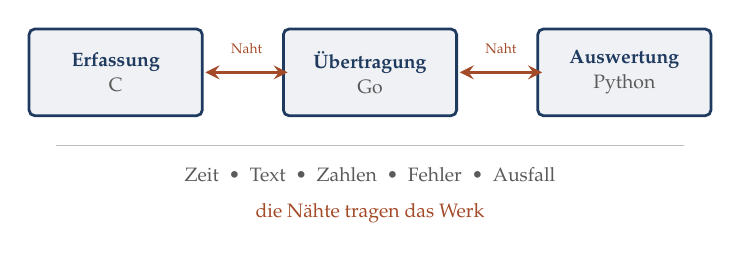
\begin{tikzpicture}[scale=0.95]
  \node[draw=tief, fill=tief!7, line width=1.0pt, rounded corners=2pt, inner sep=6pt, minimum width=2.20cm, minimum height=1.10cm, align=center, font=\scriptsize, text=tief] at (1.30,1.60) {\textbf{Erfassung}\\[1pt]{\color{grau}C}};
  \node[draw=tief, fill=tief!7, line width=1.0pt, rounded corners=2pt, inner sep=6pt, minimum width=2.20cm, minimum height=1.10cm, align=center, font=\scriptsize, text=tief] at (4.70,1.60) {\textbf{Übertragung}\\[1pt]{\color{grau}Go}};
  \node[draw=tief, fill=tief!7, line width=1.0pt, rounded corners=2pt, inner sep=6pt, minimum width=2.20cm, minimum height=1.10cm, align=center, font=\scriptsize, text=tief] at (8.10,1.60) {\textbf{Auswertung}\\[1pt]{\color{grau}Python}};
  \draw[akzent, line width=1.2pt, <->, >=stealth] (2.50,1.60)--(3.60,1.60);
  \draw[akzent, line width=1.2pt, <->, >=stealth] (5.90,1.60)--(7.00,1.60);
  \node[font=\tiny, color=akzent] at (3.05,1.92) {Naht};
  \node[font=\tiny, color=akzent] at (6.45,1.92) {Naht};
  \draw[grau!40, line width=0.5pt] (0.5,0.62)--(8.9,0.62);
  \node[font=\scriptsize, color=grau] at (4.70,0.24) {Zeit \ \textbullet\ \ Text \ \textbullet\ \ Zahlen \ \textbullet\ \ Fehler \ \textbullet\ \ Ausfall};
  \node[font=\scriptsize, color=akzent] at (4.70,-0.28) {die Nähte tragen das Werk};
\end{tikzpicture}\\[1.6cm]
{\color{grau}Was bleibt, wenn die Sprache wegfällt}\\[4pt]
{\color{grau}Jeder Schritt erklärt. Mit vollständig entwickelten Programmen.}\\[2.6cm]
{\color{grau}\small Stand der Forschung: August 2026}
\end{center}
\clearpage
\thispagestyle{empty}
\vspace*{\fill}
\begin{flushleft}
{\small\color{grau}
\textbf{\color{tief}Informatik von Grund auf} --- Band 23\\[2pt]
\textit{Vom Programm zum Werk} $\cdot$ Programme, die zusammenwirken\\[14pt]

Herausgeber und Urheber: Jürgen Maier\\[2pt]
Entstanden 2026 in Zusammenarbeit mit Claude (Anthropic); Konzeption, Vorgaben, Prüfung und Herausgeberschaft: Jürgen Maier.\\[14pt]

\textbf{Lizenz}\\[2pt]
Dieses Werk ist lizenziert unter einer Creative-Commons-Lizenz \textbf{Namensnennung -- Weitergabe unter gleichen Bedingungen 4.0 International (CC BY-SA 4.0)}. Sie dürfen das Werk vervielfältigen, verbreiten, bearbeiten und auch kommerziell nutzen, sofern Sie den Urheber nennen und Bearbeitungen unter derselben Lizenz weitergeben.\\[2pt]
Lizenztext: \texttt{https://creativecommons.org/licenses/by-sa/4.0/legalcode.de}\\[14pt]

\textbf{Quellen und Fassungen}\\[2pt]
Quelltexte, Fehlermeldungen und aktuelle Fassungen aller Bände:\\
\texttt{https://github.com/juergenmaier2026/informatik-von-grund-auf}\\[2pt]
Dauerhaft archiviert bei Zenodo: \texttt{https://doi.org/10.5281/zenodo.23773283}\\[2pt]
Schwesterreihe: \textit{Mathematik von Grund auf}, \texttt{https://doi.org/10.5281/zenodo.23698547}\\[14pt]

\textbf{Zitiervorschlag}\\[2pt]
Maier, J. (2026). \textit{Informatik von Grund auf, Band 23: Vom Programm zum Werk}. Fassung 1.0.1. \texttt{https://doi.org/10.5281/zenodo.23773283}\\[14pt]

Satz: \LaTeX{} mit Palatino. Fassung 1.0.1, Oktober 2026. 122 Seiten.
}
\end{flushleft}
\vspace*{1.5cm}
\clearpage

\cleardoublepage
\tableofcontents
\mainmatter
\chapter*{Vorwort: Die Nähte}
\addcontentsline{toc}{chapter}{Vorwort}
\markboth{Vorwort}{Vorwort}

\textbf{Drei Bände haben gezeigt, wie man in einer Sprache gut arbeitet.} \kursiv{Dieser handelt davon, was geschieht, wenn drei solche Teile zusammengefügt werden --- und warum die Fehler dann fast alle an den Nähten sitzen.}

\begin{merksatz}
\boxtitel{Was an der Naht schiefgeht}
\begin{center}
{\small
\renewcommand{\arraystretch}{1.5}
\begin{tabular}{@{}P{2.8cm}P{3.0cm}P{2.4cm}@{}}
\toprule
\textbf{Frage} & \textbf{Wenn unbeantwortet} & \\
\midrule
Welcher Zeitpunkt? & \textcolor{akzent}{\textbf{Verläufe falsch}} & \textbf{Kap.~\ref{kap:zeit}}\\
Welche Zeitzone? & \textcolor{akzent}{Stunden verschoben} & \\
Welche Kodierung? & \textcolor{akzent}{\textbf{Namen zerstört}} & Kap.~\ref{kap:text}\\
Welche Genauigkeit? & \textcolor{akzent}{Stellen erfunden} & Kap.~\ref{kap:zahlen}\\
Wer wiederholt? & \textcolor{akzent}{\textbf{Werte doppelt}} & Kap.~\ref{kap:fehler}\\
Was bei Ausfall? & \textcolor{akzent}{stiller Verlust} & Kap.~\ref{kap:ausfall}\\
\bottomrule
\end{tabular}}
\end{center}

\begin{center}
\begin{minipage}{0.88\textwidth}
\kursiv{Sechs Fragen, und keine davon ist eine Sprachfrage. Sie stellen sich zwischen einem C-Programm und einem Go-Programm genauso wie zwischen zwei Python-Modulen --- nur fallen sie dort seltener auf, weil beide Seiten dieselben Voreinstellungen mitbringen.}
\end{minipage}
\end{center}

\textbf{Wo die Fehler tatsächlich sitzen.}

\begin{center}
\renewcommand{\arraystretch}{1.5}
\begin{tabular}{@{}P{3.0cm}P{2.2cm}P{2.8cm}@{}}
\toprule
\textbf{Ort} & \textbf{Anteil} & \\
\midrule
Innerhalb eines Bestandteils & $\approx35\,\%$ & \textbf{Bände 20--22}\\
\textbf{An den Nähten} & \textcolor{akzent}{$\approx\mathbf{45\,\%}$} & \textcolor{akzent}{\textbf{dieser Band}}\\
Im Betrieb & $\approx20\,\%$ & Kap.~\ref{kap:ausfall}\\
\bottomrule
\end{tabular}
\end{center}

\begin{center}
\kursiv{Fast die Hälfte der Fehler eines zusammengesetzten Systems entsteht dort, wo niemand zuständig ist --- zwischen zwei Bestandteilen, für die je ein anderes Team die Verantwortung trägt. Das ist keine Nachlässigkeit, sondern eine Folge der Aufteilung.}
\end{center}
\end{merksatz}

\begin{warnung}
\boxtitelr{Der Irrtum, der diesen Band nötig macht}
\begin{center}
\renewcommand{\arraystretch}{1.5}
\begin{tabular}{@{}P{3.0cm}P{2.2cm}P{2.6cm}@{}}
\toprule
\textbf{Annahme} & \textbf{Zutreffend?} & \\
\midrule
Ein Aufruf über die Naht ist wie ein Aufruf im Programm & \textcolor{akzent}{\textbf{nein}} & \textbf{Kap.~\ref{kap:naht}}\\
Er kommt an & \textcolor{akzent}{nein} & \\
Er kommt einmal an & \textcolor{akzent}{\textbf{nein}} & \\
Er kommt in der Reihenfolge an & \textcolor{akzent}{nein} & \\
Er dauert etwa gleich lange & \textcolor{akzent}{\textbf{nein}} & \textcolor{akzent}{Kap.~\ref{kap:messen}}\\
\bottomrule
\end{tabular}
\end{center}

\medskip
\begin{center}
\begin{minipage}{0.88\textwidth}
\kursiv{Ein Funktionsaufruf innerhalb eines Programms erfüllt alle fünf Annahmen. Ein Aufruf über eine Naht erfüllt keine einzige --- und der Entwurf, der so tut, als wäre es dasselbe, bricht bei der ersten Netzstörung.}
\end{minipage}
\end{center}

\begin{center}
\kursiv{Dieser Irrtum ist so alt wie die verteilte Programmierung und so verbreitet wie eh. Er hat einen Namen, eine Literatur und eine Liste von acht Trugschlüssen --- Kapitel~\ref{kap:naht} geht sie durch.}
\end{center}
\end{warnung}

\begin{merksatz}
\boxtitel{Was dieser Band voraussetzt}
\begin{center}
\renewcommand{\arraystretch}{1.5}
\begin{tabular}{@{}P{2.6cm}P{6.2cm}@{}}
\toprule
\textbf{Band 20} & Der zweite Entwurf --- Zerlegung, Prüfen, Aufhören\\
\textbf{Band 21} & \textbf{Was darunter liegt --- Speicher, Zahlen, Grenzen}\\
\textbf{Band 22} & Die Kunst des Weglassens --- Nebenläufigkeit, Nähte in Go\\
\midrule
\textbf{Hier} & \textbf{Was gilt, wenn keine Sprache mehr die Antwort gibt}\\
\bottomrule
\end{tabular}
\end{center}

\begin{center}
\begin{minipage}{0.88\textwidth}
\kursiv{Die letzte Zeile ist die Klammer: Zeit, Text, Zahlen, Fehler und Ausfall müssen durch jede Naht hindurch --- und keine Sprache beantwortet, in welcher Form. Das entscheidet, wer die Naht entwirft.}
\end{minipage}
\end{center}

\textbf{Das Vorhaben, vollständig.}

\begin{center}
{\small
\renewcommand{\arraystretch}{1.45}
\begin{tabular}{@{}P{2.6cm}P{2.2cm}P{2.2cm}P{1.8cm}@{}}
\toprule
\textbf{Bestandteil} & \textbf{Sprache} & \textbf{Merkmal} & \textbf{Band}\\
\midrule
Messerfassung & \textbf{C} & $2$ ms hart & $21$\\
Übertragung & \textbf{Go} & $1000$ Verb. & $22$\\
Speicherung & \textbf{SQL} & Historie & $12$\\
Auswertung & \textbf{Python} & Fachlogik & $20$\\
Oberfläche & Web & --- & $18$\\
\bottomrule
\end{tabular}}
\end{center}

\begin{center}
\kursiv{Fünf Bestandteile, vier Nähte, und jede Naht ist ein Ort, an dem ein Messwert seine Bedeutung verlieren kann. Der Band folgt einem Kaliumwert von der Messung bis zur Warnung und fragt an jeder Naht, was ihm zustoßen kann.}
\end{center}
\end{merksatz}

\section*{Was dieses Buch will}

\textbf{Erstens: die Naht zum Entwurfsgegenstand machen.}

\begin{center}
\begin{minipage}{0.88\textwidth}
\kursiv{In den meisten Vorhaben entsteht eine Schnittstelle nebenbei --- jemand braucht Daten, jemand liefert sie, und das Format ist, was gerade herauskam. Dieser Band behandelt sie als das, was sie ist: die langlebigste Entscheidung des ganzen Systems.}
\end{minipage}
\end{center}

\textbf{Zweitens: die Größen benennen, die durch jede Naht müssen.}

Zeitpunkt, Zeitzone, Kodierung, Einheit, Genauigkeit, Kennung. Sechs Größen, die in jedem Bestandteil anders dargestellt sind --- und deren Umrechnung an der Naht stattfindet oder gar nicht.

\textbf{Drittens: sagen, wann man nicht teilen sollte.}

\begin{center}
\kursiv{Jede Naht kostet. Kapitel~\ref{kap:teilen} rechnet nach, was ein zusätzlicher Bestandteil an Aufwand, Fehlern und Verzögerung mit sich bringt --- und wann ein einziges Programm die bessere Antwort ist.}
\end{center}

\begin{warnung}
\boxtitelr{Drei Warnungen}
\textbf{Erstens: Aufteilen löst keine Entwurfsprobleme.}

\begin{center}
\begin{minipage}{0.88\textwidth}
\kursiv{Ein schlecht geschnittenes Programm wird durch Aufteilen zu einem schlecht geschnittenen System --- mit denselben Abhängigkeiten, nun über das Netz. Die Zerlegungsfrage aus Band 17 kommt vor der Verteilungsfrage.}
\end{minipage}
\end{center}

\textbf{Zweitens: Die Naht überlebt die Bestandteile.}

Ein Datenformat, das zwanzig Bestandteile benutzen, lässt sich nicht mehr ändern. Man kann jeden Bestandteil neu schreiben; das Format bleibt. Deshalb verdient es die Sorgfalt, die man sonst dem Code widmet.

\textbf{Drittens: Der Betrieb ist Teil des Entwurfs.}

\begin{center}
\kursiv{Ein System, das man im Betrieb nicht befragen kann, ist nicht fertig entworfen. Kapitel~\ref{kap:beobachtbarkeit} behandelt das als Entwurfsfrage, nicht als nachträgliche Zutat.}
\end{center}
\end{warnung}

\section*{Zum Aufbau}

\begin{itemize}
\item \textbf{Teil I} (Kap.\ 1--3): Das Werk als Ganzes. Programm gegen Werk, \textbf{die Naht}, Verträge.
\item \textbf{Teil II} (Kap.\ 4--6): Über die Grenze. \textbf{Zeit}, Text, Zahlen.
\item \textbf{Teil III} (Kap.\ 7--9): Leistung im Großen. Messen, \textbf{wo die Zeit hingeht}, Zwischenspeicher.
\item \textbf{Teil IV} (Kap.\ 10--12): Der Betrieb. Fehler, \textbf{Beobachtbarkeit}, Ausfall.
\item \textbf{Teil V} (Kap.\ 13--15): Das Urteil. Der zweite Entwurf, \textbf{wann teilen}, der Stand 2026.
\end{itemize}

\begin{geschichte}
\boxtitel{Ein Kaliumwert von 5{,}1}
Ein Laborgerät misst Kalium und meldet $5{,}1$. Der Wert erreicht die Station als $51$.

\begin{center}
\renewcommand{\arraystretch}{1.5}
\begin{tabular}{@{}P{2.6cm}P{6.2cm}@{}}
\toprule
\textbf{Das Gerät} & Sendet ganzzahlig in Einheiten der letzten Stelle: $51$\\
\textbf{Die Naht} & \textbf{Der Exponent stand in einem Feld, das niemand las}\\
\textbf{Der Empfänger} & Nahm den Wert als Zahl und zeigte $51$ an\\
\textbf{Der Bereich} & $3{,}5$ bis $5{,}1$ --- also \enquote{stark erhöht}\\
\bottomrule
\end{tabular}
\end{center}

\begin{center}
\begin{minipage}{0.86\textwidth}
\kursiv{Beide Programme sind richtig. Das Gerät sendet, was vereinbart war; der Empfänger liest, was er versteht. Der Fehler sitzt in der Naht --- in einer Vereinbarung, die einer der beiden Seiten nicht bekannt war.}
\end{minipage}
\end{center}

\textbf{Was den Fall verhindert hätte.}

\begin{center}
{\small
\renewcommand{\arraystretch}{1.45}
\begin{tabular}{@{}P{3.0cm}P{2.4cm}P{2.6cm}@{}}
\toprule
\textbf{Maßnahme} & \textbf{Aufwand} & \textbf{Wirkung}\\
\midrule
Einheit mitsenden & \textcolor{gruen}{gering} & \textcolor{gruen}{Prüfung möglich}\\
\textbf{Wert und Exponent als ein Feld} & \textcolor{gruen}{\textbf{gering}} & \textcolor{gruen}{\textbf{untrennbar}}\\
Plausibilitätsgrenze & \textcolor{gruen}{gering} & \textcolor{gruen}{$51$ ist unmöglich}\\
Gemeinsames Schema & mittel & \textcolor{gruen}{beide prüfen}\\
\bottomrule
\end{tabular}}
\end{center}

\begin{center}
\begin{minipage}{0.86\textwidth}
\kursiv{Die dritte Zeile ist die billigste und wird am häufigsten unterlassen: Ein Kaliumwert von einundfünfzig ist mit dem Leben nicht vereinbar. Eine Grenzprüfung an der Naht hätte den Wert zurückgewiesen, statt ihn anzuzeigen.}
\end{minipage}
\end{center}

\begin{center}
\kursiv{Der Fall ist erfunden und in seiner Bauart alltäglich. Er zeigt, worum es in diesem Band geht: Nicht darum, besseren Code zu schreiben, sondern darum, die Vereinbarungen zwischen gutem Code zu entwerfen.}
\end{center}
\end{geschichte}

\bigskip
\begin{flushright}
\itshape\color{grau}
Ein Programm kann man neu schreiben.\\
Eine Naht muss man aushandeln ---\\
mit allen, die daran hängen.\\[10pt]
\normalfont\color{grau}\upshape
--- der Leitgedanke dieses Bandes.\\
\itshape Deshalb ist die Naht die teuerste Entscheidung\\
und bekommt die geringste Aufmerksamkeit.
\end{flushright}

\part{Das Werk als Ganzes}

\chapter{Programm und Werk}\label{kap:werk}

\begin{merksatz}
\boxtitel{Der Unterschied}
\begin{center}
\renewcommand{\arraystretch}{1.5}
\begin{tabular}{@{}P{2.6cm}P{2.6cm}P{3.0cm}@{}}
\toprule
& \textbf{Programm} & \textbf{Werk}\\
\midrule
Läuft & \textbf{einmal, irgendwo} & \textbf{dauernd, an vielen Orten}\\
Fehler & \textcolor{mittel}{Absturz} & \textcolor{akzent}{\textbf{Teilausfall}}\\
Ändern & neu übersetzen & \textcolor{akzent}{im laufenden Betrieb}\\
Zustand & im Speicher & \textcolor{akzent}{\textbf{verteilt, dauerhaft}}\\
Zuständigkeit & \textbf{einer} & \textcolor{akzent}{\textbf{mehrere}}\\
\bottomrule
\end{tabular}
\end{center}

\begin{center}
\begin{minipage}{0.88\textwidth}
\kursiv{Die zweite Zeile ist der wichtigste Unterschied: Ein Programm läuft oder es läuft nicht. Ein Werk kann zu vierzig Prozent laufen --- und diese Möglichkeit ist der Ursprung fast aller Schwierigkeiten, die dieser Band behandelt.}
\end{minipage}
\end{center}

\textbf{Was der Teilausfall bedeutet.}

\begin{center}
{\small
\renewcommand{\arraystretch}{1.45}
\begin{tabular}{@{}P{2.8cm}P{2.6cm}P{2.6cm}@{}}
\toprule
\textbf{Lage} & \textbf{Im Programm} & \textbf{Im Werk}\\
\midrule
Aufruf schlägt fehl & \textcolor{gruen}{Fehlerwert} & \textcolor{akzent}{\textbf{oder Stille}}\\
Empfänger weg & \textcolor{akzent}{gibt es nicht} & \textcolor{akzent}{Normalfall}\\
Antwort verspätet & \textcolor{akzent}{gibt es nicht} & \textcolor{akzent}{\textbf{nicht von \enquote{weg} zu trennen}}\\
Halb ausgeführt & \textcolor{gruen}{selten} & \textcolor{akzent}{\textbf{häufig}}\\
\bottomrule
\end{tabular}}
\end{center}

\begin{center}
\kursiv{Die dritte Zeile ist die grundlegende: Ein Aufruf, der nicht antwortet, kann verlorengegangen, unterwegs oder ausgeführt und die Antwort verloren sein. Der Sender kann die drei Fälle nicht unterscheiden --- und muss trotzdem handeln.}
\end{center}

\begin{technik}
\boxtitel{Die Größenordnungen}
\begin{center}
\renewcommand{\arraystretch}{1.45}
\begin{tabular}{@{}P{3.0cm}P{2.2cm}P{2.6cm}@{}}
\toprule
\textbf{Vorgang} & \textbf{Dauer} & \\
\midrule
Funktionsaufruf & $\approx2$ ns & \\
Sprachgrenze & $\approx60$ ns & \textbf{Band 21, Kap.~14}\\
Prozessgrenze & $\approx5$ µs & \textcolor{mittel}{Rohr, Steckdose}\\
Rechner im Haus & $\approx0{,}5$ ms & \textbf{Faktor $\mathbf{250\,000}$}\\
Rechenzentrum entfernt & $\approx80$ ms & \\
\bottomrule
\end{tabular}
\end{center}

\begin{center}
\begin{minipage}{0.86\textwidth}
\kursiv{Zwischen einem Funktionsaufruf und einem Aufruf über das Hausnetz liegt Faktor zweihundertfünfzigtausend. Wer eine Naht dort legt, wo vorher ein Aufruf stand, ändert nicht die Struktur, sondern die Größenordnung --- und Größenordnungen ändern die richtige Bauform.}
\end{minipage}
\end{center}
\end{technik}
\end{merksatz}

\begin{merksatz}
\boxtitel{Die Zerlegung kommt vor der Verteilung}
\begin{center}
\renewcommand{\arraystretch}{1.55}
\begin{tabular}{@{}P{2.8cm}P{6.0cm}@{}}
\toprule
\textbf{Zuerst} & Wonach schneidet man? --- Parnas' Frage aus Band 17\\
\textbf{Dann erst} & \textbf{Was davon läuft in einem eigenen Prozess?}\\
\textbf{Der Fehler} & Beides zugleich entscheiden\\
\bottomrule
\end{tabular}
\end{center}

\begin{center}
\begin{minipage}{0.88\textwidth}
\kursiv{Ein schlecht geschnittenes Programm wird durch Aufteilen zu einem schlecht geschnittenen Werk --- mit denselben Abhängigkeiten, nun über das Netz, mit Latenz und Teilausfall. Man hat nichts gewonnen und fünf Schwierigkeiten hinzugefügt.}
\end{minipage}
\end{center}

\textbf{Die Probe.}

\begin{center}
\renewcommand{\arraystretch}{1.5}
\begin{tabular}{@{}P{3.0cm}P{2.2cm}P{2.8cm}@{}}
\toprule
\textbf{Frage} & \textbf{Antwort} & \\
\midrule
Ließe sich der Teil als Modul sauber trennen? & \textcolor{gruen}{\textbf{muss ja sein}} & \textbf{sonst nicht verteilen}\\
Ändert er sich aus eigenem Grund? & \textcolor{gruen}{muss ja sein} & \\
Hat er eigene Betriebsanforderungen? & \textcolor{gruen}{dann lohnt es} & \\
Nur weil es modern ist? & \textcolor{akzent}{\textbf{nein}} & \\
\bottomrule
\end{tabular}
\end{center}

\begin{center}
\kursiv{Die dritte Zeile ist der beste positive Grund: Wenn ein Teil andere Zeitschranken, andere Verfügbarkeit oder anderen Speicherbedarf hat als der Rest, gehört er in einen eigenen Prozess. Beim Messdatenerfasser ist das offensichtlich; bei einer Auswertungsfunktion meist nicht.}
\end{center}

\begin{warnung}
\boxtitelr{Conways Beobachtung}
\begin{center}
\renewcommand{\arraystretch}{1.5}
\begin{tabular}{@{}P{2.8cm}P{6.0cm}@{}}
\toprule
\textbf{Die Aussage} & Ein System bildet die Kommunikationsstruktur seiner Erbauer ab\\
\textbf{Die Folge} & \textbf{Drei Teams erzeugen drei Bestandteile --- auch wenn zwei genügten}\\
\textbf{Der Umkehrschluss} & Wer die Struktur ändern will, ändert zuerst die Zuständigkeiten\\
\bottomrule
\end{tabular}
\end{center}

\begin{center}
\begin{minipage}{0.88\textwidth}
\kursiv{Die Beobachtung ist fast sechzig Jahre alt und in jedem größeren Vorhaben nachprüfbar. Sie erklärt, warum Nähte oft dort verlaufen, wo Abteilungsgrenzen liegen --- und nicht dort, wo die Sache es verlangt.}
\end{minipage}
\end{center}

\begin{center}
\kursiv{Für ein Klinikvorhaben heißt das konkret: Wenn Labor, Station und Verwaltung je eigene Zuständigkeiten haben, entstehen drei Bestandteile mit drei Nähten --- unabhängig davon, ob der Befund das nahelegt.}
\end{center}
\end{warnung}
\end{merksatz}

\begin{aufgabe}
\begin{enumerate}[label=(\alph*)]
\item Bewerten Sie eine vorgeschlagene Aufteilung.
\item Rechnen Sie die Kosten einer Naht aus.
\item Bestimmen Sie, was ein Werk fertig macht.
\end{enumerate}

\loesung
\textbf{(a) Eine Aufteilung bewerten.}

\textbf{Der Vorschlag.} Die Auswertung in vier Dienste zerlegen.

\begin{center}
{\small
\renewcommand{\arraystretch}{1.45}
\begin{tabular}{@{}P{2.8cm}P{2.0cm}P{2.0cm}P{1.8cm}@{}}
\toprule
\textbf{Vorschlag} & \textbf{Eigener Grund?} & \textbf{Eigener Betrieb?} & \textbf{Urteil}\\
\midrule
Befunddienst & \textcolor{gruen}{ja} & \textcolor{gruen}{ja} & \textcolor{gruen}{\textbf{ja}}\\
Verlaufsdienst & \textcolor{akzent}{\textbf{nein}} & \textcolor{akzent}{nein} & \textcolor{akzent}{\textbf{nein}}\\
Anlassdienst & \textcolor{akzent}{nein} & \textcolor{akzent}{nein} & \textcolor{akzent}{nein}\\
Benachrichtigung & \textcolor{gruen}{ja} & \textcolor{gruen}{\textbf{ja}} & \textcolor{gruen}{ja}\\
\bottomrule
\end{tabular}}
\end{center}

\begin{center}
\begin{minipage}{0.88\textwidth}
\kursiv{Zwei von vier tragen. Verlauf und Anlassbestimmung sind reine Rechnung auf denselben Daten und ändern sich aus demselben Grund --- sie gehören in denselben Prozess. Ein eigener Dienst dafür erzeugt zwei Nähte für null Gewinn.}
\end{minipage}
\end{center}

\textbf{Die Rechnung für den Verlaufsdienst.}

\begin{center}
\renewcommand{\arraystretch}{1.45}
\begin{tabular}{@{}P{2.8cm}P{2.2cm}P{2.4cm}P{1.8cm}@{}}
\toprule
& \textbf{Im Prozess} & \textbf{Als Dienst} & \\
\midrule
Aufrufdauer & $\mathbf{48}$ ms & $\mathbf{51}$ ms & \\
Bei Ausfall & \textcolor{gruen}{unmöglich} & \textcolor{akzent}{\textbf{Auswertung steht}} & \\
Zeilen zusätzlich & $0$ & $\approx340$ & \\
Bereitstellungen & $1$ & $2$ & \\
Fehlerklassen neu & $0$ & $\mathbf{5}$ & \\
\bottomrule
\end{tabular}
\end{center}

\begin{center}
\kursiv{Drei Millisekunden mehr, dreihundertvierzig Zeilen Netzcode, eine zusätzliche Ausfallmöglichkeit und fünf neue Fehlerklassen --- für einen Bestandteil, der mit dem Aufrufer immer gemeinsam geändert wird.}
\end{center}

\medskip
\textbf{(b) Kosten einer Naht.}

\begin{center}
{\small
\renewcommand{\arraystretch}{1.45}
\begin{tabular}{@{}P{3.0cm}P{2.4cm}P{2.6cm}@{}}
\toprule
\textbf{Posten} & \textbf{Einmalig} & \textbf{Laufend}\\
\midrule
Format vereinbaren & $\approx2$ PT & \\
Beide Seiten umsetzen & $\approx5$ PT & \\
Fehlerbehandlung & $\approx4$ PT & \\
Prüfung über die Naht & $\approx3$ PT & \textcolor{akzent}{\textbf{je Änderung}}\\
Betriebs\-überwachung & $\approx2$ PT & \textcolor{akzent}{Bereitschaft}\\
Versionierung & $\approx2$ PT & \textcolor{akzent}{\textbf{dauerhaft}}\\
\midrule
\textbf{Summe} & $\approx\mathbf{18}$ \textbf{PT} & \\
\bottomrule
\end{tabular}}
\end{center}

\begin{center}
\begin{minipage}{0.88\textwidth}
\kursiv{Achtzehn Personentage für eine Naht, bevor eine Zeile Fachlogik geschrieben ist. Bei fünf Bestandteilen und vier Nähten sind das zweiundsiebzig Tage --- ein Drittel Personenjahr, das im Zeitplan meist nicht auftaucht.}
\end{minipage}
\end{center}

\begin{center}
\kursiv{Die vorletzte Zeile ist die dauerhafteste: Eine Naht muss versioniert werden, weil beide Seiten nicht gleichzeitig umgestellt werden können. Kapitel~\ref{kap:vertraege} behandelt, wie.}
\end{center}

\medskip
\textbf{(c) Was ein Werk fertig macht.}

\begin{center}
{\small
\renewcommand{\arraystretch}{1.5}
\begin{tabular}{@{}P{3.2cm}P{2.2cm}P{2.6cm}@{}}
\toprule
\textbf{Bedingung} & \textbf{Bei einem Programm} & \textbf{Bei einem Werk}\\
\midrule
Rechnet richtig & \textcolor{gruen}{\textbf{ja}} & \textcolor{gruen}{ja}\\
Läuft schnell genug & \textcolor{gruen}{ja} & \textcolor{gruen}{ja}\\
Prüfbar & \textcolor{gruen}{ja} & \textcolor{gruen}{ja}\\
\textbf{Übersteht Teilausfall} & --- & \textcolor{gruen}{\textbf{ja}}\\
\textbf{Im Betrieb befragbar} & --- & \textcolor{gruen}{\textbf{ja}}\\
\textbf{Einzeln erneuerbar} & --- & \textcolor{gruen}{\textbf{ja}}\\
\bottomrule
\end{tabular}}
\end{center}

\begin{center}
\begin{minipage}{0.88\textwidth}
\kursiv{Drei zusätzliche Bedingungen gegenüber Band 20, Kapitel~14 --- und alle drei sind prüfbar. Die fünfte wird am häufigsten vergessen: Ein Werk, das man im Betrieb nicht befragen kann, ist nicht fertig, gleichgültig wie gut es rechnet.}
\end{minipage}
\end{center}

\begin{center}
\kursiv{Die sechste ist die anspruchsvollste: Jeder Bestandteil muss einzeln ausgetauscht werden können, während die anderen laufen. Wer das nicht kann, muss für jede Änderung das ganze Werk anhalten --- in einer Klinik ein Vorgang mit Terminplanung.}
\end{center}

\begin{warnung}
\boxtitelr{Der Zeitplan lügt bei Werken}
\begin{center}
\renewcommand{\arraystretch}{1.45}
\begin{tabular}{@{}P{2.8cm}P{2.2cm}P{2.4cm}P{1.8cm}@{}}
\toprule
\textbf{Posten} & \textbf{Geschätzt} & \textbf{Tatsächlich} & \\
\midrule
Fachlogik & $60\,\%$ & $\mathbf{35\,\%}$ & \\
Nähte & \textcolor{akzent}{$15\,\%$} & \textcolor{akzent}{$\mathbf{30\,\%}$} & \\
Betrieb, Überwachung & $10\,\%$ & $\mathbf{20\,\%}$ & \\
Fehlerfälle & $15\,\%$ & $15\,\%$ & \\
\bottomrule
\end{tabular}
\end{center}

\begin{center}
\begin{minipage}{0.88\textwidth}
\kursiv{Die zweite und dritte Zeile werden regelmäßig halbiert geschätzt, weil sie beim Entwurf unsichtbar sind: Man plant, was das System \kursiv{tun} soll, und nicht, wie die Teile miteinander reden und wie man ihnen dabei zusieht.}
\end{minipage}
\end{center}

\begin{center}
\kursiv{Brooks' Beobachtung, dass Vorhaben nicht durch mehr Leute schneller werden, hat hier eine Entsprechung: Sie werden auch nicht dadurch schneller, dass man sie in mehr Bestandteile zerlegt. Jede Naht ist Kommunikationsaufwand, in Code gegossen.}
\end{center}
\end{warnung}
\end{aufgabe}
\vspace{-4pt}
\noindent Parnas\zit{19} stellt die Zer\-le\-gungs\-fra\-ge, die vor jeder Ver\-tei\-lung steht; Ford und Richards\zit{9} ordnen die Ent\-wurfs\-ent\-schei\-dun\-gen im Großen; Brooks\zit{5} beschreibt, warum Auf\-tei\-lung Kom\-mu\-ni\-ka\-tions\-auf\-wand erzeugt.

\chapter{Die Naht}\label{kap:naht}

\begin{merksatz}
\boxtitel{Acht Trugschlüsse}
\begin{center}
{\small
\renewcommand{\arraystretch}{1.5}
\begin{tabular}{@{}P{3.2cm}P{2.4cm}P{2.4cm}@{}}
\toprule
\textbf{Angenommen wird} & \textbf{Tatsächlich} & \\
\midrule
Das Netz ist zuverlässig & \textcolor{akzent}{\textbf{nein}} & \textbf{Kap.~\ref{kap:fehler}}\\
Latenz ist null & \textcolor{akzent}{$\approx0{,}5$--$80$ ms} & \\
Bandbreite ist unbegrenzt & \textcolor{akzent}{nein} & \\
Das Netz ist sicher & \textcolor{akzent}{\textbf{nein}} & \textbf{Band 19}\\
Die Struktur ändert sich nicht & \textcolor{akzent}{nein} & \\
Es gibt einen Zuständigen & \textcolor{akzent}{\textbf{nein}} & \textcolor{akzent}{\textbf{Kap.~\ref{kap:werk}}}\\
Übertragungskosten sind null & \textcolor{akzent}{nein} & \\
Das Netz ist einheitlich & \textcolor{akzent}{nein} & \\
\bottomrule
\end{tabular}}
\end{center}

\begin{center}
\begin{minipage}{0.88\textwidth}
\kursiv{Die Liste stammt aus den frühen Neunzigern und ist unverändert gültig. Ihr Wert liegt nicht in der Neuigkeit, sondern darin, dass jeder Punkt eine Entwurfsentscheidung verlangt --- und dass ein Entwurf, der einen davon übersieht, an genau dieser Stelle bricht.}
\end{minipage}
\end{center}

\textbf{Was daraus folgt.}

\begin{center}
\renewcommand{\arraystretch}{1.5}
\begin{tabular}{@{}P{2.8cm}P{2.6cm}P{2.6cm}@{}}
\toprule
\textbf{Trugschluss} & \textbf{Verlangt} & \\
\midrule
Zuverlässig & \textbf{Wieder\-holung} & \textcolor{akzent}{und Idempotenz}\\
Latenz null & \textbf{grobe Aufrufe} & \textcolor{akzent}{keine Schleifen}\\
Zuständiger & \textbf{Zeitschranken} & \textcolor{akzent}{überall}\\
Struktur fest & Namens\-auflösung & \\
\bottomrule
\end{tabular}
\end{center}

\begin{center}
\kursiv{Die erste Zeile enthält den Kern des Kapitels: Wiederholung ist die Antwort auf Unzuverlässigkeit --- und sie ist nur zulässig, wenn eine zweimal ausgeführte Anfrage dasselbe bewirkt wie eine einmal ausgeführte.}
\end{center}

\begin{technik}
\boxtitel{Grobe statt feiner Aufrufe}
\begin{center}
\renewcommand{\arraystretch}{1.45}
\begin{tabular}{@{}P{3.0cm}P{2.2cm}P{2.6cm}@{}}
\toprule
\textbf{Bauform} & \textbf{Aufrufe} & \textbf{Dauer}\\
\midrule
Je Befund einer & $\mathbf{500}$ & \textcolor{akzent}{$\mathbf{260}$ \textbf{ms}}\\
In Blöcken zu $50$ & $10$ & $9$ ms\\
\textbf{Ein Aufruf} & $\mathbf{1}$ & \textcolor{gruen}{$\mathbf{3}$ \textbf{ms}}\\
\bottomrule
\end{tabular}
\end{center}

\begin{center}
\begin{minipage}{0.86\textwidth}
\kursiv{Dasselbe $n{+}1$-Problem wie in Band 20, Kapitel~12 --- hier mit Faktor achtzig statt vierzig, weil die Naht teurer ist als eine Datenbankabfrage. Die Regel lautet: An einer Naht überträgt man Mengen, nicht Einzelstücke.}
\end{minipage}
\end{center}

\begin{center}
\kursiv{Die dritte Zeile hat eine Grenze: Ein einziger Aufruf mit hunderttausend Befunden scheitert an Speicher und Zeitschranken. Zwischen den beiden Fehlern liegt die richtige Blockgröße --- und die findet man durch Messen, nicht durch Nachdenken.}
\end{center}
\end{technik}
\end{merksatz}

\begin{merksatz}
\boxtitel{Idempotenz}
\begin{center}
\renewcommand{\arraystretch}{1.55}
\begin{tabular}{@{}P{2.8cm}P{6.0cm}@{}}
\toprule
\textbf{Die Eigenschaft} & Zweimal ausgeführt wirkt wie einmal ausgeführt\\
\textbf{Warum nötig} & \textbf{Der Sender weiß nach einem Zeitablauf nicht, ob es ankam}\\
\textbf{Die Alternative} & Es gibt keine --- ohne sie ist Wiederholung unzulässig\\
\bottomrule
\end{tabular}
\end{center}

\begin{center}
\begin{minipage}{0.88\textwidth}
\kursiv{Das ist der zentrale Begriff dieses Kapitels. Ohne Idempotenz steht der Sender nach einem Zeitablauf vor einer unlösbaren Wahl: Wiederholen kann einen Wert verdoppeln, nicht wiederholen kann ihn verlieren --- und beides ist in der Klinik ein Schaden.}
\end{minipage}
\end{center}

\textbf{Wie man sie herstellt.}

\begin{center}
{\small
\renewcommand{\arraystretch}{1.5}
\begin{tabular}{@{}P{3.0cm}P{2.4cm}P{2.6cm}@{}}
\toprule
\textbf{Mittel} & \textbf{Aufwand} & \\
\midrule
\textbf{Kennung vom Sender} & \textcolor{gruen}{gering} & \textcolor{gruen}{\textbf{das übliche Mittel}}\\
Zustand statt Änderung & \textcolor{gruen}{gering} & \textbf{setzen statt erhöhen}\\
Bedingtes Schreiben & mittel & \enquote{nur wenn Fassung $n$}\\
Empfänger merkt sich Kennungen & \textcolor{akzent}{Speicher} & \textcolor{akzent}{mit Verfallszeit}\\
\bottomrule
\end{tabular}}
\end{center}

\begin{center}
\kursiv{Die zweite Zeile ist die eleganteste: \enquote{Setze den Kaliumwert für Probe 4711 auf 5,1} ist idempotent; \enquote{füge einen Kaliumwert hinzu} ist es nicht. Die Umformulierung kostet nichts und beseitigt die Fehlerklasse.}
\end{center}

\begin{warnung}
\boxtitelr{Die Kennung muss vom Sender kommen}
\begin{center}
\renewcommand{\arraystretch}{1.5}
\begin{tabular}{@{}P{2.6cm}P{2.6cm}P{3.0cm}@{}}
\toprule
& \textbf{Empfänger vergibt} & \textbf{Sender vergibt}\\
\midrule
Bei Wiederholung & \textcolor{akzent}{\textbf{zwei Einträge}} & \textcolor{gruen}{\textbf{einer}}\\
Erkennbar & \textcolor{akzent}{nein} & \textcolor{gruen}{ja}\\
Sender kann nachfragen & \textcolor{akzent}{nein} & \textcolor{gruen}{\textbf{ja}}\\
\bottomrule
\end{tabular}
\end{center}

\begin{center}
\begin{minipage}{0.88\textwidth}
\kursiv{Wenn der Empfänger die Kennung vergibt, kann er eine Wiederholung nicht von einem neuen Wert unterscheiden --- der Sender hat nichts, worauf er sich beziehen könnte. Die Kennung gehört deshalb zur Nachricht, nicht zur Antwort.}
\end{minipage}
\end{center}

\begin{center}
\kursiv{Beim Messdatenerfasser ist die natürliche Kennung ohnehin vorhanden: Gerät, Probe, Messgröße und Zeitpunkt bestimmen einen Wert eindeutig. Man muss sie nur mitschicken.}
\end{center}
\end{warnung}
\end{merksatz}

\begin{aufgabe}
\begin{enumerate}[label=(\alph*)]
\item Entwerfen Sie die Naht zwischen Erfassung und Übertragung.
\item Bestimmen Sie die Blockgröße.
\item Untersuchen Sie, wann eine Warteschlange dazwischen gehört.
\end{enumerate}

\loesung
\textbf{(a) Die Naht entwerfen.}

\begin{center}
{\small
\renewcommand{\arraystretch}{1.45}
\begin{tabular}{@{}P{2.8cm}P{2.6cm}P{2.6cm}@{}}
\toprule
\textbf{Entscheidung} & \textbf{Gewählt} & \textbf{Warum}\\
\midrule
Richtung & \textbf{Erfassung sendet} & \textbf{kennt den Takt}\\
Form & Blöcke & \textcolor{gruen}{Kap.\ oben}\\
Kennung & \textbf{Gerät, Probe, Zeit} & \textcolor{gruen}{\textbf{idempotent}}\\
Bestätigung & je Block & \textcolor{gruen}{Wiederholung möglich}\\
Bei Ausfall & \textbf{Erfassung puffert} & \textcolor{gruen}{Band 21, Kap.~13}\\
Format & \textbf{fest, binär} & \textbf{$64$ KB Speicher}\\
\bottomrule
\end{tabular}}
\end{center}

\begin{center}
\begin{minipage}{0.88\textwidth}
\kursiv{Die letzte Zeile folgt aus der Umgebung: Ein Messdatenerfasser mit vierundsechzig Kilobyte kann kein JSON erzeugen. Das Format der Naht wird von der schwächsten Seite bestimmt --- eine Regel, die man beim Entwurf oft übergeht.}
\end{minipage}
\end{center}

\textbf{Der Vergleich der Formate.}

\begin{center}
{\small
\renewcommand{\arraystretch}{1.45}
\begin{tabular}{@{}P{2.8cm}P{1.8cm}P{1.8cm}P{2.0cm}@{}}
\toprule
\textbf{Format} & \textbf{Byte/Wert} & \textbf{Erzeugen} & \textbf{Lesbar}\\
\midrule
Fest, binär & $\mathbf{16}$ & \textcolor{gruen}{$\mathbf{0{,}2}$ µs} & \textcolor{akzent}{nein}\\
Selbst\-beschreibend & $34$ & $1{,}1$ µs & \textcolor{mittel}{mit Werkzeug}\\
JSON & $\mathbf{142}$ & \textcolor{akzent}{$\mathbf{4{,}8}$ µs} & \textcolor{gruen}{\textbf{ja}}\\
XML & $310$ & $9{,}2$ µs & \textcolor{gruen}{ja}\\
\bottomrule
\end{tabular}}
\end{center}

\begin{center}
\kursiv{Faktor neun im Umfang und vierundzwanzig beim Erzeugen zwischen der ersten und der dritten Zeile. An der ersten Naht entscheidet das; an der Naht zur Auswertung, wo Menschen mitlesen, entscheidet die letzte Spalte.}
\end{center}

\begin{center}
\begin{minipage}{0.88\textwidth}
\kursiv{Daraus folgt eine Erkenntnis, die viele überrascht: Ein Werk hat nicht \kursiv{ein} Format, sondern eines je Naht. Die Umwandlung geschieht an der Übertragungsschicht --- das ist eine ihrer Aufgaben.}
\end{minipage}
\end{center}

\medskip
\textbf{(b) Die Blockgröße.}

\begin{center}
{\small
\renewcommand{\arraystretch}{1.45}
\begin{tabular}{@{}P{2.2cm}P{2.0cm}P{2.0cm}P{2.2cm}@{}}
\toprule
\textbf{Block} & \textbf{Durchsatz} & \textbf{Verzögerung} & \textbf{Verlust bei Ausfall}\\
\midrule
$1$ & $3{,}8$ k/s & \textcolor{gruen}{$\mathbf{0{,}5}$ ms} & \textcolor{gruen}{$1$ Wert}\\
$50$ & $185$ k/s & $\mathbf{28}$ ms & $50$\\
$\mathbf{500}$ & $\mathbf{495}$ \textbf{k/s} & $\mathbf{95}$ ms & $500$\\
$5000$ & $510$ k/s & \textcolor{akzent}{$\mathbf{940}$ ms} & \textcolor{akzent}{$5000$}\\
\bottomrule
\end{tabular}}
\end{center}

\begin{center}
\begin{minipage}{0.88\textwidth}
\kursiv{Die dritte Zeile ist das Optimum: Der Durchsatz ist fast erreicht, die Verzögerung liegt unter der weichen Schranke von einer Sekunde, und der Verlust bei einem Ausfall bleibt überschaubar. Die vierte Zeile bringt drei Prozent Durchsatz und verzehnfacht beides.}
\end{minipage}
\end{center}

\begin{center}
\kursiv{Die letzte Spalte wird beim Entwurf oft vergessen und ist klinisch die wichtigste: Ein Block ist die Einheit, die bei einem Absturz verlorengeht --- wenn die Erfassung nicht dauerhaft puffert.}
\end{center}

\medskip
\textbf{(c) Wann eine Warteschlange dazwischen gehört.}

\begin{center}
{\small
\renewcommand{\arraystretch}{1.5}
\begin{tabular}{@{}P{3.0cm}P{2.6cm}P{2.2cm}@{}}
\toprule
\textbf{Lage} & \textbf{Warte\-schlange?} & \\
\midrule
Empfänger langsamer & \textcolor{gruen}{\textbf{ja}} & \textbf{Lastspitzen}\\
Empfänger fällt aus & \textcolor{gruen}{\textbf{ja}} & \textcolor{gruen}{Werte bleiben}\\
Mehrere Empfänger & \textcolor{gruen}{ja} & \\
Antwort wird gebraucht & \textcolor{akzent}{\textbf{nein}} & \textcolor{akzent}{direkt aufrufen}\\
Zwei Bestandteile, fest & \textcolor{akzent}{nein} & \textcolor{akzent}{\textbf{Aufwand ohne Ertrag}}\\
\bottomrule
\end{tabular}}
\end{center}

\begin{center}
\begin{minipage}{0.88\textwidth}
\kursiv{Die zweite Zeile ist der stärkste Grund: Eine Warteschlange entkoppelt die Verfügbarkeit. Der Sender kann weiterarbeiten, wenn der Empfänger steht --- und in einem Klinikbetrieb, in dem Wartungsfenster vorkommen, ist das keine Kleinigkeit.}
\end{minipage}
\end{center}

\begin{center}
\renewcommand{\arraystretch}{1.45}
\begin{tabular}{@{}P{2.8cm}P{1.8cm}P{2.6cm}P{1.6cm}@{}}
\toprule
& \textbf{Direkt} & \textbf{Warte\-schlange} & \\
\midrule
Bestandteile & $2$ & $\mathbf{3}$ & \\
Verzöge\-rung & $\mathbf{3}$ ms & $12$ ms & \\
Bei Empfängerausfall & \textcolor{akzent}{Verlust} & \textcolor{gruen}{\textbf{Puffer}} & \\
Betriebs\-aufwand & \textcolor{gruen}{gering} & \textcolor{akzent}{eigenes System} & \\
Reihenfolge & \textcolor{gruen}{sicher} & \textcolor{mittel}{je nach System} & \\
\bottomrule
\end{tabular}
\end{center}

\begin{center}
\kursiv{Die letzte Zeile ist eine unangenehme Überraschung: Viele Warteschlangensysteme sichern die Reihenfolge nur innerhalb eines Abschnitts zu. Wer Verläufe überträgt, muss das wissen --- oder die Reihenfolge selbst aus den Zeitpunkten wiederherstellen.}
\end{center}

\begin{warnung}
\boxtitelr{Die Naht ist keine Funktion}
\begin{center}
\renewcommand{\arraystretch}{1.5}
\begin{tabular}{@{}P{3.0cm}P{2.4cm}P{2.4cm}@{}}
\toprule
\textbf{Versuchung} & \textbf{Folge} & \\
\midrule
Aufrufe wie im Code & \textcolor{akzent}{\textbf{$n{+}1$ über das Netz}} & \\
Ausnahmen durchreichen & \textcolor{akzent}{geht nicht} & \textbf{Band 21, Kap.~14}\\
Objekte übertragen & \textcolor{akzent}{\textbf{Kopplung}} & \textcolor{akzent}{\textbf{beide Seiten hängen}}\\
Zeiger übertragen & \textcolor{akzent}{sinnlos} & \\
\bottomrule
\end{tabular}
\end{center}

\begin{center}
\begin{minipage}{0.88\textwidth}
\kursiv{Die dritte Zeile ist die folgenreichste: Wer die inneren Datenstrukturen eines Bestandteils überträgt, koppelt beide Seiten an eine Umsetzung. Jede Änderung der einen erzwingt eine Änderung der anderen --- genau das, was die Naht verhindern sollte.}
\end{minipage}
\end{center}

\begin{center}
\kursiv{Die Naht überträgt Fachbegriffe, keine Objekte: einen Befund mit Wert, Einheit, Zeitpunkt und Kennung --- nicht die Klasse, mit der ein Bestandteil ihn zufällig darstellt.}
\end{center}
\end{warnung}
\end{aufgabe}
\vspace{-4pt}
\noindent Waldo und Mit\-au\-to\-ren\zit{25} beschrieben 1994, warum ein ent\-fern\-ter Aufruf kein Auf\-ruf ist; Hohpe und Woolf\zit{12} sammeln die Bau\-for\-men der Ver\-bin\-dung; Parnas\zit{19} liefert den Maß\-stab, wonach ge\-schnit\-ten wird.

\chapter{Verträge}\label{kap:vertraege}

\begin{merksatz}
\boxtitel{Was ein Nahtvertrag festlegt}
\begin{center}
{\small
\renewcommand{\arraystretch}{1.5}
\begin{tabular}{@{}P{3.0cm}P{2.6cm}P{2.4cm}@{}}
\toprule
\textbf{Punkt} & \textbf{Beispiel} & \\
\midrule
Felder und Typen & \code{wert: int64} & \textbf{das Offensichtliche}\\
\textbf{Einheit} & \code{mmol/l} & \textcolor{akzent}{\textbf{oft fehlend}}\\
\textbf{Genauigkeit} & \code{exp: -2} & \textcolor{akzent}{oft fehlend}\\
Pflicht oder optional & --- & \\
\textbf{Wertebereich} & $0$ bis $20$ & \textcolor{gruen}{\textbf{Plausibilität}}\\
Bedeutung des Fehlens & \textbf{nicht gemessen?} & \textcolor{akzent}{\textbf{nie festgelegt}}\\
Verhalten bei Wiederholung & idempotent & \\
\bottomrule
\end{tabular}}
\end{center}

\begin{center}
\begin{minipage}{0.88\textwidth}
\kursiv{Sieben Punkte, von denen die meisten Schemasprachen nur den ersten und vierten ausdrücken können. Die übrigen stehen im besten Fall im Kommentar --- und im Normalfall nirgends.}
\end{minipage}
\end{center}

\textbf{Die sechste Zeile im Einzelnen.}

\begin{center}
\renewcommand{\arraystretch}{1.5}
\begin{tabular}{@{}P{2.4cm}P{6.4cm}@{}}
\toprule
\textbf{Feld fehlt} & Kann bedeuten: nicht gemessen, nicht auswertbar, nicht übermittelt, nicht erlaubt\\
\textbf{Der Unterschied} & \textbf{Klinisch erheblich --- Band 20, Kap.~2}\\
\textbf{Die Abhilfe} & Kein Weglassen, sondern ein ausdrücklicher Wert\\
\bottomrule
\end{tabular}
\end{center}

\begin{center}
\kursiv{Ein fehlender Kaliumwert und ein nicht auswertbarer Kaliumwert sind verschiedene Sachverhalte. Wer beide durch \enquote{Feld nicht vorhanden} darstellt, hat Information vernichtet, bevor sie die Naht erreicht.}
\end{center}

\begin{technik}
\boxtitel{Was ein Schema leistet und was nicht}
\begin{center}
\renewcommand{\arraystretch}{1.45}
\begin{tabular}{@{}P{3.2cm}P{2.2cm}P{2.6cm}@{}}
\toprule
\textbf{Prüft} & \textbf{Schema} & \\
\midrule
Feld vorhanden & \textcolor{gruen}{\textbf{ja}} & \\
Typ richtig & \textcolor{gruen}{ja} & \\
Wertebereich & \textcolor{mittel}{teils} & \\
\textbf{Einheit passt zur Größe} & \textcolor{akzent}{\textbf{nein}} & \textcolor{akzent}{\textbf{Fachlogik}}\\
Zeitpunkt plausibel & \textcolor{akzent}{nein} & \\
Kennung eindeutig & \textcolor{akzent}{nein} & \\
\bottomrule
\end{tabular}
\end{center}

\begin{center}
\begin{minipage}{0.86\textwidth}
\kursiv{Ein Schema ist die untere Hälfte des Vertrags --- notwendig und bei weitem nicht hinreichend. Die drei unteren Zeilen verlangen fachliche Prüfungen an der Naht, und die schreibt niemand, wenn das Schema grün meldet.}
\end{minipage}
\end{center}
\end{technik}
\end{merksatz}

\begin{merksatz}
\boxtitel{Änderungen ohne Bruch}
\begin{center}
{\small
\renewcommand{\arraystretch}{1.5}
\begin{tabular}{@{}P{3.0cm}P{2.4cm}P{2.6cm}@{}}
\toprule
\textbf{Änderung} & \textbf{Bricht?} & \\
\midrule
Optionales Feld hinzu & \textcolor{gruen}{\textbf{nein}} & \textbf{der sichere Weg}\\
Pflichtfeld hinzu & \textcolor{akzent}{\textbf{ja}} & \textcolor{akzent}{alte Sender}\\
Feld entfernen & \textcolor{akzent}{ja} & \textcolor{akzent}{alte Empfänger}\\
Typ ändern & \textcolor{akzent}{\textbf{ja}} & \\
Feld umbenennen & \textcolor{akzent}{ja} & \textbf{= entfernen + hinzu}\\
Bedeutung ändern & \textcolor{akzent}{\textbf{ja, unbemerkt}} & \textcolor{akzent}{\textbf{das Schlimmste}}\\
\bottomrule
\end{tabular}}
\end{center}

\begin{center}
\begin{minipage}{0.88\textwidth}
\kursiv{Die letzte Zeile ist die gefährlichste, weil kein Werkzeug sie erkennt: Wenn \code{zeitpunkt} von der Abnahme auf die Validierung umgedeutet wird, bleibt das Schema gültig und alle Verläufe sind falsch. Kapitel~\ref{kap:zeit} behandelt genau diesen Fall.}
\end{minipage}
\end{center}

\textbf{Die Regel für beide Seiten.}

\begin{center}
\renewcommand{\arraystretch}{1.55}
\begin{tabular}{@{}P{2.6cm}P{6.2cm}@{}}
\toprule
\textbf{Als Sender} & Sende genau, was vereinbart ist --- streng\\
\textbf{Als Empfänger} & \textbf{Nimm entgegen, was du verstehst; ignoriere Unbekanntes}\\
\textbf{Die Grenze} & \textbf{Nicht: rate, was gemeint war}\\
\bottomrule
\end{tabular}
\end{center}

\begin{center}
\kursiv{Postels Regel, streng gelesen. Sie erlaubt, ein neues optionales Feld einzuführen, ohne alle Empfänger gleichzeitig umzustellen. Die dritte Zeile ist der heute übliche Vorbehalt: Großzügigkeit beim Deuten hat mehr Sicherheitslücken erzeugt als Nachsicht Nutzen brachte.}
\end{center}

\begin{warnung}
\boxtitelr{Die Reihenfolge beim Umstellen}
\begin{center}
\renewcommand{\arraystretch}{1.5}
\begin{tabular}{@{}P{1.0cm}P{7.6cm}@{}}
\toprule
$1$ & \textbf{Empfänger versteht altes und neues Format}\\
$2$ & Empfänger ausrollen, warten, prüfen\\
$3$ & \textbf{Sender auf neues Format umstellen}\\
$4$ & Warten, bis kein altes Format mehr auftritt\\
$5$ & \textbf{Erst dann altes Format entfernen}\\
\bottomrule
\end{tabular}
\end{center}

\begin{center}
\begin{minipage}{0.88\textwidth}
\kursiv{Fünf Schritte über Wochen, für eine Änderung, die im Programm eine Minute dauert. Das ist der Preis der Naht --- und wer die Schritte zwei und vier überspringt, verliert Daten in dem Zeitfenster, in dem beide Seiten nicht zusammenpassen.}
\end{minipage}
\end{center}

\begin{center}
\kursiv{Schritt vier verlangt eine Messung: Wie viele Nachrichten kommen noch im alten Format? Ohne diese Zahl ist Schritt fünf ein Ratespiel --- Kapitel~\ref{kap:beobachtbarkeit} liefert sie.}
\end{center}
\end{warnung}
\end{merksatz}

\begin{aufgabe}
\begin{enumerate}[label=(\alph*)]
\item Schreiben Sie den Vertrag für die Befundnaht.
\item Bewerten Sie ein fachliches Austauschformat.
\item Bestimmen Sie, wer die Prüfung leistet.
\end{enumerate}

\loesung
\textbf{(a) Der Vertrag für die Befundnaht.}

\begin{center}
\begin{minipage}{0.92\textwidth}
\code{Befund}\\
\code{\ \ kennung\ \ \ \ \ Pflicht\ \ Gerät+Probe+Code+Abnahme}\\
\code{\ \ groesse\ \ \ \ \ Pflicht\ \ LOINC-Code}\\
\code{\ \ art\ \ \ \ \ \ \ \ \ Pflicht\ \ zahl|grenze|qualitativ|nichtauswertbar}\\
\code{\ \ betrag\ \ \ \ \ \ bei art=zahl\ \ int64}\\
\code{\ \ exponent\ \ \ \ bei art=zahl\ \ int8, Zehnerpotenz}\\
\code{\ \ einheit\ \ \ \ \ bei art=zahl\ \ UCUM}\\
\code{\ \ abnahme\ \ \ \ \ Pflicht\ \ RFC 3339 mit Zonenversatz}\\
\code{\ \ eingang\ \ \ \ \ Pflicht\ \ RFC 3339 mit Zonenversatz}\\
\code{\ \ validierung\ optional\ \ RFC 3339, fehlt = nicht validiert}\\
\code{\ \ ersetzt\ \ \ \ \ optional\ \ Kennung des ersetzten Befunds}\\
\code{\ \ grund\ \ \ \ \ \ \ bei art=nichtauswertbar\ \ Text}
\end{minipage}
\end{center}

\begin{center}
{\small
\renewcommand{\arraystretch}{1.45}
\begin{tabular}{@{}P{3.0cm}P{2.4cm}P{2.6cm}@{}}
\toprule
\textbf{Entscheidung} & \textbf{Gewählt} & \textbf{Warum}\\
\midrule
Wert & \textbf{Betrag + Exponent} & \textcolor{gruen}{\textbf{Band 21, Kap.~8}}\\
Einheit & \textbf{eigenes Feld} & \textcolor{gruen}{prüfbar}\\
Zeitpunkte & \textbf{drei getrennt} & \textcolor{gruen}{Band 20, Kap.~2}\\
Fehlen & \textbf{ausdrücklich geregelt} & \\
Ersetzung & \textbf{Verweis} & \textcolor{gruen}{Historie bleibt}\\
\bottomrule
\end{tabular}}
\end{center}

\begin{center}
\begin{minipage}{0.88\textwidth}
\kursiv{Die dritte Zeile beseitigt den Fall aus dem Vorwort: Wer alle drei Zeitpunkte überträgt, zwingt den Empfänger zur Entscheidung, welchen er meint --- statt ihn raten zu lassen. Ein Feld mehr, eine Fehlerklasse weniger.}
\end{minipage}
\end{center}

\begin{center}
\kursiv{Die vorletzte Zeile ist der Satz, der am häufigsten fehlt: \enquote{Fehlt \code{validierung}, so ist der Befund nicht validiert} --- eine Zeile, die entscheidet, ob ein vorläufiger Wert als endgültig behandelt wird.}
\end{center}

\medskip
\textbf{(b) Ein fachliches Austauschformat.}

\begin{center}
{\small
\renewcommand{\arraystretch}{1.45}
\begin{tabular}{@{}P{2.8cm}P{2.4cm}P{2.8cm}@{}}
\toprule
& \textbf{Eigenes Format} & \textbf{Fachstandard}\\
\midrule
Aufwand anfangs & \textcolor{gruen}{\textbf{gering}} & \textcolor{akzent}{hoch}\\
Passt genau & \textcolor{gruen}{ja} & \textcolor{akzent}{\textbf{überladen}}\\
Fremdsysteme & \textcolor{akzent}{\textbf{Übersetzer je System}} & \textcolor{gruen}{\textbf{direkt}}\\
Codelisten vorhanden & \textcolor{akzent}{nein} & \textcolor{gruen}{\textbf{LOINC, UCUM}}\\
Regulatorisch & \textcolor{akzent}{begründungs\-pflichtig} & \textcolor{gruen}{erwartet}\\
Werkzeuge & \textcolor{akzent}{selbst} & \textcolor{gruen}{vorhanden}\\
\bottomrule
\end{tabular}}
\end{center}

\begin{center}
\begin{minipage}{0.88\textwidth}
\kursiv{Die vierte Zeile ist der unterschätzte Gewinn: Ein Fachstandard bringt die Codelisten mit --- welche Messgröße welchen Code hat, welche Einheiten zulässig sind. Diese Listen selbst zu pflegen ist teurer als das ganze Format.}
\end{minipage}
\end{center}

\begin{center}
\kursiv{Die zweite Zeile ist der Preis: Ein Fachstandard, der viele Häuser bedienen muss, hat für jeden einzelnen zu viele Felder und zu viel Freiheit. Die übliche Antwort ist eine Einschränkung --- ein Profil, das festlegt, welcher Teil verwendet wird.}
\end{center}

\begin{center}
\renewcommand{\arraystretch}{1.45}
\begin{tabular}{@{}P{3.0cm}P{2.2cm}P{2.8cm}@{}}
\toprule
\textbf{Empfehlung} & \textbf{Wo} & \\
\midrule
Fachstandard & \textbf{nach außen} & \textcolor{gruen}{andere Häuser}\\
Eigenes Format & \textbf{innen} & \textcolor{gruen}{Erfassung, Übertragung}\\
Übersetzung & \textbf{an einer Stelle} & \textcolor{gruen}{\textbf{prüfbar}}\\
\bottomrule
\end{tabular}
\end{center}

\medskip
\textbf{(c) Wer die Prüfung leistet.}

\begin{center}
{\small
\renewcommand{\arraystretch}{1.5}
\begin{tabular}{@{}P{2.8cm}P{2.4cm}P{2.6cm}@{}}
\toprule
\textbf{Prüfung} & \textbf{Sender} & \textbf{Empfänger}\\
\midrule
Schema & \textcolor{gruen}{ja} & \textcolor{gruen}{\textbf{ja}}\\
Wertebereich & \textcolor{gruen}{ja} & \textcolor{gruen}{\textbf{ja}}\\
Einheit passt & \textcolor{gruen}{ja} & \textcolor{gruen}{ja}\\
Kennung eindeutig & \textcolor{mittel}{kann nicht} & \textcolor{gruen}{\textbf{ja}}\\
Zeitpunkt plausibel & \textcolor{gruen}{ja} & \textcolor{gruen}{ja}\\
\bottomrule
\end{tabular}}
\end{center}

\begin{center}
\begin{minipage}{0.88\textwidth}
\kursiv{Beide Seiten prüfen --- das ist keine Verschwendung, sondern die Regel. Der Sender prüft, um keinen Unsinn zu senden; der Empfänger prüft, weil er dem Sender nicht trauen darf. Band 19 nennt das Vertrauensgrenze.}
\end{minipage}
\end{center}

\begin{center}
\renewcommand{\arraystretch}{1.45}
\begin{tabular}{@{}P{3.0cm}P{2.2cm}P{2.8cm}@{}}
\toprule
\textbf{Nur Sender prüft} & \textbf{Folge} & \\
\midrule
Fehlerhafter Sender & \textcolor{akzent}{\textbf{Unsinn gespeichert}} & \\
Neuer Sender & \textcolor{akzent}{prüft anders} & \\
Angriff & \textcolor{akzent}{\textbf{ungeprüft}} & \textbf{Band 19, Kap.~4}\\
\bottomrule
\end{tabular}
\end{center}

\begin{center}
\kursiv{Die erste Zeile ist der Alltagsfall: Ein Gerät bekommt eine neue Betriebsfassung und sendet plötzlich Werte in anderer Einheit. Der Empfänger, der nicht prüft, speichert sie --- und die Warnungen kommen für Wochen falsch.}
\end{center}

\begin{warnung}
\boxtitelr{Was bei Zurückweisung geschieht}
\begin{center}
\renewcommand{\arraystretch}{1.5}
\begin{tabular}{@{}P{3.0cm}P{2.2cm}P{2.8cm}@{}}
\toprule
\textbf{Vorgehen} & \textbf{Tauglich?} & \\
\midrule
Stillschweigend verwerfen & \textcolor{akzent}{\textbf{nie}} & \textcolor{akzent}{\textbf{Datenverlust}}\\
Ganzen Block ablehnen & \textcolor{mittel}{teils} & \textcolor{akzent}{ein Fehler blockiert $500$}\\
Fehlerhaften Wert markieren & \textcolor{gruen}{\textbf{ja}} & \textcolor{gruen}{\textbf{Rest wird gespeichert}}\\
In Sonderablage & \textcolor{gruen}{ja} & \textbf{mit Meldung}\\
\bottomrule
\end{tabular}
\end{center}

\begin{center}
\begin{minipage}{0.88\textwidth}
\kursiv{Die dritte Zeile ist die richtige Antwort und verlangt, dass der Vertrag den Fall vorsieht: Der Empfänger nimmt den Block an, speichert die gültigen Werte und meldet die ungültigen einzeln zurück. Ohne diese Vorsehung bleibt nur die zweite Zeile.}
\end{minipage}
\end{center}

\begin{center}
\kursiv{Die vierte Zeile ist die Betriebsseite: Zurückgewiesene Werte verschwinden nicht, sondern landen in einer Ablage, die jemand ansieht. Eine Ablage, die niemand ansieht, ist dasselbe wie die erste Zeile.}
\end{center}
\end{warnung}
\end{aufgabe}
\vspace{-4pt}
\noindent Die FHIR-Spe\-zi\-fi\-ka\-tion\zit{27} zeigt einen aus\-ge\-ar\-bei\-te\-ten Fach\-ver\-trag samt Code\-lis\-ten; Evans\zit{7} begründet, warum Fach\-be\-grif\-fe und nicht Ob\-jek\-te über die Naht gehen; Postels Regel\zit{20} legt fest, wie streng jede Seite sein soll.

\part{Über die Grenze}

\chapter{Zeit}\label{kap:zeit}

\begin{merksatz}
\boxtitel{Sechs Zeitangaben, die verwechselt werden}
\begin{center}
{\small
\renewcommand{\arraystretch}{1.5}
\begin{tabular}{@{}P{3.0cm}P{2.8cm}P{2.2cm}@{}}
\toprule
\textbf{Angabe} & \textbf{Bedeutet} & \\
\midrule
\textbf{Abnahme} & \textbf{wann entnommen} & \textcolor{gruen}{\textbf{fachlich richtig}}\\
Eingang & wann im Labor & \\
Messung & wann analysiert & \\
Validierung & \textbf{wann freigegeben} & \textcolor{gruen}{klinisch gültig}\\
Übertragung & wann gesendet & \textcolor{akzent}{technisch}\\
Speicherung & wann geschrieben & \textcolor{akzent}{\textbf{oft die einzige}}\\
\bottomrule
\end{tabular}}
\end{center}

\begin{center}
\begin{minipage}{0.88\textwidth}
\kursiv{Die letzte Zeile ist der Normalfall in gewachsenen Systemen: Gespeichert wird der Zeitpunkt des Schreibens, weil die Datenbank ihn ohnehin setzt. Ein Verlauf, der darauf beruht, zeigt die Reihenfolge der Übertragung --- nicht die der Abnahme.}
\end{minipage}
\end{center}

\textbf{Wo der Unterschied wirkt.}

\begin{center}
{\small
\renewcommand{\arraystretch}{1.45}
\begin{tabular}{@{}P{3.0cm}P{2.4cm}P{2.6cm}@{}}
\toprule
\textbf{Lage} & \textbf{Abstand} & \textbf{Folge}\\
\midrule
Regelbetrieb & $\approx45$ min & \textcolor{gruen}{unauffällig}\\
Nachtdienst & $\approx3$ h & \textcolor{mittel}{spürbar}\\
Nacherfassung & \textcolor{akzent}{$\mathbf{2}$ \textbf{Tage}} & \textcolor{akzent}{\textbf{Verlauf falsch}}\\
Fremdhaus & \textcolor{akzent}{Wochen} & \textcolor{akzent}{\textbf{Reihenfolge verdreht}}\\
\bottomrule
\end{tabular}}
\end{center}

\begin{center}
\kursiv{Die dritte Zeile ist der Fall, an dem es auffällt: Ein zwei Tage alter Befund wird nacherfasst und erscheint im Verlauf als der neueste. Die Steigungsprüfung schlägt an, die Warnung ist falsch --- und der Fehler liegt in der Wahl des Zeitpunkts, nicht in der Rechnung.}
\end{center}

\begin{technik}
\boxtitel{Die zwei Zeitachsen}
\begin{center}
\renewcommand{\arraystretch}{1.5}
\begin{tabular}{@{}P{2.6cm}P{2.6cm}P{3.0cm}@{}}
\toprule
& \textbf{Fachliche Zeit} & \textbf{Systemzeit}\\
\midrule
Sagt & \textbf{wann es geschah} & \textbf{wann wir es wussten}\\
Kann sich ändern & \textcolor{akzent}{ja, Korrektur} & \textcolor{gruen}{nie}\\
Für Verläufe & \textcolor{gruen}{\textbf{ja}} & \textcolor{akzent}{nein}\\
Für Nachvollzug & \textcolor{akzent}{nein} & \textcolor{gruen}{\textbf{ja}}\\
\bottomrule
\end{tabular}
\end{center}

\begin{center}
\begin{minipage}{0.86\textwidth}
\kursiv{Beide werden gebraucht, und für verschiedene Fragen. \enquote{Wie war der Kaliumverlauf?} braucht die fachliche Zeit. \enquote{Was wusste der Arzt am Dienstag um 14 Uhr?} braucht die Systemzeit --- und diese Frage stellt sich bei jeder Nachprüfung eines Behandlungsverlaufs.}
\end{minipage}
\end{center}

\begin{center}
\kursiv{Ein System, das nur eine der beiden führt, kann eine der beiden Fragen nicht beantworten. Der Aufwand für beide ist ein zusätzliches Feld je Datensatz --- und die Antwort auf eine Frage, die in der Klinik regelmäßig vor Gericht gestellt wird.}
\end{center}
\end{technik}
\end{merksatz}

\begin{merksatz}
\boxtitel{Zeitzonen}
\begin{center}
{\small
\renewcommand{\arraystretch}{1.5}
\begin{tabular}{@{}P{3.0cm}P{2.4cm}P{2.6cm}@{}}
\toprule
\textbf{Darstellung} & \textbf{Eindeutig?} & \\
\midrule
\code{2026-03-29 02:30} & \textcolor{akzent}{\textbf{nein}} & \textcolor{akzent}{\textbf{existiert nicht}}\\
\code{2026-10-25 02:30} & \textcolor{akzent}{\textbf{nein}} & \textcolor{akzent}{zweimal vorhanden}\\
\code{...02:30+01:00} & \textcolor{gruen}{\textbf{ja}} & \textbf{Versatz}\\
\code{...02:30Z} & \textcolor{gruen}{ja} & \\
Unix-Zeit & \textcolor{gruen}{ja} & \textcolor{akzent}{Ortszeit verloren}\\
\code{...+01:00} und \code{Europe/Berlin} & \textcolor{gruen}{\textbf{ja}} & \textcolor{gruen}{\textbf{vollständig}}\\
\bottomrule
\end{tabular}}
\end{center}

\begin{center}
\begin{minipage}{0.88\textwidth}
\kursiv{Die ersten beiden Zeilen sind kein Sonderfall, sondern kommen zweimal im Jahr vor. In der Nacht der Rückstellung gibt es zwei Uhrzeiten \code{02:30} --- und ein Verlauf, der nur Ortszeit führt, kann sie nicht ordnen.}
\end{minipage}
\end{center}

\textbf{Warum der Versatz nicht genügt.}

\begin{center}
\renewcommand{\arraystretch}{1.5}
\begin{tabular}{@{}P{2.8cm}P{2.4cm}P{2.8cm}@{}}
\toprule
\textbf{Frage} & \textbf{Versatz} & \textbf{Zonenname}\\
\midrule
Wann war es? & \textcolor{gruen}{\textbf{ja}} & \textcolor{gruen}{ja}\\
Ortszeit anzeigen & \textcolor{gruen}{ja} & \textcolor{gruen}{ja}\\
\textbf{Termin in $6$ Monaten} & \textcolor{akzent}{\textbf{nein}} & \textcolor{gruen}{\textbf{ja}}\\
Nach Umstellungsregeländerung & \textcolor{akzent}{nein} & \textcolor{gruen}{ja}\\
\bottomrule
\end{tabular}
\end{center}

\begin{center}
\kursiv{Für Vergangenes genügt der Versatz --- er sagt, was war. Für Zukünftiges nicht: Ein Termin am 15.\ Juli um 9 Uhr Ortszeit hat einen Versatz, den man erst kennt, wenn feststeht, ob die Umstellung dann noch gilt. Termine speichert man als Ortszeit mit Zonennamen.}
\end{center}

\begin{warnung}
\boxtitelr{Die Uhren gehen verschieden}
\begin{center}
{\small
\renewcommand{\arraystretch}{1.45}
\begin{tabular}{@{}P{3.0cm}P{2.2cm}P{2.6cm}@{}}
\toprule
\textbf{Abweichung} & \textbf{Größe} & \\
\midrule
Mit Zeitabgleich & $<10$ ms & \textcolor{gruen}{gut gepflegt}\\
Ohne Abgleich & \textcolor{akzent}{$\approx1$ s/Tag} & \\
Eingebettetes Gerät & \textcolor{akzent}{$\mathbf{5}$--$\mathbf{30}$ \textbf{s/Tag}} & \textcolor{akzent}{\textbf{Messerfasser}}\\
Nach Stromausfall & \textcolor{akzent}{\textbf{beliebig}} & \textcolor{akzent}{\textbf{1970}}\\
\bottomrule
\end{tabular}}
\end{center}

\begin{center}
\begin{minipage}{0.88\textwidth}
\kursiv{Die dritte Zeile ist der praktische Fall: Ein Messdatenerfasser ohne Netzanschluss und ohne Pufferbatterie hat keine verlässliche Uhr. Nach vier Wochen liegt er zwei Minuten daneben --- genug, um zwei Messungen in der falschen Reihenfolge zu ordnen.}
\end{minipage}
\end{center}

\begin{center}
\kursiv{Die vierte Zeile ist die schlimmere: Nach einem Stromausfall startet manches Gerät mit dem 1.\ Januar 1970. Werte mit diesem Zeitpunkt gehören zurückgewiesen --- eine Plausibilitätsprüfung, die drei Zeilen kostet.}
\end{center}
\end{warnung}
\end{merksatz}

\begin{aufgabe}
\begin{enumerate}[label=(\alph*)]
\item Ordnen Sie Werte ohne verlässliche Uhr.
\item Bestimmen Sie die Darstellung an jeder Naht.
\item Untersuchen Sie den Umgang mit Korrekturen.
\end{enumerate}

\loesung
\textbf{(a) Ordnen ohne verlässliche Uhr.}

\textbf{Das Problem.} Der Erfasser weiß, in welcher Reihenfolge er misst, aber nicht, wann.

\begin{center}
\renewcommand{\arraystretch}{1.5}
\begin{tabular}{@{}P{3.2cm}P{2.4cm}P{2.4cm}@{}}
\toprule
\textbf{Mittel} & \textbf{Leistet} & \\
\midrule
Fortlaufende Nummer & \textbf{Reihenfolge} & \textcolor{gruen}{\textbf{zuverlässig}}\\
Laufzeit seit Start & Abstände & \textcolor{gruen}{genau}\\
Startzeitpunkt & \textbf{Verankerung} & \textbf{vom Empfänger}\\
Gerätekennung & Zuordnung & \\
\bottomrule
\end{tabular}
\end{center}

\begin{center}
\begin{minipage}{0.88\textwidth}
\kursiv{Der Kunstgriff: Das Gerät sendet Nummer und Laufzeit seit dem Start; die Übertragungsschicht verankert den Start an ihrer eigenen, abgeglichenen Uhr. Damit sind Reihenfolge und Abstände vom Gerät und der absolute Zeitpunkt vom Empfänger --- jeder liefert, was er sicher weiß.}
\end{minipage}
\end{center}

\begin{center}
\renewcommand{\arraystretch}{1.45}
\begin{tabular}{@{}P{3.2cm}P{2.2cm}P{2.0cm}P{1.6cm}@{}}
\toprule
\textbf{Verfahren} & \textbf{Reihen\-folge} & \textbf{Zeitpunkt} & \\
\midrule
Geräteuhr & \textcolor{akzent}{\textbf{unsicher}} & \textcolor{akzent}{$\pm2$ min} & \\
Empfängeruhr & \textcolor{akzent}{Netzverzug} & \textcolor{mittel}{$\pm1$ s} & \\
\textbf{Nummer und Ver\-ankerung} & \textcolor{gruen}{\textbf{sicher}} & \textcolor{gruen}{$\pm\mathbf{50}$ \textbf{ms}} & \\
\bottomrule
\end{tabular}
\end{center}

\begin{center}
\kursiv{Faktor zweitausend bei der Genauigkeit gegenüber der Geräteuhr, und die Reihenfolge wird von unsicher zu sicher. Der Aufwand sind zwei zusätzliche Felder in der Nachricht.}
\end{center}

\medskip
\textbf{(b) Die Darstellung je Naht.}

\begin{center}
{\small
\renewcommand{\arraystretch}{1.45}
\begin{tabular}{@{}P{2.6cm}P{2.8cm}P{2.6cm}@{}}
\toprule
\textbf{Naht} & \textbf{Darstellung} & \textbf{Warum}\\
\midrule
Erfassung $\to$ Übertragung & \textbf{Nummer + Laufzeit} & \textbf{keine Uhr}\\
Übertragung $\to$ Speicher & \textbf{RFC 3339, UTC} & \textcolor{gruen}{eindeutig}\\
Speicher intern & \textbf{Zeitstempel mit Zone} & \textcolor{gruen}{sortierbar}\\
Speicher $\to$ Auswertung & RFC 3339 & \\
Auswertung $\to$ Anzeige & \textbf{Ortszeit + Zone} & \textcolor{gruen}{\textbf{für Menschen}}\\
\bottomrule
\end{tabular}}
\end{center}

\begin{center}
\begin{minipage}{0.88\textwidth}
\kursiv{Fünf Nähte, vier Darstellungen --- und das ist kein Mangel, sondern richtig. Jede Naht hat andere Anforderungen: Das Gerät hat keine Uhr, die Datenbank braucht Sortierbarkeit, der Mensch braucht Ortszeit.}
\end{minipage}
\end{center}

\begin{center}
\kursiv{Die Regel lautet: intern immer UTC mit Zonenangabe, an den Rändern umwandeln. Wer Ortszeit durch das System reicht, hat an jeder Stelle die Frage zu beantworten, welche Zone gemeint war.}
\end{center}

\medskip
\textbf{(c) Korrekturen.}

\begin{center}
{\small
\renewcommand{\arraystretch}{1.5}
\begin{tabular}{@{}P{3.0cm}P{2.6cm}P{2.4cm}@{}}
\toprule
\textbf{Vorgehen} & \textbf{Nachvoll\-ziehbar?} & \\
\midrule
Wert überschreiben & \textcolor{akzent}{\textbf{nein}} & \textcolor{akzent}{\textbf{regulatorisch unzulässig}}\\
Alten löschen, neuen anlegen & \textcolor{akzent}{nein} & \\
\textbf{Neuen mit Verweis anlegen} & \textcolor{gruen}{\textbf{ja}} & \textcolor{gruen}{\textbf{Band 20, Kap.~2}}\\
Beide behalten, Gültigkeit setzen & \textcolor{gruen}{ja} & \\
\bottomrule
\end{tabular}}
\end{center}

\begin{center}
\begin{minipage}{0.88\textwidth}
\kursiv{Die dritte Zeile ist dieselbe Bauform wie in Band 20 und Band 22: Es wird nichts geändert, nur hinzugefügt. Der korrigierte Befund verweist auf den ersetzten, und die Systemzeit sagt, ab wann die Korrektur bekannt war.}
\end{minipage}
\end{center}

\textbf{Was der Verlauf dann zeigt.}

\begin{center}
\renewcommand{\arraystretch}{1.45}
\begin{tabular}{@{}P{3.0cm}P{2.2cm}P{2.8cm}@{}}
\toprule
\textbf{Frage} & \textbf{Antwort aus} & \\
\midrule
Aktueller Verlauf & \textbf{fachliche Zeit, gültige} & \\
Verlauf am Dienstag & \textbf{beide Zeiten} & \textcolor{gruen}{\textbf{rekonstruierbar}}\\
Wurde korrigiert? & Verweiskette & \\
\bottomrule
\end{tabular}
\end{center}

\begin{center}
\kursiv{Die zweite Zeile ist die Frage, die bei jeder Nachprüfung gestellt wird: Welche Werte lagen dem Arzt am Dienstag vor? Sie ist nur beantwortbar, wenn beide Zeitachsen geführt werden --- und sie ist nicht nachträglich herstellbar.}
\end{center}

\begin{warnung}
\boxtitelr{Die Sekunde, die es nicht gibt}
\begin{center}
\renewcommand{\arraystretch}{1.5}
\begin{tabular}{@{}P{3.0cm}P{2.2cm}P{2.8cm}@{}}
\toprule
\textbf{Fall} & \textbf{Wirkung} & \\
\midrule
Schaltsekunde & \code{23:59:60} & \textcolor{akzent}{\textbf{viele Systeme stürzen ab}}\\
Uhr springt zurück & \textcolor{akzent}{\textbf{negative Dauer}} & \textcolor{akzent}{Zeitschranken brechen}\\
Abgleich springt & \textcolor{akzent}{Sprung} & \\
\bottomrule
\end{tabular}
\end{center}

\begin{center}
\begin{minipage}{0.88\textwidth}
\kursiv{Die zweite Zeile ist der praktische Fall: Wer eine Dauer als Differenz zweier Uhrzeiten berechnet, bekommt bei einem Rücksprung eine negative Zahl --- und in einem vorzeichenlosen Typ eine sehr große. Der Fehler aus Band 21, Kapitel~8, hier über die Uhr.}
\end{minipage}
\end{center}

\begin{center}
\kursiv{Die Abhilfe ist eine getrennte Uhr für Dauern: eine, die nur vorwärts läuft und nicht abgeglichen wird. Fast jede Sprache bietet sie, und fast niemand benutzt sie --- weil die gewöhnliche Uhr im Versuch dasselbe liefert.}
\end{center}
\end{warnung}
\end{aufgabe}
\vspace{-4pt}
\noindent Die Zeit\-dar\-stel\-lung nach RFC 3339\zit{14} legt das Format fest; Tanen\-baum und van Steen\zit{22} behandeln Uhren und Ord\-nung in ver\-teil\-ten Systemen; die FHIR-Spe\-zi\-fi\-ka\-tion\zit{27} zeigt, welche Zeit\-punk\-te ein Befund fachlich trägt.

\chapter{Text}\label{kap:text}

\begin{merksatz}
\boxtitel{Drei Bedeutungen von \enquote{Länge}}
\begin{center}
\renewcommand{\arraystretch}{1.5}
\begin{tabular}{@{}P{3.2cm}P{2.2cm}P{2.6cm}@{}}
\toprule
\textbf{Gezählt wird} & \enquote{Müller} & \textbf{Wofür}\\
\midrule
Bytes (UTF-8) & $\mathbf{7}$ & \textbf{Speicher, Puffer}\\
Zeichen & $6$ & \textcolor{mittel}{Feldgrenzen}\\
Sichtbare Einheiten & $6$ & \textcolor{gruen}{\textbf{Anzeige}}\\
Darstellungsbreite & $6$ & Tabellen\\
\bottomrule
\end{tabular}
\end{center}

\begin{center}
\begin{minipage}{0.88\textwidth}
\kursiv{Bei einem deutschen Namen fallen drei der vier Zahlen zusammen und nur die Bytezahl weicht ab. Bei einem Namen mit kombinierenden Zeichen oder außerhalb der lateinischen Schrift weichen alle vier voneinander ab --- und ein Feld mit \enquote{höchstens 40 Zeichen} ist mehrdeutig.}
\end{minipage}
\end{center}

\textbf{Was an der Naht schiefgeht.}

\begin{center}
{\small
\renewcommand{\arraystretch}{1.45}
\begin{tabular}{@{}P{3.0cm}P{2.4cm}P{2.6cm}@{}}
\toprule
\textbf{Fehler} & \textbf{Ursache} & \textbf{Folge}\\
\midrule
Abschneiden mitten im Zeichen & \textbf{Bytegrenze} & \textcolor{akzent}{\textbf{ungültiger Text}}\\
Feld zu kurz & Zeichen gegen Bytes & \textcolor{akzent}{Name gekürzt}\\
Kodierung geraten & \textbf{keine Angabe} & \textcolor{akzent}{\textbf{Umlaute zerstört}}\\
Vergleich schlägt fehl & \textbf{Normalform} & \textcolor{akzent}{\textbf{derselbe Name, ungleich}}\\
Sortierung falsch & Bytefolge & \textcolor{akzent}{Ö nach Z}\\
\bottomrule
\end{tabular}}
\end{center}

\begin{center}
\kursiv{Die vierte Zeile ist die tückischste, weil sie unsichtbar ist: \enquote{Müller} kann als ein Zeichen \code{ü} oder als \code{u} plus kombinierendes Trema kodiert sein. Beide sehen gleich aus, beide sind gültig, und der Bytevergleich sagt \enquote{ungleich}.}
\end{center}

\begin{technik}
\boxtitel{Normalisieren an der Naht}
\begin{center}
\renewcommand{\arraystretch}{1.5}
\begin{tabular}{@{}P{2.2cm}P{3.0cm}P{2.8cm}@{}}
\toprule
\textbf{Form} & \textbf{Tut} & \\
\midrule
\textbf{NFC} & \textbf{zusammensetzen} & \textcolor{gruen}{\textbf{die übliche Wahl}}\\
NFD & zerlegen & macOS-Dateinamen\\
NFKC & \textcolor{akzent}{Verträglichkeit} & \textcolor{akzent}{ändert Bedeutung}\\
Keine & \textcolor{akzent}{beides möglich} & \textcolor{akzent}{Vergleiche brechen}\\
\bottomrule
\end{tabular}
\end{center}

\begin{center}
\begin{minipage}{0.86\textwidth}
\kursiv{Die Regel: Beim Eintritt in das Werk wird in NFC normalisiert, danach nie wieder. Wer an mehreren Stellen normalisiert, hat dieselbe Wirkung; wer es nirgends tut, bekommt Namen, die sich nicht wiederfinden lassen.}
\end{minipage}
\end{center}

\begin{center}
\kursiv{Die dritte Zeile ist eine Warnung: Die Verträglichkeitsformen wandeln auch \enquote{fi} in \enquote{fi} und römische Ziffern in Buchstaben. Für die Suche brauchbar, für die Speicherung eines Namens nicht.}
\end{center}
\end{technik}
\end{merksatz}

\begin{merksatz}
\boxtitel{Der Namensvergleich}
\begin{center}
{\small
\renewcommand{\arraystretch}{1.5}
\begin{tabular}{@{}P{3.0cm}P{2.4cm}P{2.6cm}@{}}
\toprule
\textbf{Zweck} & \textbf{Verfahren} & \\
\midrule
Gleichheit prüfen & \textbf{NFC, dann Bytes} & \textcolor{gruen}{exakt}\\
Suchen & \textbf{Faltung, Akzente weg} & \textcolor{gruen}{\enquote{Muller} findet \enquote{Müller}}\\
Sortieren & \textbf{Sortierregeln} & \textcolor{akzent}{\textbf{sprachabhängig}}\\
Patienten zusammenführen & \textcolor{akzent}{\textbf{nie über Namen}} & \textcolor{akzent}{\textbf{nur über Kennung}}\\
\bottomrule
\end{tabular}}
\end{center}

\begin{center}
\begin{minipage}{0.88\textwidth}
\kursiv{Die dritte Zeile überrascht: Die richtige Sortierung von \enquote{ä} hängt von der Sprache ab --- im Deutschen wie \enquote{a} oder wie \enquote{ae}, im Schwedischen nach \enquote{z}. Es gibt keine sprachneutrale richtige Sortierung, nur eine gewählte.}
\end{minipage}
\end{center}

\begin{center}
\kursiv{Die letzte Zeile ist die klinisch wichtigste Regel des Kapitels: Zwei Patienten mit gleichem Namen und Geburtsdatum sind nicht derselbe Patient. Eine Zusammenführung über Namensähnlichkeit ist ein Behandlungsrisiko, keine Bequemlichkeit.}
\end{center}

\begin{warnung}
\boxtitelr{Was in einen Namen alles passt}
\begin{center}
{\small
\renewcommand{\arraystretch}{1.5}
\begin{tabular}{@{}P{3.2cm}P{2.2cm}P{2.6cm}@{}}
\toprule
\textbf{Annahme} & \textbf{Zutreffend?} & \\
\midrule
Hat Vor- und Nachnamen & \textcolor{akzent}{\textbf{nein}} & \textbf{einteilige Namen}\\
Ändert sich nicht & \textcolor{akzent}{nein} & \textcolor{akzent}{Heirat, Geschlecht}\\
Passt in $40$ Zeichen & \textcolor{akzent}{\textbf{nein}} & \\
Nur lateinische Buchstaben & \textcolor{akzent}{nein} & \\
Groß- und Kleinschreibung eindeutig & \textcolor{akzent}{\textbf{nein}} & \textcolor{akzent}{\textbf{türkisches i}}\\
\bottomrule
\end{tabular}}
\end{center}

\begin{center}
\begin{minipage}{0.88\textwidth}
\kursiv{Die letzte Zeile ist ein Lehrstück: Im Türkischen wird \enquote{i} zu \enquote{İ} und \enquote{I} zu \enquote{ı}. Eine Umwandlung in Großbuchstaben nach Systemsprache liefert je nach Einstellung verschiedene Ergebnisse --- und ein Vergleich schlägt fehl, je nachdem, wo der Rechner steht.}
\end{minipage}
\end{center}

\begin{center}
\kursiv{Deshalb wird für technische Vergleiche nie die Systemsprache verwendet, sondern eine festgelegte --- oder man vergleicht ohne Umwandlung.}
\end{center}
\end{warnung}
\end{merksatz}

\begin{aufgabe}
\begin{enumerate}[label=(\alph*)]
\item Legen Sie die Textbehandlung je Naht fest.
\item Rechnen Sie die Kosten der Umwandlung aus.
\item Bestimmen Sie, wie Freitext behandelt wird.
\end{enumerate}

\loesung
\textbf{(a) Textbehandlung je Naht.}

\begin{center}
{\small
\renewcommand{\arraystretch}{1.45}
\begin{tabular}{@{}P{2.6cm}P{2.4cm}P{2.4cm}P{1.6cm}@{}}
\toprule
\textbf{Naht} & \textbf{Kodierung} & \textbf{Normalform} & \textbf{Grenze}\\
\midrule
Erfassung & \textbf{ASCII} & --- & \textbf{Bytes}\\
Übertragung & \textbf{UTF-8} & \textbf{NFC} & Bytes\\
Speicher & UTF-8 & NFC & Zeichen\\
Auswertung & UTF-8 & \textcolor{gruen}{schon NFC} & --- \\
Anzeige & UTF-8 & --- & \textcolor{gruen}{Breite}\\
\bottomrule
\end{tabular}}
\end{center}

\begin{center}
\begin{minipage}{0.88\textwidth}
\kursiv{Die erste Zeile ist eine bewusste Einschränkung: Der Messdatenerfasser überträgt nur Kennungen und Codes, keine Namen --- damit braucht er keine Kodierungsbehandlung. Wer ihm Freitext zumutet, handelt sich das ganze Kapitel ein.}
\end{minipage}
\end{center}

\begin{center}
\kursiv{Die zweite Zeile enthält die einzige Normalisierung im ganzen Werk. Sie geschieht an der Eintrittsstelle, und danach kann sich jeder darauf verlassen --- die Voraussetzung dafür, dass die vierte Zeile leer bleibt.}
\end{center}

\medskip
\textbf{(b) Kosten der Umwandlung.}

\begin{center}
\renewcommand{\arraystretch}{1.45}
\begin{tabular}{@{}P{3.0cm}P{2.2cm}P{2.4cm}P{1.6cm}@{}}
\toprule
\textbf{Vorgang} & \textbf{je Name} & \textbf{bei $10^6$} & \\
\midrule
Prüfen auf gültiges UTF-8 & $\mathbf{40}$ ns & $40$ ms & \\
Prüfen auf NFC & $\mathbf{90}$ ns & $90$ ms & \textcolor{gruen}{meist schon}\\
Normalisieren & $\mathbf{620}$ ns & $\mathbf{620}$ ms & \textcolor{akzent}{nur wenn nötig}\\
Faltung für Suche & $310$ ns & $310$ ms & \\
\bottomrule
\end{tabular}
\end{center}

\begin{center}
\begin{minipage}{0.88\textwidth}
\kursiv{Der Kunstgriff steht in der zweiten Zeile: Die Prüfung, ob ein Text bereits in NFC vorliegt, ist siebenmal billiger als die Normalisierung --- und sie fällt bei fast allen Eingaben positiv aus. Man normalisiert nur, wenn die Prüfung fehlschlägt.}
\end{minipage}
\end{center}

\begin{center}
\kursiv{Damit kostet die Behandlung im Regelfall hundertdreißig statt sechshundertzwanzig Nanosekunden --- und bei einer Million Namen eine Zehntelsekunde statt einer halben.}
\end{center}

\medskip
\textbf{(c) Freitext.}

\begin{center}
{\small
\renewcommand{\arraystretch}{1.5}
\begin{tabular}{@{}P{3.0cm}P{2.4cm}P{2.6cm}@{}}
\toprule
\textbf{Frage} & \textbf{Regel} & \\
\midrule
Länge begrenzen & \textcolor{gruen}{\textbf{ja}} & \textbf{in Bytes und Zeichen}\\
Steuerzeichen & \textcolor{akzent}{\textbf{verwerfen}} & \textcolor{akzent}{außer Zeilenumbruch}\\
Auszeichnung erlaubt & \textcolor{akzent}{nein} & \textcolor{akzent}{\textbf{Band 19}}\\
Beim Abschneiden & \textbf{an Zeichengrenze} & \textcolor{gruen}{und markieren}\\
Richtungswechsel & \textcolor{akzent}{\textbf{gefährlich}} & \textcolor{akzent}{\textbf{Anzeige täuschbar}}\\
\bottomrule
\end{tabular}}
\end{center}

\begin{center}
\begin{minipage}{0.88\textwidth}
\kursiv{Die letzte Zeile ist eine Sicherheitsfrage aus Band 19: Es gibt unsichtbare Zeichen, die die Leserichtung umkehren --- damit lässt sich ein Text so anzeigen, dass er etwas anderes bedeutet, als er enthält. In einem Befundkommentar ist das ein ernsthaftes Risiko.}
\end{minipage}
\end{center}

\begin{center}
\kursiv{Die Abhilfe ist eine Positivliste: Erlaubt sind Buchstaben, Ziffern, übliche Satzzeichen und Zeilenumbrüche. Alles andere wird an der Naht entfernt --- und dass etwas entfernt wurde, wird gemeldet.}
\end{center}

\begin{warnung}
\boxtitelr{Codes statt Text}
\begin{center}
\renewcommand{\arraystretch}{1.5}
\begin{tabular}{@{}P{2.8cm}P{2.4cm}P{2.8cm}@{}}
\toprule
& \textbf{Freitext} & \textbf{Code}\\
\midrule
Auswertbar & \textcolor{akzent}{\textbf{kaum}} & \textcolor{gruen}{\textbf{ja}}\\
Sprachabhängig & \textcolor{akzent}{ja} & \textcolor{gruen}{nein}\\
Vergleichbar & \textcolor{akzent}{nein} & \textcolor{gruen}{ja}\\
Kodierungs\-fragen & \textcolor{akzent}{\textbf{alle}} & \textcolor{gruen}{\textbf{keine}}\\
Für den Menschen & \textcolor{gruen}{ja} & \textcolor{akzent}{Übersetzung nötig}\\
\bottomrule
\end{tabular}
\end{center}

\begin{center}
\begin{minipage}{0.88\textwidth}
\kursiv{Die vierte Zeile ist der stille Gewinn: Ein Code aus einer festgelegten Liste hat keine Kodierungs-, keine Normalisierungs- und keine Sortierfrage. Das ganze Kapitel entfällt für alles, was sich kodieren lässt.}
\end{minipage}
\end{center}

\begin{center}
\kursiv{Deshalb lautet die Entwurfsregel: An der Naht so viel wie möglich kodiert, so wenig wie nötig als Text. Freitext bleibt für das, was man wirklich nicht kodieren kann --- und das ist weniger, als man zunächst annimmt.}
\end{center}
\end{warnung}
\end{aufgabe}
\vspace{-4pt}
\noindent Der Uni\-code-Stan\-dard\zit{23} legt Nor\-mal\-for\-men und Ver\-gleichs\-re\-geln fest; Goldberg\zit{10} zeigt am Gleit\-kom\-ma, wie Fragen der Dar\-stel\-lung zu Re\-chen\-feh\-lern werden; die FHIR-Spe\-zi\-fi\-ka\-tion\zit{27} liefert die Code\-lis\-ten, die Frei\-text ersparen.

\chapter{Zahlen}\label{kap:zahlen}

\begin{merksatz}
\boxtitel{Was eine Zahl an der Naht braucht}
\begin{center}
{\small
\renewcommand{\arraystretch}{1.5}
\begin{tabular}{@{}P{2.8cm}P{2.6cm}P{2.6cm}@{}}
\toprule
\textbf{Angabe} & \textbf{Ohne sie} & \\
\midrule
\textbf{Betrag} & --- & \\
\textbf{Einheit} & \textcolor{akzent}{\textbf{mg/dl oder mmol/l?}} & \textcolor{akzent}{Faktor $\approx18$}\\
\textbf{Genauigkeit} & \textcolor{akzent}{Stellen erfunden} & \textbf{Kap.~\ref{kap:vertraege}}\\
Bezugsgröße & \textcolor{akzent}{\enquote{pro was}} & \\
Nachweisgrenze & \textcolor{akzent}{\textbf{\enquote{$<0{,}1$} als $0{,}1$}} & \textcolor{akzent}{\textbf{Band 20, Kap.~2}}\\
Messunsicherheit & \textcolor{mittel}{selten übertragen} & \\
\bottomrule
\end{tabular}}
\end{center}

\begin{center}
\begin{minipage}{0.88\textwidth}
\kursiv{Die zweite Zeile ist der klassische Fall: Glukose wird in Deutschland in mg/dl und in vielen Ländern in mmol/l angegeben --- der Umrechnungsfaktor ist etwa achtzehn. Ein Wert ohne Einheit ist in der Klinik keine Information, sondern eine Gefahr.}
\end{minipage}
\end{center}

\textbf{Die Einheit gehört zum Wert.}

\begin{center}
\renewcommand{\arraystretch}{1.5}
\begin{tabular}{@{}P{2.8cm}P{2.4cm}P{2.8cm}@{}}
\toprule
\textbf{Bauform} & \textbf{Trennbar?} & \\
\midrule
Zwei Felder & \textcolor{akzent}{\textbf{ja}} & \textcolor{akzent}{eines geht verloren}\\
Einheit implizit & \textcolor{akzent}{\textbf{ja}} & \textcolor{akzent}{\textbf{steht nirgends}}\\
Ein Verbund & \textcolor{gruen}{\textbf{nein}} & \textcolor{gruen}{\textbf{Band 21, Kap.~5}}\\
Eigener Typ je Größe & \textcolor{gruen}{nein} & \textcolor{gruen}{Übersetzer prüft}\\
\bottomrule
\end{tabular}
\end{center}

\begin{center}
\kursiv{Die dritte und vierte Zeile machen den Fehler unmöglich statt unwahrscheinlich --- derselbe Leitgedanke wie in Band 19 und 21. Ein Typ \code{Konzentration}, der nur mit Einheit erzeugt werden kann, lässt sich nicht versehentlich als bloße Zahl behandeln.}
\end{center}

\begin{technik}
\boxtitel{Der Fall aus dem Vorwort, aufgelöst}
\begin{center}
\renewcommand{\arraystretch}{1.5}
\begin{tabular}{@{}P{2.6cm}P{6.0cm}@{}}
\toprule
\textbf{Gesendet} & \code{\{betrag: 51, exponent: -1, einheit: "mmol/L"\}}\\
\textbf{Bedeutet} & $5{,}1$ mmol/l\\
\textbf{Prüfung 1} & \textbf{Einheit passt zur Messgröße?} --- ja\\
\textbf{Prüfung 2} & \textbf{Wert im Bereich $0$ bis $20$?} --- ja\\
\bottomrule
\end{tabular}
\end{center}

\begin{center}
\begin{minipage}{0.86\textwidth}
\kursiv{Hätte der Empfänger den Exponenten ignoriert, wäre der Wert $51$ --- und Prüfung 2 hätte ihn zurückgewiesen. Zwei Prüfungen, von denen jede einzeln den Fall verhindert hätte, und keine davon war vorhanden.}
\end{minipage}
\end{center}

\begin{center}
\kursiv{Das ist die Lehre des Kapitels: Plausibilitätsgrenzen an der Naht kosten wenige Zeilen und fangen genau die Fehler ab, die aus Missverständnissen über die Darstellung entstehen.}
\end{center}
\end{technik}
\end{merksatz}

\begin{merksatz}
\boxtitel{Gleitkomma über die Naht}
\begin{center}
{\small
\renewcommand{\arraystretch}{1.5}
\begin{tabular}{@{}P{3.0cm}P{2.4cm}P{2.6cm}@{}}
\toprule
\textbf{Problem} & \textbf{Wirkung} & \\
\midrule
$0{,}1$ nicht darstellbar & \textcolor{akzent}{Rundung} & \textbf{Band 21, Kap.~8}\\
JSON kennt nur \code{double} & \textcolor{akzent}{\textbf{$\mathbf{2^{53}}$ Grenze}} & \textcolor{akzent}{\textbf{große Kennungen}}\\
Textausgabe rundet & \textcolor{akzent}{Stellen verloren} & \\
Verschiedene Rundungsregeln & \textcolor{akzent}{\textbf{$0{,}5$ auf oder ab}} & \textcolor{akzent}{je Sprache}\\
\bottomrule
\end{tabular}}
\end{center}

\begin{center}
\begin{minipage}{0.88\textwidth}
\kursiv{Die zweite Zeile trifft häufiger, als man denkt: Eine Kennung mit neunzehn Stellen passt in ein \code{int64} und nicht in eine JSON-Zahl. Viele Umsetzungen wandeln sie stillschweigend in \code{double} --- und die letzten Stellen sind fort.}
\end{minipage}
\end{center}

\begin{center}
\kursiv{Die Abhilfe ist so einfach wie unbeliebt: Kennungen werden als Zeichenkette übertragen. Sie werden nie berechnet, also verliert man nichts --- und gewinnt Eindeutigkeit.}
\end{center}

\begin{warnung}
\boxtitelr{Rundung ist eine fachliche Entscheidung}
\begin{center}
{\small
\renewcommand{\arraystretch}{1.5}
\begin{tabular}{@{}P{3.0cm}P{2.2cm}P{2.6cm}@{}}
\toprule
\textbf{Regel bei $0{,}5$} & \textbf{Ergebnis} & \\
\midrule
Kaufmännisch & $\mathbf{1}$ & \textbf{verbreitet}\\
Zur geraden Zahl & $\mathbf{0}$ & \textcolor{gruen}{IEEE-Voreinstellung}\\
Immer abwärts & $0$ & \\
\midrule
Nach $10^6$ Werten & \textcolor{akzent}{Abweichung} & \textcolor{akzent}{\textbf{systematisch}}\\
\bottomrule
\end{tabular}}
\end{center}

\begin{center}
\begin{minipage}{0.88\textwidth}
\kursiv{Die ersten drei Zeilen liefern verschiedene Ergebnisse, und alle drei sind zulässig. Kaufmännisches Runden verschiebt Mittelwerte systematisch nach oben; die IEEE-Regel tut das nicht. Bei einer Million Messwerten ist der Unterschied messbar.}
\end{minipage}
\end{center}

\begin{center}
\kursiv{Deshalb gehört die Rundungsregel in den Vertrag --- und die Rundung selbst an genau eine Stelle. Wer an drei Stellen rundet, rundet dreimal, und das Ergebnis hängt von der Reihenfolge ab.}
\end{center}
\end{warnung}
\end{merksatz}

\begin{aufgabe}
\begin{enumerate}[label=(\alph*)]
\item Legen Sie Plausibilitätsgrenzen fest.
\item Rechnen Sie Einheiten um.
\item Bestimmen Sie, wo gerundet wird.
\end{enumerate}

\loesung
\textbf{(a) Plausibilitätsgrenzen.}

\begin{center}
{\small
\renewcommand{\arraystretch}{1.45}
\begin{tabular}{@{}P{2.6cm}P{2.0cm}P{2.0cm}P{2.0cm}@{}}
\toprule
\textbf{Größe} & \textbf{Referenz} & \textbf{Kritisch} & \textbf{Möglich}\\
\midrule
Kalium & $3{,}5$--$5{,}1$ & $<2{,}5$, $>6{,}5$ & $\mathbf{1}$--$\mathbf{10}$\\
Natrium & $135$--$145$ & $<120$, $>160$ & $90$--$190$\\
Glukose & $70$--$100$ & $<40$, $>400$ & $10$--$1500$\\
Temperatur & $36$--$37{,}5$ & $<35$, $>40$ & $\mathbf{20}$--$\mathbf{45}$\\
\bottomrule
\end{tabular}}
\end{center}

\begin{center}
\begin{minipage}{0.88\textwidth}
\kursiv{Drei Stufen, drei Zwecke. Der Referenzbereich sagt \enquote{auffällig}, der kritische Bereich \enquote{sofort handeln}, und die letzte Spalte sagt \enquote{das kann kein Messwert sein}. Nur die letzte ist eine Prüfung an der Naht.}
\end{minipage}
\end{center}

\begin{center}
\renewcommand{\arraystretch}{1.45}
\begin{tabular}{@{}P{3.2cm}P{2.4cm}P{2.2cm}@{}}
\toprule
\textbf{Bei Über\-schreitung} & \textbf{Vorgehen} & \\
\midrule
Referenzbereich & \textbf{Warnung} & \textcolor{gruen}{fachlich}\\
Kritisch & \textbf{Sofort\-meldung} & \\
\textbf{Möglich} & \textcolor{akzent}{\textbf{zurückweisen}} & \textcolor{akzent}{\textbf{Fehler, kein Befund}}\\
\bottomrule
\end{tabular}
\end{center}

\begin{center}
\kursiv{Die dritte Zeile beseitigt die Fehlerklasse aus dem Vorwort. Ein Kalium von $51$ liegt außerhalb des Möglichen --- der Wert wird nicht gespeichert, sondern gemeldet, und zwar als technischer Fehler an den Betrieb, nicht als Befund an die Station.}
\end{center}

\begin{center}
\begin{minipage}{0.88\textwidth}
\kursiv{Der Aufwand: eine Tabelle mit drei Spalten je Messgröße, gepflegt vom Labor. Etwa vierhundert Zeilen Daten für ein vollständiges Repertoire --- und keine Zeile Code über die Prüfung hinaus.}
\end{minipage}
\end{center}

\medskip
\textbf{(b) Einheiten umrechnen.}

\begin{center}
\begin{minipage}{0.9\textwidth}
\code{Glukose: mg/dl -> mmol/l}\\
\code{Faktor = 1 / (Molmasse / 10) = 1 / 18{,}016}\\
\code{100 mg/dl = 5{,}55 mmol/l}
\end{minipage}
\end{center}

\begin{center}
{\small
\renewcommand{\arraystretch}{1.45}
\begin{tabular}{@{}P{3.0cm}P{2.4cm}P{2.6cm}@{}}
\toprule
\textbf{Eigenschaft} & \textbf{Folge} & \\
\midrule
Faktor stoffabhängig & \textbf{je Messgröße} & \textcolor{akzent}{keine allgemeine Regel}\\
Nicht ganzzahlig & \textcolor{akzent}{\textbf{Rundung}} & \\
Nicht umkehrbar & \textcolor{akzent}{\textbf{hin und zurück $\ne$ Original}} & \textcolor{akzent}{\textbf{Stellen verloren}}\\
Genauigkeit ändert sich & \textbf{mitzuführen} & \\
\bottomrule
\end{tabular}}
\end{center}

\begin{center}
\begin{minipage}{0.88\textwidth}
\kursiv{Die dritte Zeile ist der Grund für die wichtigste Regel dieses Abschnitts: Der ursprüngliche Wert wird gespeichert, wie er gemessen wurde. Umgerechnet wird bei der Anzeige --- nie beim Speichern.}
\end{minipage}
\end{center}

\begin{center}
\kursiv{Wer beim Eintreffen umrechnet, hat den Originalwert verloren. Wenn sich später herausstellt, dass der Faktor falsch war oder eine andere Einheit gewünscht wird, ist der Bestand nicht mehr zu retten.}
\end{center}

\medskip
\textbf{(c) Wo gerundet wird.}

\begin{center}
{\small
\renewcommand{\arraystretch}{1.5}
\begin{tabular}{@{}P{2.8cm}P{2.0cm}P{3.0cm}@{}}
\toprule
\textbf{Stelle} & \textbf{Runden?} & \\
\midrule
Messgerät & \textcolor{gruen}{\textbf{ja}} & \textbf{Messgenauigkeit}\\
Übertragung & \textcolor{akzent}{\textbf{nie}} & \textcolor{akzent}{nur durchreichen}\\
Speicherung & \textcolor{akzent}{\textbf{nie}} & \textcolor{gruen}{wie gemessen}\\
Rechnung & \textcolor{akzent}{nein} & \textcolor{gruen}{volle Genauigkeit}\\
Anzeige & \textcolor{gruen}{\textbf{ja}} & \textcolor{gruen}{\textbf{einmal, am Ende}}\\
\bottomrule
\end{tabular}}
\end{center}

\begin{center}
\begin{minipage}{0.88\textwidth}
\kursiv{Zweimal runden, am Anfang und am Ende --- dazwischen nie. Das ist eine der wenigen Regeln dieses Bandes, die ohne Ausnahme gilt, und sie wird in gewachsenen Systemen regelmäßig an vier Stellen verletzt.}
\end{minipage}
\end{center}

\textbf{Was mehrfaches Runden anrichtet.}

\begin{center}
\renewcommand{\arraystretch}{1.45}
\begin{tabular}{@{}P{2.8cm}P{2.2cm}P{2.4cm}P{1.8cm}@{}}
\toprule
\textbf{Schritte} & \textbf{Ergebnis} & \textbf{Abweichung} & \\
\midrule
Einmal am Ende & $\mathbf{4{,}83}$ & --- & \\
Nach jedem Schritt & $4{,}80$ & $0{,}6\,\%$ & \\
Bei $10$ Schritten & $\mathbf{4{,}71}$ & \textcolor{akzent}{$\mathbf{2{,}5\,\%}$} & \\
\bottomrule
\end{tabular}
\end{center}

\begin{center}
\kursiv{Zweieinhalb Prozent Abweichung durch nichts als Rundung an den falschen Stellen. Bei einem Kaliumwert nahe der Grenze entscheidet das darüber, ob eine Warnung erscheint --- und niemand kann es später nachvollziehen.}
\end{center}

\begin{warnung}
\boxtitelr{Die Genauigkeit ist eine Aussage}
\begin{center}
\renewcommand{\arraystretch}{1.5}
\begin{tabular}{@{}P{2.4cm}P{2.6cm}P{3.0cm}@{}}
\toprule
\textbf{Angabe} & \textbf{Bedeutet} & \\
\midrule
$4{,}2$ & \textbf{eine Nachkommastelle} & \textcolor{gruen}{so gemessen}\\
$4{,}20$ & \textbf{zwei} & \textcolor{gruen}{genauer gemessen}\\
$4{,}2000$ & \textcolor{akzent}{vier} & \textcolor{akzent}{\textbf{Genauigkeit erfunden}}\\
$4{,}2$ als \code{double} & \textcolor{akzent}{\textbf{unbekannt}} & \textcolor{akzent}{Information fort}\\
\bottomrule
\end{tabular}
\end{center}

\begin{center}
\begin{minipage}{0.88\textwidth}
\kursiv{Die dritte Zeile entsteht, wenn ein Programm eine feste Formatierung anwendet: Aus $4{,}2$ wird $4{,}2000$, und der Leser hält den Wert für genauer, als er ist. Das ist keine Formatierungsfrage, sondern eine fachliche Falschaussage.}
\end{minipage}
\end{center}

\begin{center}
\kursiv{Die vierte Zeile ist der Grund für den Verbund aus Betrag und Exponent: Er trägt die Genauigkeit mit, ein \code{double} nicht. Band 21, Kapitel~8 hat das begründet; hier ist es eine Anforderung an die Naht.}
\end{center}
\end{warnung}
\end{aufgabe}
\vspace{-4pt}
\noindent Die Gleit\-kom\-ma\-norm\zit{13} legt Dar\-stel\-lung und Run\-dungs\-re\-geln fest; Goldberg\zit{10} erklärt ihre Folgen; Wirth\zit{26} erinnert daran, dass die Wahl der Dar\-stel\-lung vor der Rech\-nung kommt.

\part{Leistung im Großen}

\chapter{Messen im Verbund}\label{kap:messen}

\begin{merksatz}
\boxtitel{Der Mittelwert lügt}
\begin{center}
\renewcommand{\arraystretch}{1.5}
\begin{tabular}{@{}P{2.6cm}P{2.2cm}P{3.2cm}@{}}
\toprule
\textbf{Kennzahl} & \textbf{Wert} & \textbf{Sagt}\\
\midrule
Mittelwert & $\mathbf{42}$ ms & \textcolor{akzent}{\textbf{fast nichts}}\\
Median & $31$ ms & \textbf{die Hälfte ist schneller}\\
$95.$ Perzentil & $180$ ms & \\
$99.$ Perzentil & $\mathbf{940}$ ms & \textcolor{akzent}{\textbf{jeder Hundertste}}\\
Maximum & $\mathbf{8{,}2}$ \textbf{s} & \textcolor{akzent}{einer}\\
\bottomrule
\end{tabular}
\end{center}

\begin{center}
\begin{minipage}{0.88\textwidth}
\kursiv{Dieselbe Messreihe, fünf Zahlen. Der Mittelwert von zweiundvierzig Millisekunden verdeckt, dass jede hundertste Anfrage fast eine Sekunde braucht --- und in einer Klinik ist das die Anfrage, bei der jemand vor dem Bildschirm wartet.}
\end{minipage}
\end{center}

\textbf{Warum die Verteilung schief ist.}

\begin{center}
{\small
\renewcommand{\arraystretch}{1.45}
\begin{tabular}{@{}P{3.0cm}P{2.4cm}P{2.6cm}@{}}
\toprule
\textbf{Ursache} & \textbf{Wirkung} & \\
\midrule
Zwischenspeicher verfehlt & $\times10$ & \textbf{Kap.~\ref{kap:zwischenspeicher}}\\
Speicher\-bereinigung & $\times20$ & \textbf{Band 22, Kap.~12}\\
Netzwiederholung & \textcolor{akzent}{$\times\mathbf{200}$} & \textcolor{akzent}{\textbf{Zeitablauf}}\\
Wartung, Neustart & \textcolor{akzent}{$\times\infty$} & \\
Ungewöhnlich große Anfrage & $\times50$ & \textbf{Langzeitpatient}\\
\bottomrule
\end{tabular}}
\end{center}

\begin{center}
\kursiv{Fünf Ursachen, die alle selten sind und alle Faktoren im zweistelligen Bereich erzeugen. Deshalb ist die Antwortzeitverteilung nie glockenförmig, und deshalb ist der Mittelwert die falsche Kennzahl.}
\end{center}

\begin{technik}
\boxtitel{Warum sich Ausreißer aufschaukeln}
\begin{center}
\renewcommand{\arraystretch}{1.45}
\begin{tabular}{@{}P{2.6cm}P{2.4cm}P{2.4cm}P{1.6cm}@{}}
\toprule
\textbf{Dienste in Kette} & \textbf{$99.$ je Dienst} & \textbf{Anteil langsam} & \\
\midrule
$1$ & $940$ ms & $\mathbf{1\,\%}$ & \\
$5$ & $940$ ms & $\mathbf{4{,}9\,\%}$ & \\
$20$ & $940$ ms & \textcolor{akzent}{$\mathbf{18\,\%}$} & \\
$100$ & $940$ ms & \textcolor{akzent}{$\mathbf{63\,\%}$} & \\
\bottomrule
\end{tabular}
\end{center}

\begin{center}
\begin{minipage}{0.86\textwidth}
\kursiv{Wenn eine Anfrage zwanzig Dienste durchläuft und jeder in einem Prozent der Fälle langsam ist, ist fast jede fünfte Anfrage langsam. Das ist reine Wahrscheinlichkeitsrechnung --- und der stärkste Einwand gegen viele kleine Bestandteile.}
\end{minipage}
\end{center}

\begin{center}
\kursiv{Daraus folgt: Je mehr Nähte eine Anfrage durchläuft, desto strenger muss das Perzentil jedes einzelnen Dienstes sein. Bei zwanzig Diensten und einer Zielvorgabe von einem Prozent braucht jeder Dienst $99{,}95$ Prozent.}
\end{center}
\end{technik}
\end{merksatz}

\begin{merksatz}
\boxtitel{Wo gemessen wird}
\begin{center}
{\small
\renewcommand{\arraystretch}{1.5}
\begin{tabular}{@{}P{3.0cm}P{2.4cm}P{2.6cm}@{}}
\toprule
\textbf{Messpunkt} & \textbf{Sieht} & \\
\midrule
Im Dienst & \textbf{eigene Arbeit} & \textcolor{akzent}{\textbf{nicht das Warten}}\\
Am Eingang des Dienstes & \textbf{plus Warteschlange} & \textcolor{gruen}{besser}\\
Beim Aufrufer & \textbf{plus Netz} & \textcolor{gruen}{\textbf{ehrlicher}}\\
Beim Benutzer & \textbf{alles} & \textcolor{gruen}{\textbf{die einzige, die zählt}}\\
\bottomrule
\end{tabular}}
\end{center}

\begin{center}
\begin{minipage}{0.88\textwidth}
\kursiv{Die vier Messpunkte liefern verschiedene Zahlen, und die erste ist immer die schönste. Ein Dienst, der \enquote{drei Millisekunden} meldet, während der Benutzer zwei Sekunden wartet, hat recht und misst das Falsche.}
\end{minipage}
\end{center}

\textbf{Die Differenz zeigt, wo es klemmt.}

\begin{center}
\renewcommand{\arraystretch}{1.45}
\begin{tabular}{@{}P{2.8cm}P{2.2cm}P{2.4cm}P{1.8cm}@{}}
\toprule
\textbf{Messpunkt} & \textbf{$95.$ Perz.} & \textbf{Differenz} & \\
\midrule
Im Dienst & $\mathbf{18}$ ms & --- & \\
Am Eingang & $47$ ms & $\mathbf{29}$ ms & \textcolor{akzent}{\textbf{Warte\-schlange}}\\
Beim Aufrufer & $63$ ms & $16$ ms & \textbf{Netz}\\
Beim Benutzer & $\mathbf{410}$ ms & \textcolor{akzent}{$\mathbf{347}$ \textbf{ms}} & \textcolor{akzent}{\textbf{andere Aufrufe}}\\
\bottomrule
\end{tabular}
\end{center}

\begin{center}
\kursiv{Die letzte Zeile ist der Befund: Dreihundertsiebenundvierzig Millisekunden entstehen zwischen dem Aufrufer und dem Benutzer --- also in anderen Aufrufen derselben Seite. Der untersuchte Dienst war nie das Problem.}
\end{center}

\begin{warnung}
\boxtitelr{Perzentile lassen sich nicht mitteln}
\begin{center}
\renewcommand{\arraystretch}{1.5}
\begin{tabular}{@{}P{3.0cm}P{2.2cm}P{2.8cm}@{}}
\toprule
\textbf{Vorgehen} & \textbf{Zulässig?} & \\
\midrule
Perzentile addieren & \textcolor{akzent}{\textbf{nein}} & \\
Perzentile mitteln & \textcolor{akzent}{\textbf{nein}} & \textcolor{akzent}{\textbf{häufiger Fehler}}\\
Über Zeiträume mitteln & \textcolor{akzent}{nein} & \\
Verteilungen zusammenfassen & \textcolor{gruen}{\textbf{ja}} & \textcolor{gruen}{\textbf{Histogramme}}\\
\bottomrule
\end{tabular}
\end{center}

\begin{center}
\begin{minipage}{0.88\textwidth}
\kursiv{Das $95.$ Perzentil von zehn Minuten ist nicht der Mittelwert der zehn Minutenwerte. Wer so rechnet, bekommt eine Zahl, die keiner Größe entspricht --- und die systematisch zu niedrig ist.}
\end{minipage}
\end{center}

\begin{center}
\kursiv{Die richtige Bauform speichert Histogramme statt Perzentile: Zählwerte je Zeitklasse lassen sich addieren, und das Perzentil wird beim Auswerten daraus berechnet. Der Aufwand ist derselbe, das Ergebnis richtig.}
\end{center}
\end{warnung}
\end{merksatz}

\begin{aufgabe}
\begin{enumerate}[label=(\alph*)]
\item Legen Sie die Kennzahlen fest.
\item Bestimmen Sie Ziele je Bestandteil.
\item Untersuchen Sie, was eine Last aussagt.
\end{enumerate}

\loesung
\textbf{(a) Die Kennzahlen.}

\begin{center}
{\small
\renewcommand{\arraystretch}{1.45}
\begin{tabular}{@{}P{2.6cm}P{2.8cm}P{2.6cm}@{}}
\toprule
\textbf{Größe} & \textbf{Was sie beantwortet} & \\
\midrule
\textbf{Durchsatz} & wie viel geht durch & \\
\textbf{Antwortzeit} & \textbf{wie lange wartet man} & \textcolor{gruen}{Verteilung}\\
\textbf{Fehlerquote} & wie viel schlägt fehl & \textcolor{gruen}{je Ursache}\\
\textbf{Sättigung} & \textbf{wie nah an der Grenze} & \textcolor{gruen}{\textbf{Frühwarnung}}\\
Rückstand & wie viel liegt an & \textcolor{gruen}{Warteschlangen}\\
\bottomrule
\end{tabular}}
\end{center}

\begin{center}
\begin{minipage}{0.88\textwidth}
\kursiv{Die vierte Zeile ist die einzige, die vorwärts schaut: Durchsatz, Antwortzeit und Fehler melden, dass etwas geschehen ist. Die Sättigung --- wie viele Verbindungen belegt, wie voll die Warteschlange, wie viel Speicher --- meldet, dass etwas geschehen wird.}
\end{minipage}
\end{center}

\begin{center}
\kursiv{Bei einem Klinikbetrieb heißt das konkret: Wenn der Übertragungspuffer regelmäßig zu achtzig Prozent gefüllt ist, weiß man drei Wochen vor dem ersten Datenverlust, dass er kommt.}
\end{center}

\medskip
\textbf{(b) Ziele je Bestandteil.}

\begin{center}
{\small
\renewcommand{\arraystretch}{1.45}
\begin{tabular}{@{}P{2.4cm}P{2.0cm}P{2.0cm}P{2.2cm}@{}}
\toprule
\textbf{Bestandteil} & \textbf{$95.$ Perz.} & \textbf{$99.$ Perz.} & \textbf{Verfügbar}\\
\midrule
Erfassung & $\mathbf{2}$ ms & $\mathbf{2}$ ms & $99{,}99\,\%$\\
Übertragung & $50$ ms & $200$ ms & $99{,}9\,\%$\\
Speicherung & $20$ ms & $100$ ms & $\mathbf{99{,}95\,\%}$\\
Auswertung & $300$ ms & $\mathbf{1}$ s & $99{,}5\,\%$\\
\textbf{Ganze Kette} & $\mathbf{400}$ ms & $\mathbf{1{,}3}$ s & $\mathbf{99{,}3\,\%}$\\
\bottomrule
\end{tabular}}
\end{center}

\begin{center}
\begin{minipage}{0.88\textwidth}
\kursiv{Die erste Zeile ist die harte Schranke aus Band 21 --- dort steht bei beiden Perzentilen dieselbe Zahl, weil eine harte Schranke keine Ausreißer kennt. Bei allen anderen unterscheiden sich die Werte um Faktor drei bis vier.}
\end{minipage}
\end{center}

\begin{center}
\kursiv{Die letzte Zeile ist eine Rechnung, keine Wahl: Die Verfügbarkeit der Kette ist das Produkt der einzelnen. Vier Bestandteile mit je $99{,}5$ bis $99{,}99$ Prozent ergeben $99{,}3$ --- etwa zweieinhalb Tage Ausfall im Jahr.}
\end{center}

\begin{center}
\renewcommand{\arraystretch}{1.45}
\begin{tabular}{@{}P{3.0cm}P{2.0cm}P{2.6cm}P{1.2cm}@{}}
\toprule
\textbf{Verfügbarkeit} & \textbf{Ausfall je Jahr} & \textbf{Ausfall je Monat} & \\
\midrule
$99\,\%$ & $3{,}7$ d & $7{,}3$ h & \\
$99{,}9\,\%$ & $8{,}8$ h & $44$ min & \\
$99{,}99\,\%$ & $\mathbf{53}$ min & $4{,}4$ min & \\
$99{,}999\,\%$ & $5{,}3$ min & $26$ s & \textcolor{akzent}{teuer}\\
\bottomrule
\end{tabular}
\end{center}

\begin{center}
\kursiv{Jede Neun kostet etwa das Dreifache der vorigen. Für eine Übertragungsschicht mit Puffer sind drei Neunen richtig; für die Erfassung am Patientenbett vier --- und fünf braucht in einer Klinik fast nichts.}
\end{center}

\medskip
\textbf{(c) Was eine Last aussagt.}

\begin{center}
{\small
\renewcommand{\arraystretch}{1.5}
\begin{tabular}{@{}P{3.2cm}P{2.4cm}P{2.4cm}@{}}
\toprule
\textbf{Versuchsaufbau} & \textbf{Aussage\-kräftig?} & \\
\midrule
Ein Wert, wiederholt & \textcolor{akzent}{\textbf{nein}} & \textcolor{akzent}{\textbf{alles zwischen\-gespeichert}}\\
Zufällige Werte & \textcolor{mittel}{teils} & \textcolor{akzent}{Zwischen\-speicher wirkungslos}\\
Verteilung wie im Betrieb & \textcolor{gruen}{\textbf{ja}} & \textcolor{gruen}{\textbf{aufgezeichnete Last}}\\
Nur der Regelfall & \textcolor{akzent}{nein} & \textbf{Langzeit\-patient fehlt}\\
\bottomrule
\end{tabular}}
\end{center}

\begin{center}
\begin{minipage}{0.88\textwidth}
\kursiv{Die ersten beiden Zeilen sind die beiden Extreme, und beide liefern falsche Zahlen --- die eine zu gut, die andere zu schlecht. Nur eine Last, deren Verteilung dem Betrieb entspricht, misst, was im Betrieb geschieht.}
\end{minipage}
\end{center}

\begin{center}
\kursiv{Die billigste Antwort ist eine aufgezeichnete Last: Man protokolliert einen Tag im Betrieb mit und spielt ihn ab. Der Aufwand liegt bei einem Tag Arbeit und ersetzt jede Diskussion über realistische Annahmen.}
\end{center}

\begin{warnung}
\boxtitelr{Messen im Betrieb, nicht im Versuch}
\begin{center}
\renewcommand{\arraystretch}{1.5}
\begin{tabular}{@{}P{3.0cm}P{2.2cm}P{2.8cm}@{}}
\toprule
\textbf{Unterschied} & \textbf{Versuch} & \textbf{Betrieb}\\
\midrule
Daten & \textcolor{akzent}{klein} & \textcolor{gruen}{gewachsen}\\
Nebenlast & \textcolor{akzent}{keine} & \textcolor{gruen}{Sicherung, Wartung}\\
Netz & \textcolor{akzent}{lokal} & \textcolor{gruen}{Haus}\\
Ausreißer & \textcolor{akzent}{\textbf{fehlen}} & \textcolor{gruen}{\textbf{da}}\\
\bottomrule
\end{tabular}
\end{center}

\begin{center}
\begin{minipage}{0.88\textwidth}
\kursiv{Die letzte Zeile ist der Grund, warum Versuchsmessungen die Perzentile systematisch zu gut anzeigen: Genau die seltenen Störungen, die den Ausläufer erzeugen, kommen im Versuch nicht vor. Ein Versuchsaufbau misst den Median gut und das $99.$ Perzentil gar nicht.}
\end{minipage}
\end{center}

\begin{center}
\kursiv{Deshalb gehört die Messung dauerhaft in den Betrieb --- nicht als einmalige Untersuchung. Kapitel~\ref{kap:beobachtbarkeit} behandelt, wie man das einrichtet.}
\end{center}
\end{warnung}
\end{aufgabe}
\vspace{-4pt}
\noindent Gregg\zit{11} liefert das Vor\-ge\-hen zur Mes\-sung der Leis\-tung im Sys\-tem\-ver\-bund; Dean und Barroso\zit{28} erklären, warum Aus\-läu\-fer sich über Dienst\-ket\-ten auf\-schau\-keln; das Be\-triebs\-hand\-buch\zit{3} verbindet Kenn\-zah\-len mit Ziel\-vor\-ga\-ben.

\chapter{Wo die Zeit hingeht}\label{kap:zeit_hin}

\begin{merksatz}
\boxtitel{Die Aufteilung einer Anfrage}
\begin{center}
{\small
\renewcommand{\arraystretch}{1.5}
\begin{tabular}{@{}P{3.0cm}P{2.0cm}P{2.6cm}@{}}
\toprule
\textbf{Abschnitt} & \textbf{Anteil} & \\
\midrule
\textbf{Datenbank\-abfragen} & $\approx\mathbf{48\,\%}$ & \textcolor{akzent}{\textbf{davon $n{+}1$: $32\,\%$}}\\
Netz zwischen Diensten & $\approx18\,\%$ & \\
Serialisierung & $\approx12\,\%$ & \textcolor{akzent}{oft übersehen}\\
Eigene Rechnung & $\approx11\,\%$ & \\
Warten auf Sperren & $\approx7\,\%$ & \\
Protokollierung & $\approx4\,\%$ & \textbf{Band 22, Kap.~12}\\
\bottomrule
\end{tabular}}
\end{center}

\begin{center}
\begin{minipage}{0.88\textwidth}
\kursiv{Elf Prozent der Zeit vergehen dort, wo die meisten Optimierungsversuche ansetzen. Fast die Hälfte in der Datenbank, und zwei Drittel davon durch ein einziges Muster --- dasselbe $n{+}1$-Problem wie in Band 20, Kapitel~12 und Band 23, Kapitel~\ref{kap:naht}.}
\end{minipage}
\end{center}

\textbf{Die Serialisierung, die niemand rechnet.}

\begin{center}
\renewcommand{\arraystretch}{1.45}
\begin{tabular}{@{}P{2.6cm}P{2.2cm}P{2.4cm}P{2.0cm}@{}}
\toprule
\textbf{Vorgang} & \textbf{je $1000$} & \textbf{Bei $5$ Nähten} & \\
\midrule
JSON erzeugen & $4{,}8$ ms & $\mathbf{24}$ ms & \\
JSON lesen & $6{,}1$ ms & $\mathbf{31}$ ms & \\
Binär erzeugen & $\mathbf{0{,}2}$ ms & $1$ ms & $24\times$\\
Binär lesen & $0{,}3$ ms & $1{,}5$ ms & \\
\bottomrule
\end{tabular}
\end{center}

\begin{center}
\kursiv{Fünfundfünfzig Millisekunden für das Umwandeln derselben tausend Befunde, wenn sie durch fünf Nähte gehen. Das ist mehr, als die Fachlogik braucht --- und es steht in keinem Profil eines einzelnen Dienstes.}
\end{center}

\begin{technik}
\boxtitel{Die Ablaufverfolgung über Nähte}
\begin{center}
\renewcommand{\arraystretch}{1.5}
\begin{tabular}{@{}P{2.6cm}P{6.0cm}@{}}
\toprule
\textbf{Das Mittel} & Eine Kennung wandert mit der Anfrage durch alle Bestandteile\\
\textbf{Was man sieht} & \textbf{Wo die Zeit vergeht --- über Dienstgrenzen hinweg}\\
\textbf{Der Aufwand} & Kennung durchreichen, Abschnitte melden\\
\bottomrule
\end{tabular}
\end{center}

\begin{center}
\begin{minipage}{0.86\textwidth}
\kursiv{Ohne dieses Mittel misst jeder Dienst sich selbst, und niemand sieht das Ganze. Mit ihm bekommt man ein Bild einer einzelnen Anfrage über alle Nähte --- und die Frage \enquote{warum hat das zwei Sekunden gedauert} wird beantwortbar.}
\end{minipage}
\end{center}

\begin{center}
\kursiv{Der Aufwand ist gering und die Disziplin hoch: Die Kennung muss durch jede Naht weitergereicht werden, auch durch Warteschlangen und asynchrone Verarbeitung. Wo sie verlorengeht, endet die Verfolgung.}
\end{center}
\end{technik}
\end{merksatz}

\begin{merksatz}
\boxtitel{Das $n{+}1$-Problem über Nähte}
\begin{center}
\begin{minipage}{0.9\textwidth}
\code{// Auswertung fragt die Speicherung}\\
\code{faelle = hole\_faelle(patient)\ \ \ \ \ \ \ // 1 Aufruf}\\
\code{for fall in faelle:}\\
\code{\ \ \ \ befunde = hole\_befunde(fall.id)\ // n Aufrufe ueber die Naht}
\end{minipage}
\end{center}

\begin{center}
\renewcommand{\arraystretch}{1.45}
\begin{tabular}{@{}P{2.2cm}P{2.2cm}P{2.2cm}P{2.2cm}@{}}
\toprule
\textbf{Fälle} & \textbf{Im Prozess} & \textbf{Über Naht} & \textbf{Faktor}\\
\midrule
$12$ & $52$ ms & $\mathbf{190}$ ms & $3{,}7$\\
$80$ & $324$ ms & $1{,}2$ s & \\
$340$ & $1{,}4$ s & \textcolor{akzent}{$\mathbf{5{,}1}$ \textbf{s}} & \textcolor{akzent}{\textbf{Langzeit\-patient}}\\
\bottomrule
\end{tabular}
\end{center}

\begin{center}
\begin{minipage}{0.88\textwidth}
\kursiv{Dasselbe Muster wie in Band 20, mit vierfachem Faktor --- weil jeder Aufruf jetzt Netz, Serialisierung und Warteschlange durchläuft. Fünf Sekunden für den Aufbau einer Patientenansicht, und das bei dem Patienten, bei dem es am meisten zählt.}
\end{minipage}
\end{center}

\textbf{Die Behebung.}

\begin{center}
{\small
\renewcommand{\arraystretch}{1.45}
\begin{tabular}{@{}P{3.0cm}P{2.2cm}P{2.6cm}@{}}
\toprule
\textbf{Weg} & \textbf{Dauer} & \\
\midrule
Einzeln & $\mathbf{5{,}1}$ s & \\
Alle Fallnummern auf einmal & $\mathbf{78}$ ms & $65\times$\\
Ein Aufruf für alles & $\mathbf{61}$ ms & \textcolor{gruen}{\textbf{fachlicher Zuschnitt}}\\
Nebenläufig einzeln & $340$ ms & \textcolor{mittel}{hilft, löst nicht}\\
\bottomrule
\end{tabular}}
\end{center}

\begin{center}
\kursiv{Die letzte Zeile ist die Versuchung: Nebenläufigkeit bringt Faktor fünfzehn und die Bündelung Faktor fünfundsechzig. Wer nebenläufig einzeln abfragt, hat das Problem verschleiert statt behoben --- und die Last auf der Gegenseite verzehnfacht.}
\end{center}

\begin{warnung}
\boxtitelr{Der Zuschnitt der Naht entscheidet}
\begin{center}
\renewcommand{\arraystretch}{1.5}
\begin{tabular}{@{}P{2.8cm}P{2.4cm}P{2.8cm}@{}}
\toprule
& \textbf{Technisch geschnitten} & \textbf{Fachlich geschnitten}\\
\midrule
Aufrufe je Ansicht & \textcolor{akzent}{$\mathbf{n{+}1}$} & \textcolor{gruen}{$\mathbf{1}$}\\
Wiederver\-wendbar & \textcolor{gruen}{ja} & \textcolor{mittel}{weniger}\\
Übertragene Menge & \textcolor{gruen}{genau} & \textcolor{mittel}{etwas mehr}\\
Passt zur Aufgabe & \textcolor{akzent}{\textbf{nein}} & \textcolor{gruen}{\textbf{ja}}\\
\bottomrule
\end{tabular}
\end{center}

\begin{center}
\begin{minipage}{0.88\textwidth}
\kursiv{Eine Naht, die \code{holeBefund(id)} anbietet, ist allgemein und erzwingt $n{+}1$. Eine, die \code{holeVerlauf(patient, groesse, zeitraum)} anbietet, ist enger und beantwortet die tatsächliche Frage in einem Aufruf --- Ousterhouts tiefe Schnittstelle aus Band 20, hier über das Netz.}
\end{minipage}
\end{center}

\begin{center}
\kursiv{Der Preis steht in der zweiten Zeile und ist geringer, als er wirkt: Eine Naht mit acht fachlichen Operationen deckt fast alles ab, was gebraucht wird. Wer hundert allgemeine Operationen anbietet, hat keine Schnittstelle, sondern eine Datenbank über das Netz.}
\end{center}
\end{warnung}
\end{merksatz}

\begin{aufgabe}
\begin{enumerate}[label=(\alph*)]
\item Verfolgen Sie eine langsame Anfrage.
\item Rechnen Sie die Wirkung der Bündelung aus.
\item Bestimmen Sie, wo man zuerst ansetzt.
\end{enumerate}

\loesung
\textbf{(a) Eine langsame Anfrage verfolgen.}

\textbf{Die Meldung.} Der Aufbau der Verlaufsansicht dauert bei manchen Patienten über fünf Sekunden.

\begin{center}
{\small
\renewcommand{\arraystretch}{1.45}
\begin{tabular}{@{}P{1.0cm}P{3.2cm}P{2.0cm}P{2.2cm}@{}}
\toprule
& \textbf{Abschnitt} & \textbf{Dauer} & \textbf{Anteil}\\
\midrule
$1$ & Oberfläche & $40$ ms & $1\,\%$\\
$2$ & Auswertung, Rechnung & $180$ ms & $4\,\%$\\
$3$ & \textbf{Aufrufe an Speicherung} & \textcolor{akzent}{$\mathbf{4{,}6}$ \textbf{s}} & \textcolor{akzent}{$\mathbf{90\,\%}$}\\
$4$ & davon Netz & $1{,}1$ s & \\
$5$ & davon Serialisierung & $\mathbf{0{,}9}$ s & \\
$6$ & davon Datenbank & $2{,}6$ s & \\
\bottomrule
\end{tabular}}
\end{center}

\begin{center}
\begin{minipage}{0.88\textwidth}
\kursiv{Neunzig Prozent in einem Abschnitt, und die Aufteilung darunter zeigt: Selbst wenn die Datenbank unendlich schnell wäre, blieben zwei Sekunden. Das ist der Befund, den ein Datenbankprofil allein nie liefert.}
\end{minipage}
\end{center}

\begin{center}
\kursiv{Die fünfte Zeile ist der überraschende Posten: Neunhundert Millisekunden nur für das Umwandeln in JSON und zurück --- bei dreihundertvierzig Einzelaufrufen mit je einem kleinen Ergebnis.}
\end{center}

\medskip
\textbf{(b) Die Wirkung der Bündelung.}

\begin{center}
{\small
\renewcommand{\arraystretch}{1.45}
\begin{tabular}{@{}P{2.4cm}P{1.8cm}P{1.8cm}P{2.2cm}@{}}
\toprule
\textbf{Maßnahme} & \textbf{Netz} & \textbf{Serial.} & \textbf{Datenbank}\\
\midrule
Vorher & $1{,}1$ s & $0{,}9$ s & $2{,}6$ s\\
Gebündelt & $\mathbf{4}$ ms & $\mathbf{31}$ ms & $\mathbf{43}$ ms\\
Faktor & $\mathbf{275}$ & $29$ & $\mathbf{60}$\\
\bottomrule
\end{tabular}}
\end{center}

\begin{center}
\begin{minipage}{0.88\textwidth}
\kursiv{Eine Änderung, drei Posten behoben. Der größte Faktor liegt beim Netz, weil dort die Verzögerung je Aufruf anfällt und nicht die übertragene Menge --- dreihundertvierzig mal drei Millisekunden gegen einmal vier.}
\end{minipage}
\end{center}

\begin{center}
\renewcommand{\arraystretch}{1.45}
\begin{tabular}{@{}P{2.8cm}P{2.2cm}P{2.4cm}P{1.8cm}@{}}
\toprule
& \textbf{Vorher} & \textbf{Nachher} & \\
\midrule
Gesamt & $\mathbf{5{,}1}$ s & $\mathbf{298}$ ms & $17\times$\\
Übertragene Menge & $1{,}2$ MB & $\mathbf{1{,}4}$ MB & \textcolor{mittel}{$+17\,\%$}\\
Zeilen geändert & --- & $\mathbf{24}$ & \\
Aufwand & --- & $\mathbf{4}$ h & \\
\bottomrule
\end{tabular}
\end{center}

\begin{center}
\kursiv{Vier Stunden Arbeit, vierundzwanzig geänderte Zeilen, Faktor siebzehn. Die zweite Zeile ist der Preis: siebzehn Prozent mehr Daten, weil der gebündelte Aufruf etwas mitliefert, was nicht jeder braucht.}
\end{center}

\medskip
\textbf{(c) Wo man zuerst ansetzt.}

\begin{center}
{\small
\renewcommand{\arraystretch}{1.45}
\begin{tabular}{@{}P{1.0cm}P{3.2cm}P{2.0cm}P{2.2cm}@{}}
\toprule
& \textbf{Schritt} & \textbf{Aufwand} & \textbf{Gewinn}\\
\midrule
$1$ & \textbf{Verfolgen, nicht raten} & \textcolor{gruen}{$2$ h} & --- \\
$2$ & \textbf{Aufrufe über Nähte bündeln} & \textcolor{gruen}{$1$ d} & \textcolor{gruen}{\textbf{$5$--$60\times$}}\\
$3$ & Datenbankindizes & $1$ d & $2$--$50\times$\\
$4$ & Zwischenspeicher & $2$ d & $2$--$20\times$\\
$5$ & Format wechseln & $3$ d & $2$--$5\times$\\
$6$ & Mehr Rechner & \textcolor{akzent}{laufend} & \textcolor{akzent}{$1$--$2\times$}\\
\bottomrule
\end{tabular}}
\end{center}

\begin{center}
\begin{minipage}{0.88\textwidth}
\kursiv{Die Reihenfolge ist nach dem Verhältnis von Gewinn zu Aufwand geordnet, und sie wird regelmäßig von unten begonnen. Schritt sechs ist der teuerste und der schwächste --- doppelte Rechnerzahl bringt bei einem $n{+}1$-Problem gar nichts, weil die Verzögerung nicht von der Rechenleistung abhängt.}
\end{minipage}
\end{center}

\begin{center}
\kursiv{Schritt zwei steht vorn, weil er in einem verteilten Werk fast immer trägt --- und weil er die einzige Maßnahme ist, die drei Kostenposten zugleich senkt: Netz, Serialisierung und Datenbank.}
\end{center}

\begin{warnung}
\boxtitelr{Die Verzögerung addiert sich, die Bandbreite nicht}
\begin{center}
\renewcommand{\arraystretch}{1.5}
\begin{tabular}{@{}P{2.8cm}P{2.4cm}P{2.8cm}@{}}
\toprule
& \textbf{Verzögerung} & \textbf{Bandbreite}\\
\midrule
Bei mehr Aufrufen & \textcolor{akzent}{\textbf{addiert sich}} & \textcolor{gruen}{unverändert}\\
Bei mehr Daten & \textcolor{gruen}{fast unverändert} & \textcolor{akzent}{steigt}\\
Durch schnellere Leitung & \textcolor{gruen}{kaum besser} & \textcolor{gruen}{\textbf{besser}}\\
Durch kürzere Strecke & \textcolor{gruen}{\textbf{besser}} & unverändert\\
\bottomrule
\end{tabular}
\end{center}

\begin{center}
\begin{minipage}{0.88\textwidth}
\kursiv{Die dritte Zeile überrascht regelmäßig: Eine zehnmal schnellere Leitung verkürzt die Verzögerung fast nicht, weil sie von der Laufzeit des Signals und der Zahl der Zwischenstationen bestimmt wird. Bandbreite kauft man, Verzögerung nicht.}
\end{minipage}
\end{center}

\begin{center}
\kursiv{Daraus folgt die praktische Regel: Wenige große Aufrufe schlagen viele kleine, auch wenn dabei mehr Daten übertragen werden. Siebzehn Prozent mehr Menge gegen Faktor siebzehn Zeit --- das ist der Handel aus Aufgabe (b).}
\end{center}
\end{warnung}
\end{aufgabe}
\vspace{-4pt}
\noindent Gregg\zit{11} zeigt, wie man Ab\-schnit\-te einer An\-fra\-ge trennt; Fowler\zit{8} sammelt die Bau\-for\-men, die $n{+}1$ ver\-mei\-den; Klepp\-mann\zit{15} ordnet die Ab\-wä\-gun\-gen zwischen Menge und Ver\-zö\-ge\-rung ein.

\chapter{Zwischenspeicher}\label{kap:zwischenspeicher}

\begin{merksatz}
\boxtitel{Der Handel}
\begin{center}
\renewcommand{\arraystretch}{1.5}
\begin{tabular}{@{}P{3.0cm}P{2.2cm}P{2.8cm}@{}}
\toprule
\textbf{Man bekommt} & \textbf{Man bezahlt} & \\
\midrule
Geschwin\-digkeit & \textbf{Aktualität} & \textcolor{akzent}{\textbf{der ganze Handel}}\\
Entlastung & Speicher & \\
Verfügbarkeit & \textcolor{akzent}{Komplexität} & \textcolor{akzent}{Ungültigmachen}\\
\bottomrule
\end{tabular}
\end{center}

\begin{center}
\begin{minipage}{0.88\textwidth}
\kursiv{Die erste Zeile ist der ganze Begriff: Ein Zwischenspeicher liefert schnell und möglicherweise veraltet. Die Frage ist nie, ob er veraltet, sondern wie lange und ob das erträglich ist.}
\end{minipage}
\end{center}

\textbf{Was erträglich ist, hängt vom Gegenstand ab.}

\begin{center}
{\small
\renewcommand{\arraystretch}{1.45}
\begin{tabular}{@{}P{2.8cm}P{2.4cm}P{2.6cm}@{}}
\toprule
\textbf{Gegenstand} & \textbf{Erträglich veraltet} & \\
\midrule
Messgrößen\-katalog & \textbf{Stunden} & \textcolor{gruen}{ändert sich selten}\\
Referenzbereiche & \textcolor{mittel}{\textbf{Minuten}} & \textcolor{akzent}{Band 21, Kap.~11}\\
Patienten\-stammdaten & Minuten & \\
Befunde & \textcolor{akzent}{Sekunden} & \\
\textbf{Kritische Warnung} & \textcolor{akzent}{\textbf{gar nicht}} & \textcolor{akzent}{\textbf{nie zwischenspeichern}}\\
\bottomrule
\end{tabular}}
\end{center}

\begin{center}
\kursiv{Die letzte Zeile ist eine fachliche Festlegung, keine technische: Eine kritische Warnung darf nicht aus einem Zwischenspeicher kommen, weil ein veralteter Wert hier unmittelbar schadet. Wer alles zwischenspeichert, hat diese Unterscheidung nicht getroffen.}
\end{center}

\begin{technik}
\boxtitel{Die drei Arten, ungültig zu machen}
\begin{center}
{\small
\renewcommand{\arraystretch}{1.5}
\begin{tabular}{@{}P{2.6cm}P{2.6cm}P{2.8cm}@{}}
\toprule
\textbf{Art} & \textbf{Aufwand} & \textbf{Veralterung}\\
\midrule
\textbf{Ablaufzeit} & \textcolor{gruen}{\textbf{sehr gering}} & \textbf{bis zur Frist}\\
Bei Änderung löschen & \textcolor{mittel}{mittel} & \textcolor{gruen}{kurz}\\
Bei Änderung neu füllen & \textcolor{akzent}{hoch} & \textcolor{gruen}{\textbf{keine}}\\
\bottomrule
\end{tabular}}
\end{center}

\begin{center}
\begin{minipage}{0.86\textwidth}
\kursiv{Die erste Zeile ist fast immer die richtige Wahl und wird zugunsten der beiden anderen verworfen, weil sie zu einfach wirkt. Eine Ablaufzeit braucht keine Benachrichtigung, keine Reihenfolge und keine Behandlung verlorener Nachrichten --- sie kann nur zu lang gewählt sein.}
\end{minipage}
\end{center}

\begin{center}
\kursiv{Die zweite und dritte Zeile setzen voraus, dass jede Änderung zuverlässig gemeldet wird. Über eine Naht ist das die Annahme aus Kapitel~\ref{kap:naht}, die nicht zutrifft --- eine verlorene Ungültigmeldung erzeugt einen Zwischenspeicher, der dauerhaft falsch ist.}
\end{center}
\end{technik}
\end{merksatz}

\begin{merksatz}
\boxtitel{Wo der Zwischenspeicher liegt}
\begin{center}
{\small
\renewcommand{\arraystretch}{1.5}
\begin{tabular}{@{}P{2.6cm}P{2.2cm}P{2.2cm}P{1.8cm}@{}}
\toprule
\textbf{Ort} & \textbf{Zugriff} & \textbf{Ungültig machen} & \textbf{Kohärent}\\
\midrule
Im Prozess & $\mathbf{0{,}1}$ µs & \textcolor{akzent}{\textbf{schwer}} & \textcolor{akzent}{\textbf{nein}}\\
Gemeinsam im Haus & $200$ µs & \textcolor{gruen}{leicht} & \textcolor{gruen}{ja}\\
Beim Aufrufer & $\mathbf{0{,}1}$ µs & \textcolor{akzent}{sehr schwer} & \textcolor{akzent}{nein}\\
Datenbankseitig & $80$ µs & \textcolor{gruen}{\textbf{eingebaut}} & \textcolor{gruen}{ja}\\
\bottomrule
\end{tabular}}
\end{center}

\begin{center}
\begin{minipage}{0.88\textwidth}
\kursiv{Die erste Zeile ist zweitausendmal schneller und nicht kohärent: Bei zehn Prozessen gibt es zehn Zwischenspeicher, die verschiedene Werte halten können. Ein Arzt sieht $5{,}1$, sein Kollege gleichzeitig $4{,}8$ --- und beide Bildschirme stimmen mit ihrem Prozess überein.}
\end{minipage}
\end{center}

\begin{center}
\kursiv{Deshalb gilt: Prozesseigene Zwischenspeicher nur für Dinge, die sich fast nie ändern --- Katalog, Codelisten, Konfiguration. Alles, was ein Benutzer als \enquote{aktuell} erwartet, gehört in einen gemeinsamen.}
\end{center}

\begin{warnung}
\boxtitelr{Was bei leerem Zwischenspeicher geschieht}
\begin{center}
{\small
\renewcommand{\arraystretch}{1.45}
\begin{tabular}{@{}P{3.0cm}P{2.2cm}P{2.6cm}@{}}
\toprule
\textbf{Lage} & \textbf{Last dahinter} & \\
\midrule
Normalbetrieb, $95\,\%$ Treffer & $\mathbf{5\,\%}$ & \\
Nach Neustart & $\mathbf{100\,\%}$ & \textcolor{akzent}{$\times20$}\\
Alle Einträge zugleich abgelaufen & \textcolor{akzent}{$\mathbf{100\,\%}$} & \textcolor{akzent}{\textbf{Gleichtakt}}\\
Beliebter Eintrag fehlt & \textcolor{akzent}{\textbf{Ansturm}} & \textcolor{akzent}{\textbf{$n$ gleichzeitige Anfragen}}\\
\bottomrule
\end{tabular}}
\end{center}

\begin{center}
\begin{minipage}{0.88\textwidth}
\kursiv{Ein System, das mit fünfundneunzig Prozent Trefferquote läuft, ist auf fünf Prozent der Last ausgelegt. Nach einem Neustart trifft es die zwanzigfache Last --- und wenn es die nicht verkraftet, kommt es nicht wieder hoch.}
\end{minipage}
\end{center}

\begin{center}
\kursiv{Die dritte Zeile ist vermeidbar: Wer alle Ablaufzeiten um einen zufälligen Betrag streut, verhindert, dass sie gleichzeitig ablaufen. Fünf Zeilen, und ein wiederkehrender Lastberg verschwindet.}
\end{center}
\end{warnung}
\end{merksatz}

\begin{aufgabe}
\begin{enumerate}[label=(\alph*)]
\item Legen Sie die Zwischenspeicherung fest.
\item Verhindern Sie den Ansturm.
\item Bestimmen Sie, wann Veralterung erträglich ist.
\end{enumerate}

\loesung
\textbf{(a) Die Festlegung.}

\begin{center}
{\small
\renewcommand{\arraystretch}{1.45}
\begin{tabular}{@{}P{2.6cm}P{2.0cm}P{2.0cm}P{2.2cm}@{}}
\toprule
\textbf{Gegenstand} & \textbf{Ort} & \textbf{Frist} & \textbf{Trefferquote}\\
\midrule
Messgrößen & \textbf{Prozess} & $1$ h & $\mathbf{99{,}9\,\%}$\\
Referenzbereiche & Prozess & $\mathbf{5}$ min & $99{,}5\,\%$\\
Stammdaten & \textbf{gemeinsam} & $2$ min & $87\,\%$\\
Verläufe & gemeinsam & $\mathbf{30}$ s & $41\,\%$\\
Warnungen & \textcolor{akzent}{\textbf{keiner}} & --- & --- \\
\bottomrule
\end{tabular}}
\end{center}

\begin{center}
\begin{minipage}{0.88\textwidth}
\kursiv{Die vierte Zeile lohnt kaum: Bei einundvierzig Prozent Trefferquote spart der Zwischenspeicher weniger als die Hälfte der Last und bringt die volle Komplexität mit. Eine Trefferquote unter etwa sechzig Prozent ist ein Grund, es zu lassen.}
\end{minipage}
\end{center}

\begin{center}
\renewcommand{\arraystretch}{1.45}
\begin{tabular}{@{}P{3.0cm}P{2.2cm}P{2.4cm}P{1.8cm}@{}}
\toprule
& \textbf{Ohne} & \textbf{Mit} & \\
\midrule
Last auf Speicherung & $\mathbf{100\,\%}$ & $\mathbf{18\,\%}$ & \\
$95.$ Perzentil & $410$ ms & $\mathbf{95}$ ms & \\
Veralterung möglich & \textcolor{gruen}{nein} & \textcolor{akzent}{bis $2$ min} & \\
Zusätzliche Zeilen & $0$ & $\approx160$ & \\
\bottomrule
\end{tabular}
\end{center}

\begin{center}
\kursiv{Die dritte Zeile ist die Frage, die fachlich zu beantworten ist: Sind zwei Minuten veraltete Stammdaten erträglich? Für die Anzeige des Patientennamens ja, für die Prüfung einer Medikamentenunverträglichkeit nicht.}
\end{center}

\medskip
\textbf{(b) Den Ansturm verhindern.}

\begin{center}
{\small
\renewcommand{\arraystretch}{1.5}
\begin{tabular}{@{}P{3.0cm}P{2.2cm}P{2.6cm}@{}}
\toprule
\textbf{Mittel} & \textbf{Aufwand} & \\
\midrule
\textbf{Ablaufzeiten streuen} & \textcolor{gruen}{\textbf{$5$ Zeilen}} & \textcolor{gruen}{gegen Gleichtakt}\\
\textbf{Nur einer füllt nach} & \textcolor{gruen}{gering} & \textcolor{gruen}{\textbf{gegen Ansturm}}\\
Alten Wert weiterliefern & mittel & \textcolor{gruen}{während des Nachfüllens}\\
Vorwärmen beim Start & mittel & \textcolor{gruen}{gegen Neustartlast}\\
Last begrenzen & gering & \textbf{Band 22, Kap.~4}\\
\bottomrule
\end{tabular}}
\end{center}

\begin{center}
\begin{minipage}{0.88\textwidth}
\kursiv{Die zweite Zeile ist der Kunstgriff: Wenn hundert Anfragen gleichzeitig denselben fehlenden Eintrag brauchen, holt ihn eine und die anderen warten auf das Ergebnis. Ohne diese Sperre stellen alle hundert dieselbe Anfrage an die Speicherung.}
\end{minipage}
\end{center}

\begin{center}
\renewcommand{\arraystretch}{1.45}
\begin{tabular}{@{}P{2.8cm}P{2.2cm}P{2.4cm}P{1.8cm}@{}}
\toprule
& \textbf{Ohne} & \textbf{Mit} & \\
\midrule
Anfragen nach hinten & $\mathbf{100}$ & $\mathbf{1}$ & \\
Dauer & $\mathbf{2{,}4}$ s & $\mathbf{51}$ ms & \\
Last auf Speicherung & \textcolor{akzent}{Spitze} & \textcolor{gruen}{flach} & \\
\bottomrule
\end{tabular}
\end{center}

\begin{center}
\kursiv{Faktor siebenundvierzig, und die Ursache ist nicht Geschwindigkeit, sondern vermiedene Arbeit. Die dritte Zeile ist der eigentliche Gewinn: Die Speicherung sieht eine flache Last statt Spitzen, und ihre eigenen Perzentile bleiben stabil.}
\end{center}

\medskip
\textbf{(c) Wann Veralterung erträglich ist.}

\begin{center}
{\small
\renewcommand{\arraystretch}{1.5}
\begin{tabular}{@{}P{3.0cm}P{2.2cm}P{2.6cm}@{}}
\toprule
\textbf{Prüffrage} & \textbf{Antwort} & \\
\midrule
Was geschieht bei $2$ min alt? & \textbf{fachlich prüfen} & \\
Merkt es jemand? & \textbf{oft nein} & \\
Schadet es jemandem? & \textcolor{akzent}{\textbf{entscheidend}} & \\
Ist es nachvollziehbar? & \textcolor{gruen}{\textbf{muss ja sein}} & \textcolor{gruen}{\textbf{Kap.~\ref{kap:zeit}}}\\
\bottomrule
\end{tabular}}
\end{center}

\begin{center}
\begin{minipage}{0.88\textwidth}
\kursiv{Die letzte Zeile wird selten gestellt und ist regulatorisch die wichtigste: Wenn ein Arzt eine Entscheidung auf Grundlage veralteter Daten trifft, muss später feststellbar sein, welchen Stand er gesehen hat. Das ist die Systemzeit aus Kapitel~\ref{kap:zeit} --- und ein Zwischenspeicher, der sie nicht mitführt, macht die Frage unbeantwortbar.}
\end{minipage}
\end{center}

\begin{center}
\kursiv{Die praktische Folge: Jede zwischengespeicherte Antwort trägt den Zeitpunkt, zu dem sie erhoben wurde. Ein Feld mehr, und die Anzeige kann \enquote{Stand: 14:32} zeigen --- was den Arzt in die Lage versetzt, selbst zu entscheiden, ob ihm das reicht.}
\end{center}

\begin{warnung}
\boxtitelr{Der Zwischenspeicher ist ein zweiter Datenbestand}
\begin{center}
\renewcommand{\arraystretch}{1.5}
\begin{tabular}{@{}P{3.2cm}P{2.4cm}P{2.4cm}@{}}
\toprule
\textbf{Frage} & \textbf{Beant\-wortet?} & \\
\midrule
Wer darf es lesen? & \textcolor{akzent}{\textbf{oft nicht geprüft}} & \textcolor{akzent}{\textbf{Band 19}}\\
Wird es verschlüsselt? & \textcolor{akzent}{selten} & \\
Steht es in der Löschfrist? & \textcolor{akzent}{\textbf{fast nie}} & \textcolor{akzent}{\textbf{Patienten\-daten}}\\
Wird es gesichert? & \textcolor{gruen}{muss nicht} & \textcolor{gruen}{ableitbar}\\
\bottomrule
\end{tabular}
\end{center}

\begin{center}
\begin{minipage}{0.88\textwidth}
\kursiv{Die dritte Zeile ist ein regelmäßiger Befund bei Prüfungen: Patientendaten liegen in einem Zwischenspeicher, der in keinem Löschkonzept auftaucht --- weil ihn niemand für einen Datenbestand hält. Er ist einer, mit denselben Pflichten.}
\end{minipage}
\end{center}

\begin{center}
\kursiv{Die erste Zeile ist die gefährlichste: Wenn die Rechteprüfung vor dem Zwischenspeicher liegt und der Schlüssel die Benutzerkennung nicht enthält, sieht der zweite Benutzer die Daten des ersten. Ein Fehler, der bei jeder Einführung eines Zwischenspeichers zu prüfen ist.}
\end{center}
\end{warnung}
\end{aufgabe}
\vspace{-4pt}
\noindent Kleppmann\zit{15} ordnet Zwi\-schen\-spei\-che\-rung und Ko\-hä\-renz ein; Vogels\zit{24} beschreibt, was ver\-zö\-ger\-te Kon\-sis\-tenz praktisch bedeutet; Brewer\zit{4} liefert den Rahmen, in dem diese Ab\-wä\-gung steht.

\part{Der Betrieb}

\chapter{Fehler im Verbund}\label{kap:fehler}

\begin{merksatz}
\boxtitel{Wiederholen ist gefährlich}
\begin{center}
{\small
\renewcommand{\arraystretch}{1.5}
\begin{tabular}{@{}P{2.8cm}P{2.6cm}P{2.6cm}@{}}
\toprule
\textbf{Lage} & \textbf{Wiederholen?} & \\
\midrule
Verbindung nicht zustande & \textcolor{gruen}{\textbf{ja}} & \textbf{sicher nicht angekommen}\\
Fehler $5xx$ & \textcolor{gruen}{ja} & \textcolor{gruen}{wenn idempotent}\\
\textbf{Zeitablauf} & \textcolor{mittel}{\textbf{nur wenn idempotent}} & \textcolor{akzent}{\textbf{unklar}}\\
Fehler $4xx$ & \textcolor{akzent}{\textbf{nein}} & \textcolor{akzent}{es bleibt falsch}\\
Zurückweisung wegen Last & \textcolor{gruen}{ja} & \textbf{mit Wartezeit}\\
\bottomrule
\end{tabular}}
\end{center}

\begin{center}
\begin{minipage}{0.88\textwidth}
\kursiv{Die vierte Zeile wird am häufigsten verletzt: Eine automatische Wiederholung bei einem Formatfehler erzeugt endlose Versuche mit derselben falschen Nachricht --- und belastet den Empfänger, ohne je zum Ziel zu kommen.}
\end{minipage}
\end{center}

\textbf{Wie oft und wie schnell.}

\begin{center}
{\small
\renewcommand{\arraystretch}{1.45}
\begin{tabular}{@{}P{2.6cm}P{2.4cm}P{2.8cm}@{}}
\toprule
\textbf{Verfahren} & \textbf{Abstände} & \\
\midrule
Sofort, unbegrenzt & \textcolor{akzent}{\textbf{$0$, $0$, $0$}} & \textcolor{akzent}{\textbf{Lawine}}\\
Fester Abstand & $1$ s, $1$ s, $1$ s & \textcolor{akzent}{Gleichtakt}\\
Verdoppelnd & $1$, $2$, $4$, $8$ s & \textcolor{gruen}{besser}\\
\textbf{Verdoppelnd mit Streuung} & \textbf{$1$, $1{,}7$, $4{,}4$, $9{,}1$} & \textcolor{gruen}{\textbf{richtig}}\\
\bottomrule
\end{tabular}}
\end{center}

\begin{center}
\kursiv{Die letzte Zeile ist der Standard und wird selten vollständig umgesetzt: Die Streuung verhindert, dass tausend Geräte nach einem Ausfall gleichzeitig wiederholen --- und genau das bringt den Empfänger beim Wiederanlauf ein zweites Mal zu Fall.}
\end{center}

\begin{technik}
\boxtitel{Der Sicherungsschalter}
\begin{center}
\renewcommand{\arraystretch}{1.5}
\begin{tabular}{@{}P{2.2cm}P{2.6cm}P{3.4cm}@{}}
\toprule
\textbf{Zustand} & \textbf{Verhalten} & \textbf{Übergang}\\
\midrule
\textbf{Geschlossen} & durchlassen & \textbf{bei $n$ Fehlern $\to$ offen}\\
\textbf{Offen} & \textbf{sofort ablehnen} & nach $t$ $\to$ halboffen\\
\textbf{Halboffen} & \textbf{eine Anfrage durch} & Erfolg $\to$ geschlossen\\
\bottomrule
\end{tabular}
\end{center}

\begin{center}
\begin{minipage}{0.86\textwidth}
\kursiv{Der Zweck ist nicht, den Ausfall zu verhindern --- der ist schon da. Der Zweck ist, den Aufrufer nicht mit hineinzuziehen: Ohne Schalter warten hundert Anfragen je dreißig Sekunden auf einen toten Dienst und blockieren dabei den Aufrufer.}
\end{minipage}
\end{center}

\begin{center}
\kursiv{Die dritte Zeile ist die feine Stelle: Genau eine Anfrage wird durchgelassen, um zu prüfen, ob der Dienst zurück ist. Wer alle durchlässt, bringt den gerade wiederanlaufenden Dienst sofort erneut zu Fall.}
\end{center}
\end{technik}
\end{merksatz}

\begin{merksatz}
\boxtitel{Zeitschranken}
\begin{center}
{\small
\renewcommand{\arraystretch}{1.5}
\begin{tabular}{@{}P{3.0cm}P{2.2cm}P{2.6cm}@{}}
\toprule
\textbf{Ohne Zeitschranke} & \textbf{Folge} & \\
\midrule
Aufruf hängt & \textbf{Faden belegt} & \\
Weitere Aufrufe & \textcolor{akzent}{Warte\-schlange wächst} & \\
Speicher & \textcolor{akzent}{\textbf{läuft voll}} & \\
Aufrufer & \textcolor{akzent}{\textbf{fällt ebenfalls aus}} & \textcolor{akzent}{\textbf{Kaskade}}\\
\bottomrule
\end{tabular}}
\end{center}

\begin{center}
\begin{minipage}{0.88\textwidth}
\kursiv{Vier Schritte von einem hängenden Aufruf zum Ausfall des Aufrufers. Das ist der häufigste Weg, auf dem ein Teilausfall zu einem Gesamtausfall wird --- und er ist mit einer Zeitschranke je Aufruf zu verhindern.}
\end{minipage}
\end{center}

\textbf{Wie lang?}

\begin{center}
\renewcommand{\arraystretch}{1.45}
\begin{tabular}{@{}P{2.8cm}P{2.2cm}P{2.6cm}@{}}
\toprule
\textbf{Grundlage} & \textbf{Wert} & \\
\midrule
Geraten & \textcolor{akzent}{$30$ s} & \textcolor{akzent}{\textbf{viel zu lang}}\\
Mittelwert $\times2$ & $84$ ms & \textcolor{akzent}{zu kurz}\\
\textbf{$99.$ Perzentil $\times1{,}5$} & $\mathbf{1{,}4}$ \textbf{s} & \textcolor{gruen}{\textbf{begründet}}\\
Restzeit aus dem Aufruf & \textcolor{gruen}{dynamisch} & \textcolor{gruen}{am besten}\\
\bottomrule
\end{tabular}
\end{center}

\begin{center}
\kursiv{Die erste Zeile ist die Vorgabe vieler Bibliotheken und in der Klinik unbrauchbar: Dreißig Sekunden Warten bedeuten, dass der Benutzer längst aufgegeben hat und der Faden trotzdem belegt bleibt. Die Zahl muss aus der Messung kommen.}
\end{center}

\begin{warnung}
\boxtitelr{Die Frist muss durch die Kette}
\begin{center}
\renewcommand{\arraystretch}{1.45}
\begin{tabular}{@{}P{2.6cm}P{2.2cm}P{2.4cm}P{2.0cm}@{}}
\toprule
\textbf{Ebene} & \textbf{Frist} & \textbf{Verbraucht} & \textbf{Rest}\\
\midrule
Benutzer & $\mathbf{2000}$ ms & --- & $2000$\\
Auswertung & $1900$ ms & $120$ & $1780$\\
Speicherung & $1700$ ms & $340$ & $\mathbf{1440}$\\
Datenbank & $\mathbf{1400}$ ms & & \\
\bottomrule
\end{tabular}
\end{center}

\begin{center}
\begin{minipage}{0.88\textwidth}
\kursiv{Jede Ebene gibt weniger Zeit weiter, als sie selbst hat --- die verbrauchte abgezogen und eine Spanne für die Antwort. Ohne diese Weitergabe wartet die Datenbank noch, wenn der Benutzer längst eine Fehlermeldung sieht: Arbeit ohne Empfänger.}
\end{minipage}
\end{center}

\begin{center}
\kursiv{Das ist derselbe Abbruchkontext wie in Band 22, Kapitel~4 --- hier über Prozessgrenzen. Er muss durch jede Naht weitergereicht werden, und wo er verlorengeht, arbeitet ein Dienst für niemanden.}
\end{center}
\end{warnung}
\end{merksatz}

\begin{aufgabe}
\begin{enumerate}[label=(\alph*)]
\item Verfolgen Sie eine Kaskade.
\item Bestimmen Sie das Verhalten bei Überlast.
\item Legen Sie fest, was bei endgültigem Fehlschlag geschieht.
\end{enumerate}

\loesung
\textbf{(a) Eine Kaskade verfolgen.}

\begin{center}
{\small
\renewcommand{\arraystretch}{1.45}
\begin{tabular}{@{}P{1.2cm}P{3.4cm}P{3.4cm}@{}}
\toprule
\textbf{Zeit} & \textbf{Ereignis} & \textbf{Wirkung}\\
\midrule
$t_0$ & Datenbank wird langsam & Antwortzeit $\times8$\\
$t_1$ & \textbf{Speicherdienst: Fäden belegt} & Warteschlange wächst\\
$t_2$ & Auswertung: Zeitabläufe & \textbf{wiederholt}\\
$t_3$ & \textcolor{akzent}{\textbf{Last verdreifacht}} & \textcolor{akzent}{\textbf{durch Wiederholung}}\\
$t_4$ & Speicherdienst fällt aus & \\
$t_5$ & \textcolor{akzent}{Auswertung fällt aus} & \textcolor{akzent}{\textbf{Gesamtausfall}}\\
\bottomrule
\end{tabular}}
\end{center}

\begin{center}
\begin{minipage}{0.88\textwidth}
\kursiv{Sechs Schritte von einer langsamen Datenbank zum Gesamtausfall, und der entscheidende ist der dritte: Die Wiederholungen verdreifachen die Last auf ein System, das schon überlastet ist. Ohne sie wäre es bei langsam geblieben.}
\end{minipage}
\end{center}

\textbf{Was jede Maßnahme verhindert hätte.}

\begin{center}
\renewcommand{\arraystretch}{1.45}
\begin{tabular}{@{}P{2.8cm}P{2.2cm}P{2.8cm}@{}}
\toprule
\textbf{Maßnahme} & \textbf{Stoppt bei} & \\
\midrule
Zeitschranken & $t_1$ & \textcolor{gruen}{Fäden frei}\\
\textbf{Nebenläufigkeit begrenzt} & $t_1$ & \textcolor{gruen}{\textbf{Band 22, Kap.~4}}\\
Wiederholungen begrenzt & $t_3$ & \textcolor{gruen}{\textbf{keine Verdreifachung}}\\
Sicherungs\-schalter & $t_4$ & \textcolor{gruen}{Auswertung überlebt}\\
Last abweisen & $t_2$ & \textcolor{gruen}{\textbf{Teilbetrieb}}\\
\bottomrule
\end{tabular}
\end{center}

\begin{center}
\kursiv{Fünf Maßnahmen, jede hätte allein genügt. Das ist der Regelfall bei Kaskaden --- sie brauchen eine Kette von Versäumnissen, und jedes einzelne Glied bricht sie.}
\end{center}

\medskip
\textbf{(b) Verhalten bei Überlast.}

\begin{center}
{\small
\renewcommand{\arraystretch}{1.5}
\begin{tabular}{@{}P{2.8cm}P{2.4cm}P{2.6cm}@{}}
\toprule
\textbf{Vorgehen} & \textbf{Ergebnis} & \\
\midrule
Alles annehmen & \textcolor{akzent}{\textbf{alle werden langsam}} & \textcolor{akzent}{dann Ausfall}\\
\textbf{Überschuss abweisen} & \textbf{die meisten normal} & \textcolor{gruen}{\textbf{richtig}}\\
Nach Wichtigkeit & \textcolor{gruen}{\textbf{Warnungen zuerst}} & \textcolor{gruen}{besser}\\
Warteschlange verlängern & \textcolor{akzent}{verzögert} & \textcolor{akzent}{Kap.~\ref{kap:messen}}\\
\bottomrule
\end{tabular}}
\end{center}

\begin{center}
\begin{minipage}{0.88\textwidth}
\kursiv{Die zweite Zeile ist die unbequeme Einsicht: Bei Überlast ist es besser, zehn Prozent der Anfragen sofort abzuweisen, als alle langsam zu bedienen. Eine abgewiesene Anfrage kann der Aufrufer wiederholen; eine, die nach zwanzig Sekunden antwortet, hilft niemandem mehr.}
\end{minipage}
\end{center}

\begin{center}
\kursiv{Die dritte Zeile ist in der Klinik die richtige Verfeinerung: Kritische Warnungen werden immer bedient, Verlaufsansichten bei Überlast abgewiesen. Das setzt voraus, dass die Naht die Wichtigkeit überträgt --- ein Feld, das man vorsehen muss.}
\end{center}

\medskip
\textbf{(c) Endgültiger Fehlschlag.}

\begin{center}
{\small
\renewcommand{\arraystretch}{1.5}
\begin{tabular}{@{}P{2.8cm}P{2.4cm}P{2.6cm}@{}}
\toprule
\textbf{Vorgehen} & \textbf{Tauglich?} & \\
\midrule
Verwerfen & \textcolor{akzent}{\textbf{nie}} & \textcolor{akzent}{\textbf{Datenverlust}}\\
Ewig wiederholen & \textcolor{akzent}{nein} & \textcolor{akzent}{blockiert die Reihe}\\
\textbf{In Sonderablage} & \textcolor{gruen}{\textbf{ja}} & \textcolor{gruen}{\textbf{mit Meldung}}\\
Manuell nachbearbeiten & \textcolor{gruen}{ja} & \textbf{jemand muss zuständig sein}\\
\bottomrule
\end{tabular}}
\end{center}

\begin{center}
\begin{minipage}{0.88\textwidth}
\kursiv{Die zweite Zeile ist ein häufiger Entwurfsfehler bei Warteschlangen: Eine Nachricht, die nie verarbeitet werden kann, blockiert alle dahinter --- weil die Reihenfolge gewahrt bleiben soll. Nach drei Versuchen gehört sie beiseite.}
\end{minipage}
\end{center}

\begin{center}
\renewcommand{\arraystretch}{1.45}
\begin{tabular}{@{}P{3.0cm}P{2.2cm}P{2.8cm}@{}}
\toprule
\textbf{Anforderung an die Ablage} & \textbf{Nötig?} & \\
\midrule
Vollständige Nachricht & \textcolor{gruen}{\textbf{ja}} & \textcolor{gruen}{wiederholbar}\\
Fehlergrund & \textcolor{gruen}{ja} & \\
Zeitpunkt und Versuche & \textcolor{gruen}{ja} & \\
\textbf{Wird angesehen} & \textcolor{gruen}{\textbf{ja}} & \textcolor{akzent}{\textbf{sonst nutzlos}}\\
Zählwert überwacht & \textcolor{gruen}{ja} & \textcolor{gruen}{Kap.~\ref{kap:beobachtbarkeit}}\\
\bottomrule
\end{tabular}
\end{center}

\begin{center}
\kursiv{Die vierte Zeile ist keine technische Anforderung, sondern eine organisatorische --- und sie entscheidet über den Wert der ganzen Bauform. Eine Sonderablage ohne Zuständigen ist ein Ort, an dem Befunde unbemerkt liegenbleiben.}
\end{center}

\begin{warnung}
\boxtitelr{Der Fehler muss den Benutzer erreichen}
\begin{center}
\renewcommand{\arraystretch}{1.5}
\begin{tabular}{@{}P{3.0cm}P{2.2cm}P{2.8cm}@{}}
\toprule
\textbf{Anzeige} & \textbf{Tauglich?} & \\
\midrule
\enquote{Ein Fehler ist aufgetreten} & \textcolor{akzent}{\textbf{nein}} & \textcolor{akzent}{keine Handlung ableitbar}\\
\textbf{\enquote{Befunde ab 14:20 fehlen}} & \textcolor{gruen}{\textbf{ja}} & \textcolor{gruen}{\textbf{Umfang klar}}\\
Nichts anzeigen & \textcolor{akzent}{\textbf{gefährlich}} & \textcolor{akzent}{\textbf{sieht vollständig aus}}\\
Kennung zum Nachfragen & \textcolor{gruen}{ja} & \\
\bottomrule
\end{tabular}
\end{center}

\begin{center}
\begin{minipage}{0.88\textwidth}
\kursiv{Die dritte Zeile ist die gefährlichste Bauform überhaupt: Eine Verlaufsansicht, der Werte fehlen, ohne dass es angezeigt wird. Der Arzt sieht eine vollständige Kurve und trifft eine Entscheidung auf unvollständiger Grundlage.}
\end{minipage}
\end{center}

\begin{center}
\kursiv{Die Regel für klinische Anzeigen lautet deshalb: Unvollständigkeit wird immer sichtbar gemacht. Lieber eine Ansicht mit dem Hinweis \enquote{Zeitraum 14:20 bis 14:50 konnte nicht geladen werden} als eine scheinbar vollständige.}
\end{center}
\end{warnung}
\end{aufgabe}
\vspace{-4pt}
\noindent Nygard\zit{18} sammelt die Bau\-for\-men gegen Kas\-ka\-den; Postels Regel\zit{20} legt die Streng\-e je Seite fest; Richardson\zit{21} zeigt die Um\-set\-zung in ver\-teil\-ten Diens\-ten.

\chapter{Beobachtbarkeit}\label{kap:beobachtbarkeit}

\begin{merksatz}
\boxtitel{Drei Arten von Aufzeichnung}
\begin{center}
{\small
\renewcommand{\arraystretch}{1.5}
\begin{tabular}{@{}P{2.4cm}P{2.4cm}P{2.4cm}P{1.8cm}@{}}
\toprule
& \textbf{Protokolle} & \textbf{Zählwerte} & \textbf{Verfolgung}\\
\midrule
Antwortet & \textbf{was geschah} & \textbf{wie viel} & \textbf{wo die Zeit}\\
Menge & \textcolor{akzent}{groß} & \textcolor{gruen}{klein} & \textcolor{mittel}{Stichprobe}\\
Kosten & \textcolor{akzent}{hoch} & \textcolor{gruen}{gering} & \textcolor{mittel}{mittel}\\
Einzelfall & \textcolor{gruen}{\textbf{ja}} & \textcolor{akzent}{nein} & \textcolor{gruen}{\textbf{ja}}\\
Trend & \textcolor{akzent}{mühsam} & \textcolor{gruen}{\textbf{ja}} & \textcolor{akzent}{nein}\\
\bottomrule
\end{tabular}}
\end{center}

\begin{center}
\begin{minipage}{0.88\textwidth}
\kursiv{Drei Werkzeuge für drei Fragen, und keines ersetzt die anderen. Wer nur Protokolle hat, kann keinen Trend erkennen; wer nur Zählwerte hat, kann keinen Einzelfall aufklären.}
\end{minipage}
\end{center}

\textbf{Die Frage entscheidet über das Mittel.}

\begin{center}
{\small
\renewcommand{\arraystretch}{1.45}
\begin{tabular}{@{}P{3.2cm}P{2.4cm}P{2.4cm}@{}}
\toprule
\textbf{Frage} & \textbf{Mittel} & \\
\midrule
Läuft es? & \textbf{Zählwerte} & \textcolor{gruen}{Warnung}\\
Wird es schlechter? & Zählwerte & \textcolor{gruen}{Trend}\\
Warum war diese Anfrage langsam? & \textbf{Verfolgung} & \textcolor{gruen}{Kap.~\ref{kap:zeit_hin}}\\
Was ist bei Patient X passiert? & \textbf{Protokolle} & \textcolor{gruen}{\textbf{Einzelfall}}\\
Wer hat wann was gesehen? & \textbf{Protokolle} & \textcolor{gruen}{\textbf{regulatorisch}}\\
\bottomrule
\end{tabular}}
\end{center}

\begin{center}
\kursiv{Die letzte Zeile ist in der Klinik keine Betriebsfrage, sondern eine Pflicht --- und sie verlangt ein Protokoll mit anderen Anforderungen: unveränderlich, vollständig, aufbewahrungspflichtig. Es ist ein eigener Bestand, kein Betriebsprotokoll.}
\end{center}

\begin{technik}
\boxtitel{Die zwei Protokolle}
\begin{center}
\renewcommand{\arraystretch}{1.5}
\begin{tabular}{@{}P{2.8cm}P{2.4cm}P{2.8cm}@{}}
\toprule
& \textbf{Betrieb} & \textbf{Nachweis}\\
\midrule
Zweck & \textbf{Fehlersuche} & \textbf{wer sah was}\\
Aufbewah\-rung & $7$--$30$ Tage & \textcolor{gruen}{\textbf{Jahre}}\\
Veränderbar & \textcolor{mittel}{ja} & \textcolor{akzent}{\textbf{nein}}\\
Patientendaten & \textcolor{akzent}{\textbf{keine}} & \textcolor{gruen}{Kennungen}\\
Wer liest & Entwickler & \textcolor{akzent}{Prüfer, Gericht}\\
\bottomrule
\end{tabular}
\end{center}

\begin{center}
\begin{minipage}{0.86\textwidth}
\kursiv{Die vierte Zeile ist die Regel aus Band 19 und Band 21: In ein Betriebsprotokoll gehören Kennungen, keine Inhalte. Es wandert in Auswertungssysteme mit anderen Zugriffsrechten --- und ein Kaliumwert in einer Protokollzeile ist eine Offenlegung.}
\end{minipage}
\end{center}
\end{technik}
\end{merksatz}

\begin{merksatz}
\boxtitel{Was ein Zählwert braucht}
\begin{center}
{\small
\renewcommand{\arraystretch}{1.5}
\begin{tabular}{@{}P{2.8cm}P{2.6cm}P{2.6cm}@{}}
\toprule
\textbf{Eigenschaft} & \textbf{Warum} & \\
\midrule
Merkmale (Dienst, Art) & \textbf{aufschlüsselbar} & \\
\textbf{Wenige Merkmalswerte} & \textcolor{akzent}{\textbf{Zahl der Reihen}} & \textcolor{akzent}{\textbf{nie Patientenkennung}}\\
Als Histogramm & \textbf{Perzentile} & \textcolor{gruen}{Kap.~\ref{kap:messen}}\\
Monoton steigend & \textbf{Neustart erkennbar} & \\
\bottomrule
\end{tabular}}
\end{center}

\begin{center}
\begin{minipage}{0.88\textwidth}
\kursiv{Die zweite Zeile ist die häufigste Kostenfalle: Ein Zählwert mit der Patientenkennung als Merkmal erzeugt eine Reihe je Patient --- bei zweihunderttausend Patienten zweihunderttausend Reihen, und das Überwachungssystem bricht zusammen.}
\end{minipage}
\end{center}

\textbf{Die vier, die immer gebraucht werden.}

\begin{center}
\renewcommand{\arraystretch}{1.5}
\begin{tabular}{@{}P{2.8cm}P{2.4cm}P{2.6cm}@{}}
\toprule
\textbf{Zählwert} & \textbf{Warnt bei} & \\
\midrule
Anfragen je Sekunde & \textbf{Einbruch} & \textcolor{gruen}{\textbf{oft der erste Hinweis}}\\
Fehlerquote & Anstieg & \\
Antwortzeit\-verteilung & $99.$ Perzentil & \\
Sättigung & \textbf{$>70\,\%$} & \textcolor{gruen}{\textbf{Vorwarnung}}\\
\bottomrule
\end{tabular}
\end{center}

\begin{center}
\kursiv{Die erste Zeile wird oft übersehen: Ein Einbruch der Anfragezahl ist ein Störungshinweis --- irgendwer vorne fragt nicht mehr. Wer nur auf Fehler achtet, merkt einen ausgefallenen Sender gar nicht, weil er keine Fehler erzeugt.}
\end{center}

\begin{warnung}
\boxtitelr{Alarme, die niemand mehr liest}
\begin{center}
\renewcommand{\arraystretch}{1.5}
\begin{tabular}{@{}P{3.0cm}P{2.2cm}P{2.8cm}@{}}
\toprule
\textbf{Eigenschaft} & \textbf{Regel} & \\
\midrule
Löst aus bei & \textbf{Symptom, nicht Ursache} & \textcolor{gruen}{Benutzer betroffen}\\
Handlung ableitbar & \textcolor{gruen}{\textbf{muss}} & \textcolor{akzent}{sonst weglassen}\\
Fehlalarme & \textcolor{akzent}{$<10\,\%$} & \textbf{Band 18}\\
Nachts wecken & \textcolor{akzent}{nur wenn nötig} & \\
\bottomrule
\end{tabular}
\end{center}

\begin{center}
\begin{minipage}{0.88\textwidth}
\kursiv{Die erste Zeile ist die wichtigste Umstellung: Nicht \enquote{Speicherbelegung über achtzig Prozent} melden, sondern \enquote{Befunde erreichen die Station verspätet}. Das erste ist eine Vermutung über eine Ursache, das zweite ist der Schaden.}
\end{minipage}
\end{center}

\begin{center}
\kursiv{Dieselbe Alarmermüdung wie bei den klinischen Geräten aus Band 18: Bei mehr als zehn Prozent Fehlalarmen wird jeder Alarm zum Rauschen --- und dann auch der echte.}
\end{center}
\end{warnung}
\end{merksatz}

\begin{aufgabe}
\begin{enumerate}[label=(\alph*)]
\item Legen Sie die Aufzeichnung je Bestandteil fest.
\item Bestimmen Sie die Alarme.
\item Untersuchen Sie die Kosten.
\end{enumerate}

\loesung
\textbf{(a) Aufzeichnung je Bestandteil.}

\begin{center}
{\small
\renewcommand{\arraystretch}{1.45}
\begin{tabular}{@{}P{2.4cm}P{2.0cm}P{2.0cm}P{2.2cm}@{}}
\toprule
\textbf{Bestandteil} & \textbf{Protokoll} & \textbf{Zählwerte} & \textbf{Verfolgung}\\
\midrule
Erfassung & \textcolor{mittel}{knapp} & \textcolor{gruen}{$6$} & \textcolor{akzent}{nein}\\
Übertragung & \textcolor{gruen}{voll} & \textcolor{gruen}{$\mathbf{14}$} & \textcolor{gruen}{\textbf{ja}}\\
Speicherung & voll & $11$ & \textcolor{gruen}{ja}\\
Auswertung & voll & $9$ & \textcolor{gruen}{ja}\\
\bottomrule
\end{tabular}}
\end{center}

\begin{center}
\begin{minipage}{0.88\textwidth}
\kursiv{Die erste Zeile folgt aus Band 21: Der Messdatenerfasser hat vierundsechzig Kilobyte und kann keine Verfolgung mitführen. Er zählt --- gemessen, gesendet, verworfen, Puffer voll, Fehler, Neustarts --- und das genügt.}
\end{minipage}
\end{center}

\begin{center}
\kursiv{Die zweite Zeile ist der Ort, an dem die Verfolgung beginnt: Die Übertragungsschicht vergibt die Kennung und reicht sie weiter. Damit ist jeder Messwert vom Eintritt in das Werk bis zur Anzeige verfolgbar.}
\end{center}

\medskip
\textbf{(b) Die Alarme.}

\begin{center}
{\small
\renewcommand{\arraystretch}{1.45}
\begin{tabular}{@{}P{3.0cm}P{2.0cm}P{2.6cm}@{}}
\toprule
\textbf{Alarm} & \textbf{Dringend?} & \textbf{Bedeutet}\\
\midrule
\textbf{Keine Befunde seit $10$ min} & \textcolor{akzent}{\textbf{ja}} & \textbf{Kette unterbrochen}\\
Fehlerquote $>1\,\%$ & \textcolor{akzent}{ja} & \\
$99.$ Perzentil $>2$ s & \textcolor{mittel}{tagsüber} & \\
Sonderablage wächst & \textcolor{mittel}{tagsüber} & \textcolor{gruen}{Kap.~\ref{kap:fehler}}\\
Puffer $>70\,\%$ & \textcolor{mittel}{tagsüber} & \textcolor{gruen}{\textbf{Vorwarnung}}\\
Rechner ausgelastet & \textcolor{akzent}{\textbf{nein}} & \textcolor{akzent}{\textbf{keine Handlung}}\\
\bottomrule
\end{tabular}}
\end{center}

\begin{center}
\begin{minipage}{0.88\textwidth}
\kursiv{Die letzte Zeile ist der Alarm, den fast jedes Überwachungssystem voreingestellt mitbringt und der fast nie etwas bedeutet: Ein ausgelasteter Rechner, der seine Antwortzeiten hält, arbeitet wie vorgesehen. Er gehört in ein Schaubild, nicht in einen Alarm.}
\end{minipage}
\end{center}

\begin{center}
\kursiv{Die erste Zeile ist der wichtigste Alarm des ganzen Werks und der am seltensten eingerichtete: Wenn keine Befunde mehr ankommen, ist die Kette irgendwo unterbrochen --- und niemand erzeugt dabei einen Fehler.}
\end{center}

\medskip
\textbf{(c) Die Kosten.}

\begin{center}
{\small
\renewcommand{\arraystretch}{1.45}
\begin{tabular}{@{}P{2.4cm}P{2.2cm}P{2.0cm}P{2.0cm}@{}}
\toprule
\textbf{Art} & \textbf{Menge/Tag} & \textbf{Speicher} & \textbf{Laufzeit}\\
\midrule
Protokolle, alles & \textcolor{akzent}{$\mathbf{240}$ GB} & \textcolor{akzent}{teuer} & \textcolor{akzent}{$8\,\%$}\\
Protokolle, gefiltert & $\mathbf{12}$ GB & \textcolor{gruen}{tragbar} & $2\,\%$\\
Zählwerte & \textcolor{gruen}{$\mathbf{80}$ MB} & \textcolor{gruen}{\textbf{gering}} & \textcolor{gruen}{$<0{,}5\,\%$}\\
Verfolgung, $1\,\%$ & $\mathbf{1{,}4}$ GB & \textcolor{gruen}{gering} & $1\,\%$\\
\bottomrule
\end{tabular}}
\end{center}

\begin{center}
\begin{minipage}{0.88\textwidth}
\kursiv{Die dritte Zeile ist das beste Verhältnis: Achtzig Megabyte je Tag beantworten alle Fragen nach Trend und Zustand. Die erste Zeile ist dreitausendmal so groß und beantwortet Fragen, die man selten stellt.}
\end{minipage}
\end{center}

\begin{center}
\renewcommand{\arraystretch}{1.45}
\begin{tabular}{@{}P{3.0cm}P{2.2cm}P{2.8cm}@{}}
\toprule
\textbf{Was gefiltert wird} & \textbf{Anteil} & \\
\midrule
Erfolgreiche Routine & $\mathbf{94\,\%}$ & \textcolor{gruen}{\textbf{Zählwert genügt}}\\
Fehler & $\mathbf{100\,\%}$ behalten & \\
Langsame Anfragen & $100\,\%$ behalten & \textcolor{gruen}{über Schwelle}\\
Stichprobe der Routine & $\mathbf{1\,\%}$ & \textcolor{gruen}{für Vergleiche}\\
\bottomrule
\end{tabular}
\end{center}

\begin{center}
\kursiv{Faktor zwanzig durch eine einfache Regel: Alles Fehlerhafte und alles Langsame vollständig, vom Rest ein Prozent. Damit bleibt jede interessante Anfrage im Protokoll und die uninteressante Mehrheit verschwindet.}
\end{center}

\begin{warnung}
\boxtitelr{Die Aufzeichnung gehört zum Entwurf}
\begin{center}
\renewcommand{\arraystretch}{1.5}
\begin{tabular}{@{}P{3.0cm}P{2.2cm}P{2.8cm}@{}}
\toprule
\textbf{Zeitpunkt} & \textbf{Aufwand} & \\
\midrule
Beim Entwurf & \textcolor{gruen}{$\approx3\,\%$} & \textcolor{gruen}{\textbf{eingebaut}}\\
Nach der Fertigstellung & $\approx12\,\%$ & \\
Während einer Störung & \textcolor{akzent}{\textbf{unmöglich}} & \textcolor{akzent}{\textbf{man braucht sie jetzt}}\\
\bottomrule
\end{tabular}
\end{center}

\begin{center}
\begin{minipage}{0.88\textwidth}
\kursiv{Die dritte Zeile ist der Grund für dieses Kapitel: Man kann eine Verfolgung nicht einbauen, während man eine Störung untersucht. Entweder sie war da, oder man rät --- und Raten ist bei einem Werk aus fünf Bestandteilen aussichtslos.}
\end{minipage}
\end{center}

\begin{center}
\kursiv{Drei Prozent des Aufwands beim Entwurf gegen zwölf danach. Das ist dieselbe Rechnung wie bei der Prüfbarkeit in Band 20, Kapitel~9 --- und sie wird aus demselben Grund verschoben: Beides sieht aus wie Arbeit, die nichts hervorbringt.}
\end{center}
\end{warnung}
\end{aufgabe}
\vspace{-4pt}
\noindent Majors und Mit\-au\-to\-rin\-nen\zit{16} entwickeln den Begriff der Be\-ob\-acht\-bar\-keit; das Be\-triebs\-hand\-buch\zit{3} verbindet ihn mit Zielen und Alar\-men; Gregg\zit{11} liefert die Mess\-tech\-nik darunter.

\chapter{Ausfall und Wiederanlauf}\label{kap:ausfall}

\begin{merksatz}
\boxtitel{Was bei einem Ausfall verloren geht}
\begin{center}
{\small
\renewcommand{\arraystretch}{1.5}
\begin{tabular}{@{}P{2.8cm}P{2.4cm}P{2.6cm}@{}}
\toprule
\textbf{Ort} & \textbf{Verloren} & \\
\midrule
Im Arbeitsspeicher & \textcolor{akzent}{\textbf{alles}} & \\
In der Warteschlange & \textcolor{gruen}{nichts} & \textcolor{gruen}{wenn dauerhaft}\\
Auf der Platte, ungeschrieben & \textcolor{akzent}{\textbf{Puffer}} & \textcolor{akzent}{\textbf{bis $\mathbf{30}$ s}}\\
In der Datenbank & \textcolor{gruen}{nichts} & \textcolor{gruen}{wenn bestätigt}\\
\bottomrule
\end{tabular}}
\end{center}

\begin{center}
\begin{minipage}{0.88\textwidth}
\kursiv{Die dritte Zeile überrascht regelmäßig: Ein geschriebener Datensatz liegt zunächst im Puffer des Betriebssystems, nicht auf der Platte. Bei einem Stromausfall sind bis zu dreißig Sekunden Schreibvorgänge fort --- obwohl das Programm sie als erfolgreich gemeldet hat.}
\end{minipage}
\end{center}

\textbf{Was eine Bestätigung bedeutet.}

\begin{center}
{\small
\renewcommand{\arraystretch}{1.45}
\begin{tabular}{@{}P{3.0cm}P{2.4cm}P{2.6cm}@{}}
\toprule
\textbf{Bestätigt heißt} & \textbf{Sicher bei} & \\
\midrule
Angenommen & \textcolor{akzent}{nichts} & \textcolor{akzent}{\textbf{noch im Speicher}}\\
Geschrieben & Programm\-absturz & \textcolor{akzent}{nicht Stromausfall}\\
\textbf{Durchgeschrieben} & \textbf{Stromausfall} & \textcolor{gruen}{\textbf{teuer}}\\
Auf zwei Rechnern & Plattenschaden & \textcolor{gruen}{teurer}\\
\bottomrule
\end{tabular}}
\end{center}

\begin{center}
\kursiv{Vier Stufen mit vier Preisen. Die dritte kostet etwa Faktor zwanzig gegenüber der zweiten --- und für Befunddaten ist sie die richtige Wahl, für ein Betriebsprotokoll nicht.}
\end{center}

\begin{technik}
\boxtitel{Die Kette der Zusicherungen}
\begin{center}
\renewcommand{\arraystretch}{1.45}
\begin{tabular}{@{}P{2.6cm}P{2.6cm}P{3.0cm}@{}}
\toprule
\textbf{Stelle} & \textbf{Bestätigt wann} & \\
\midrule
Gerät & \textbf{nach Bestätigung} & \textcolor{gruen}{puffert bis dahin}\\
Übertragung & nach Speicherbestätigung & \textcolor{gruen}{reicht durch}\\
Speicherung & \textbf{nach Durchschreiben} & \\
\bottomrule
\end{tabular}
\end{center}

\begin{center}
\begin{minipage}{0.86\textwidth}
\kursiv{Die Zusicherung ist nur so stark wie ihr schwächstes Glied. Wenn die Übertragung bestätigt, bevor die Speicherung geschrieben hat, verspricht sie etwas, das sie nicht halten kann --- und das Gerät löscht seinen Puffer.}
\end{minipage}
\end{center}

\begin{center}
\kursiv{Die praktische Regel: Ein Bestandteil bestätigt erst, wenn der nächste bestätigt hat. Das kostet Verzögerung und macht die Kette so verlässlich wie ihr Ende.}
\end{center}
\end{technik}
\end{merksatz}

\begin{merksatz}
\boxtitel{Der Wiederanlauf}
\begin{center}
{\small
\renewcommand{\arraystretch}{1.5}
\begin{tabular}{@{}P{3.0cm}P{2.4cm}P{2.6cm}@{}}
\toprule
\textbf{Frage} & \textbf{Antwort nötig} & \\
\midrule
Wo weitermachen? & \textbf{letzter Stand} & \textcolor{gruen}{dauerhaft merken}\\
Was war halb fertig? & \textbf{erkennen} & \textcolor{akzent}{\textbf{häufigste Lücke}}\\
Wie lange dauert es? & \textbf{gemessen} & \\
Verträgt die Gegenseite es? & \textbf{Last beim Anlauf} & \textcolor{akzent}{Kap.~\ref{kap:zwischenspeicher}}\\
\bottomrule
\end{tabular}}
\end{center}

\begin{center}
\begin{minipage}{0.88\textwidth}
\kursiv{Die zweite Zeile ist die häufigste Lücke: Ein Vorgang, der aus drei Schritten besteht und nach dem zweiten abbricht, hinterlässt einen Zustand, den niemand vorgesehen hat. Entweder man macht ihn unteilbar, oder man erkennt und bereinigt ihn beim Anlauf.}
\end{minipage}
\end{center}

\textbf{Zwei Wege für den halben Vorgang.}

\begin{center}
\renewcommand{\arraystretch}{1.5}
\begin{tabular}{@{}P{3.0cm}P{2.4cm}P{2.8cm}@{}}
\toprule
& \textbf{Unteilbar} & \textbf{Erkennen und bereinigen}\\
\midrule
Möglich bei & \textbf{einer Datenbank} & \textbf{über Nähte}\\
Aufwand & \textcolor{gruen}{gering} & \textcolor{akzent}{hoch}\\
Zwischenzustand sicht\-bar & \textcolor{gruen}{nein} & \textcolor{akzent}{\textbf{ja}}\\
Braucht & Transaktion & \textbf{Zustandsfeld}\\
\bottomrule
\end{tabular}
\end{center}

\begin{center}
\kursiv{Die erste Zeile ist die entscheidende Einschränkung: Eine Transaktion endet an der Datenbankgrenze. Über eine Naht hinweg gibt es keine --- und der Versuch, eine zu bauen, ist die schwerste Aufgabe der verteilten Programmierung.}
\end{center}

\begin{warnung}
\boxtitelr{Die verteilte Transaktion}
\begin{center}
{\small
\renewcommand{\arraystretch}{1.5}
\begin{tabular}{@{}P{3.0cm}P{2.2cm}P{2.6cm}@{}}
\toprule
\textbf{Eigenschaft} & \textbf{Wert} & \\
\midrule
Möglich & \textcolor{gruen}{ja} & \textbf{zweiphasig}\\
Verfügbarkeit & \textcolor{akzent}{\textbf{schlechter als jeder Teil}} & \\
Bei Ausfall des Koordinators & \textcolor{akzent}{\textbf{alle blockiert}} & \textcolor{akzent}{\textbf{das Problem}}\\
In der Praxis & \textcolor{akzent}{selten} & \\
\bottomrule
\end{tabular}}
\end{center}

\begin{center}
\begin{minipage}{0.88\textwidth}
\kursiv{Die dritte Zeile ist der Grund für die Seltenheit: Wenn der Koordinator zwischen den beiden Phasen ausfällt, halten alle Beteiligten ihre Sperren und warten --- unbegrenzt. Ein Verfahren, das die Verfügbarkeit senkt, um Konsistenz zu sichern, ist selten der richtige Handel.}
\end{minipage}
\end{center}

\begin{center}
\kursiv{Der übliche Ausweg: Man verzichtet auf die Unteilbarkeit und arbeitet mit Ausgleichsschritten --- was getan wurde, wird rückgängig gemacht. Das ist fachlich zu entwerfen, nicht technisch zu lösen.}
\end{center}
\end{warnung}
\end{merksatz}

\begin{aufgabe}
\begin{enumerate}[label=(\alph*)]
\item Entwerfen Sie den Wiederanlauf der Übertragung.
\item Bestimmen Sie, was ein Ausgleichsschritt leistet.
\item Prüfen Sie die Kette durch Versuche.
\end{enumerate}

\loesung
\textbf{(a) Wiederanlauf der Übertragung.}

\begin{center}
{\small
\renewcommand{\arraystretch}{1.45}
\begin{tabular}{@{}P{1.0cm}P{3.4cm}P{2.0cm}P{2.0cm}@{}}
\toprule
& \textbf{Schritt} & \textbf{Dauer} & \textbf{Kritisch}\\
\midrule
$1$ & Letzten Stand lesen & $\mathbf{40}$ ms & \\
$2$ & \textbf{Offene Blöcke erkennen} & $120$ ms & \textcolor{gruen}{\textbf{Zustands\-feld}}\\
$3$ & Verbindungen aufbauen & $2{,}1$ s & \textcolor{akzent}{$1000$ Geräte}\\
$4$ & \textbf{Puffer der Geräte leeren} & \textcolor{akzent}{$\mathbf{34}$ \textbf{s}} & \textcolor{akzent}{\textbf{Lastspitze}}\\
$5$ & Regelbetrieb & --- & \\
\bottomrule
\end{tabular}}
\end{center}

\begin{center}
\begin{minipage}{0.88\textwidth}
\kursiv{Vierunddreißig Sekunden für Schritt vier, und dort liegt die Gefahr: Tausend Geräte senden gleichzeitig ihre Puffer --- die zwanzigfache Regellast auf ein System, das gerade anläuft. Das ist der Ansturm aus Kapitel~\ref{kap:zwischenspeicher} in anderer Gestalt.}
\end{minipage}
\end{center}

\begin{center}
\renewcommand{\arraystretch}{1.45}
\begin{tabular}{@{}P{3.0cm}P{2.2cm}P{2.8cm}@{}}
\toprule
\textbf{Maßnahme} & \textbf{Wirkung} & \\
\midrule
Geräte gestaffelt zulassen & \textcolor{gruen}{\textbf{flache Last}} & \textbf{Streuung}\\
Last begrenzen & \textcolor{gruen}{ja} & \textcolor{gruen}{Band 22, Kap.~4}\\
Erst danach Regelbetrieb & \textcolor{gruen}{ja} & \\
Anlaufdauer messen & \textcolor{gruen}{\textbf{ja}} & \textcolor{gruen}{\textbf{Zielvorgabe}}\\
\bottomrule
\end{tabular}
\end{center}

\begin{center}
\kursiv{Die letzte Zeile ist eine Betriebsanforderung, die selten formuliert wird: Wie lange darf ein Wiederanlauf dauern? Ohne diese Zahl kann niemand entscheiden, ob vierunddreißig Sekunden gut oder schlecht sind.}
\end{center}

\medskip
\textbf{(b) Ausgleichsschritte.}

\textbf{Der Fall.} Ein Befund wird gespeichert, die Warnung wird versendet, dann kommt eine Korrektur.

\begin{center}
{\small
\renewcommand{\arraystretch}{1.45}
\begin{tabular}{@{}P{2.6cm}P{2.6cm}P{2.6cm}@{}}
\toprule
\textbf{Schritt} & \textbf{Rückgängig?} & \\
\midrule
Befund speichern & \textcolor{gruen}{\textbf{ja}} & \textbf{Ersetzung eintragen}\\
Warnung erzeugen & \textcolor{gruen}{ja} & zurückziehen\\
\textbf{Warnung angezeigt} & \textcolor{akzent}{\textbf{nein}} & \textcolor{akzent}{\textbf{gesehen ist gesehen}}\\
Medikation angepasst & \textcolor{akzent}{nein} & \textcolor{akzent}{fachliche Folge}\\
\bottomrule
\end{tabular}}
\end{center}

\begin{center}
\begin{minipage}{0.88\textwidth}
\kursiv{Die dritte Zeile zeigt die Grenze jedes technischen Ausgleichs: Was ein Mensch gesehen hat, lässt sich nicht zurücknehmen. Der Ausgleich besteht darin, ihn zu benachrichtigen --- und das ist eine fachliche Festlegung, keine technische.}
\end{minipage}
\end{center}

\begin{center}
\kursiv{Daraus folgt eine Entwurfsregel: Schritte mit unumkehrbaren Folgen kommen zuletzt. Erst speichern, prüfen, bestätigen --- dann benachrichtigen. Wer die Reihenfolge umdreht, kann nicht mehr ausgleichen.}
\end{center}

\medskip
\textbf{(c) Die Kette durch Versuche prüfen.}

\begin{center}
{\small
\renewcommand{\arraystretch}{1.45}
\begin{tabular}{@{}P{2.8cm}P{2.4cm}P{2.6cm}@{}}
\toprule
\textbf{Versuch} & \textbf{Erwartet} & \textbf{Gefunden}\\
\midrule
Speicherung anhalten & \textbf{Puffer füllt sich} & \textcolor{gruen}{richtig}\\
Netz trennen & Wiederholung & \textcolor{gruen}{richtig}\\
\textbf{Netz verlangsamen} & Zeitschranke & \textcolor{akzent}{\textbf{hing $30$ s}}\\
Halbe Antwort & Fehler & \textcolor{akzent}{\textbf{Absturz}}\\
Uhr verstellen & Ablehnung & \textcolor{akzent}{gespeichert}\\
\bottomrule
\end{tabular}}
\end{center}

\begin{center}
\begin{minipage}{0.88\textwidth}
\kursiv{Fünf Versuche, drei Befunde. Die ersten beiden Fälle sind die, an die jeder denkt --- und sie funktionieren. Die letzten drei sind die, an die niemand denkt, und dort liegen die Fehler.}
\end{minipage}
\end{center}

\begin{center}
\kursiv{Der dritte Fall ist der lehrreichste: Ein langsames Netz ist schlimmer als ein getrenntes, weil die Zeitschranke greift statt eines sofortigen Fehlers. Genau das ist die Lage, die zur Kaskade aus Kapitel~\ref{kap:fehler} führt.}
\end{center}

\begin{center}
\renewcommand{\arraystretch}{1.45}
\begin{tabular}{@{}P{3.0cm}P{2.2cm}P{2.8cm}@{}}
\toprule
\textbf{Aufwand} & \textbf{Wert} & \\
\midrule
Versuchsaufbau & $\approx3$ PT & \textbf{einmalig}\\
Je Versuch & $\approx20$ min & \\
Gefundene Fehler & $\mathbf{3}$ & \textcolor{gruen}{\textbf{davon $2$ schwer}}\\
Im Betrieb gefunden & --- & \textcolor{akzent}{während einer Störung}\\
\bottomrule
\end{tabular}
\end{center}

\begin{center}
\kursiv{Drei Personentage gegen zwei schwere Fehler, die sonst während einer Störung gefunden würden --- also zu dem Zeitpunkt, an dem sie am teuersten sind. Das ist dieselbe Rechnung wie bei den Prüfungen in Band 20, Kapitel~9.}
\end{center}

\begin{warnung}
\boxtitelr{Der Wiederanlauf wird nie geübt}
\begin{center}
\renewcommand{\arraystretch}{1.5}
\begin{tabular}{@{}P{3.0cm}P{2.2cm}P{2.8cm}@{}}
\toprule
\textbf{Vorgang} & \textbf{Geübt?} & \\
\midrule
Neustart eines Dienstes & \textcolor{gruen}{ständig} & \textcolor{gruen}{funktioniert}\\
Wiederanlauf nach Ausfall & \textcolor{akzent}{selten} & \\
\textbf{Rücksicherung} & \textcolor{akzent}{\textbf{fast nie}} & \textcolor{akzent}{\textbf{funktioniert oft nicht}}\\
Ausweichbetrieb & \textcolor{akzent}{nie} & \\
\bottomrule
\end{tabular}
\end{center}

\begin{center}
\begin{minipage}{0.88\textwidth}
\kursiv{Die dritte Zeile ist ein wiederkehrender Befund: Sicherungen werden angelegt und nie zurückgespielt. Erst im Ernstfall stellt sich heraus, dass sie unvollständig sind, die Rücksicherung sechs Stunden dauert oder ein Schlüssel fehlt.}
\end{minipage}
\end{center}

\begin{center}
\kursiv{Eine Sicherung, die nie zurückgespielt wurde, ist keine Sicherung, sondern eine Hoffnung. Die Übung gehört in den Betriebsplan --- einmal im Quartal, mit gemessener Dauer.}
\end{center}
\end{warnung}
\end{aufgabe}
\vspace{-4pt}
\noindent Nygard\zit{18} behandelt Aus\-fall und Wie\-der\-an\-lauf als Frage des Ent\-wurfs; Bernstein und New\-comer\zit{2} erklären die Ver\-fah\-ren zur Un\-teil\-bar\-keit; Tanen\-baum und van Steen\zit{22} ordnen sie theo\-re\-tisch ein.

\part{Das Urteil}

\chapter{Der zweite Entwurf im Großen}\label{kap:zweiter}

\begin{merksatz}
\boxtitel{Was hier zusätzlich zählt}
\begin{center}
{\small
\renewcommand{\arraystretch}{1.5}
\begin{tabular}{@{}P{3.2cm}P{2.2cm}P{2.6cm}@{}}
\toprule
\textbf{Kriterium} & \textbf{Band 20} & \textbf{Hier}\\
\midrule
Verstehenszeit & \textcolor{gruen}{ja} & \textcolor{gruen}{ja}\\
Änderbarkeit & \textcolor{gruen}{ja} & \textcolor{gruen}{ja}\\
Prüfbarkeit & \textcolor{gruen}{ja} & \textcolor{gruen}{ja}\\
Größenordnung & \textcolor{gruen}{ja} & \textcolor{gruen}{ja}\\
\midrule
\textbf{Übersteht Teilausfall} & --- & \textcolor{gruen}{\textbf{ja}}\\
\textbf{Im Betrieb befragbar} & --- & \textcolor{gruen}{\textbf{ja}}\\
\textbf{Einzeln erneuerbar} & --- & \textcolor{gruen}{\textbf{ja}}\\
\bottomrule
\end{tabular}}
\end{center}

\begin{center}
\begin{minipage}{0.88\textwidth}
\kursiv{Sieben Bedingungen, alle prüfbar --- und die drei unteren lassen sich nicht nachträglich herstellen. Sie folgen aus der Bauform, und wer sie beim ersten Entwurf übergeht, baut beim zweiten das Werk um, nicht den Code.}
\end{minipage}
\end{center}
\end{merksatz}

\begin{merksatz}
\boxtitel{Der Fall: die Verlaufsansicht durch das Werk}
\textbf{Der erste Entwurf.}

\begin{center}
{\small
\renewcommand{\arraystretch}{1.45}
\begin{tabular}{@{}P{3.2cm}P{2.4cm}P{2.4cm}@{}}
\toprule
\textbf{Schwäche} & \textbf{Kapitel} & \textbf{Wirkung}\\
\midrule
Nur ein Zeitpunkt & \ref{kap:zeit} & \textcolor{akzent}{\textbf{Verlauf falsch}}\\
Einheit implizit & \ref{kap:zahlen} & \textcolor{akzent}{\textbf{Faktor $18$}}\\
$n{+}1$ über die Naht & \ref{kap:zeit_hin} & \textcolor{akzent}{$5{,}1$ s}\\
Keine Zeitschranken & \ref{kap:fehler} & \textcolor{akzent}{\textbf{Kaskade}}\\
Fehler verschwiegen & \ref{kap:fehler} & \textcolor{akzent}{\textbf{Lücke unsichtbar}}\\
Keine Verfolgung & \ref{kap:beobachtbarkeit} & \textcolor{akzent}{nicht aufklärbar}\\
Wiederholung ohne Kennung & \ref{kap:naht} & \textcolor{akzent}{Werte doppelt}\\
\bottomrule
\end{tabular}}
\end{center}

\begin{center}
\begin{minipage}{0.88\textwidth}
\kursiv{Sieben Schwächen, und jede stammt aus einem anderen Kapitel. Keine davon ist ein Codefehler --- jede ist eine Entscheidung, die an einer Naht nicht getroffen wurde. Der Code selbst kann in jedem Bestandteil vorbildlich sein.}
\end{minipage}
\end{center}

\textbf{Der zweite Entwurf.}

\begin{center}
{\small
\renewcommand{\arraystretch}{1.45}
\begin{tabular}{@{}P{2.8cm}P{2.0cm}P{2.0cm}P{2.0cm}@{}}
\toprule
& \textbf{Erster} & \textbf{Zweiter} & \\
\midrule
Zeilen gesamt & $4200$ & $\mathbf{5100}$ & $+21\,\%$\\
Felder je Befund & $6$ & $\mathbf{11}$ & \\
$95.$ Perzentil & $410$ ms & $\mathbf{95}$ ms & $4{,}3\times$\\
Bei Langzeitpatient & $\mathbf{5{,}1}$ s & $\mathbf{298}$ ms & $17\times$\\
Teilausfall verkraftet & \textcolor{akzent}{nein} & \textcolor{gruen}{\textbf{ja}} & \\
Aufklärbar & \textcolor{akzent}{nein} & \textcolor{gruen}{ja} & \\
Schwächen & $\mathbf{7}$ & $\mathbf{0}$ & \\
\bottomrule
\end{tabular}}
\end{center}

\begin{center}
\kursiv{Einundzwanzig Prozent mehr Zeilen, fünf zusätzliche Felder je Befund --- und sieben Fehlerklassen fort. Das Muster aus Band 20 wiederholt sich: Der zweite Entwurf ist länger.}
\end{center}

\begin{technik}
\boxtitel{Was die fünf Felder kosten}
\begin{center}
\renewcommand{\arraystretch}{1.45}
\begin{tabular}{@{}P{2.8cm}P{2.2cm}P{2.6cm}@{}}
\toprule
\textbf{Größe} & \textbf{Zuwachs} & \\
\midrule
Byte je Befund & $16 \to \mathbf{34}$ & $+112\,\%$\\
Bei $10^9$ Befunden & \textcolor{akzent}{$+\mathbf{18}$ \textbf{GB}} & \textcolor{mittel}{tragbar}\\
Übertragungs\-dauer & $+3\,\%$ & \textcolor{gruen}{unerheblich}\\
\textbf{Beantwortbare Fragen} & \textcolor{gruen}{\textbf{$+5$}} & \textcolor{gruen}{\textbf{der Gewinn}}\\
\bottomrule
\end{tabular}
\end{center}

\begin{center}
\begin{minipage}{0.86\textwidth}
\kursiv{Achtzehn Gigabyte für eine Milliarde Befunde --- bei heutigen Preisen ein zweistelliger Eurobetrag im Jahr. Dagegen stehen fünf Fragen, die vorher unbeantwortbar waren: Welcher Zeitpunkt? Welche Einheit? Wer hat wann was gesehen? Wurde korrigiert? Ist der Wert vollständig?}
\end{minipage}
\end{center}
\end{technik}
\end{merksatz}

\begin{aufgabe}
\begin{enumerate}[label=(\alph*)]
\item Prüfen Sie die sieben Bedingungen.
\item Bestimmen Sie die Reihenfolge des Umbaus.
\item Untersuchen Sie, was nicht mehr zu ändern war.
\end{enumerate}

\loesung
\textbf{(a) Die sieben Bedingungen.}

\begin{center}
{\small
\renewcommand{\arraystretch}{1.45}
\begin{tabular}{@{}P{3.0cm}P{2.4cm}P{2.6cm}@{}}
\toprule
\textbf{Bedingung} & \textbf{Prüfung} & \textbf{Ergebnis}\\
\midrule
Verstehenszeit & $5$ Fragen & \textcolor{mittel}{$88$ s}\\
Änderbarkeit & neues Feld & \textcolor{gruen}{ohne Bruch}\\
Prüfbarkeit & je Bestandteil & \textcolor{gruen}{\textbf{einzeln}}\\
Größenordnung & $1000$ Geräte & \textcolor{gruen}{$495$ k/s}\\
Teilausfall & \textbf{fünf Versuche} & \textcolor{gruen}{\textbf{bestanden}}\\
Befragbar & Verfolgung & \textcolor{gruen}{ja}\\
Einzeln erneuerbar & \textbf{Rollentausch} & \textcolor{gruen}{ja}\\
\bottomrule
\end{tabular}}
\end{center}

\begin{center}
\begin{minipage}{0.88\textwidth}
\kursiv{Die erste Zeile ist wieder der Preis: achtundachtzig Sekunden gegen einundsechzig beim ersten Entwurf. Ein Werk mit Zeitschranken, Wiederholungen und Verfolgung ist schwerer zu lesen als eines ohne --- so wie in Band 21 und 22.}
\end{minipage}
\end{center}

\begin{center}
\kursiv{Die Antwort ist dieselbe wie dort und keine Rücknahme: Zerlegen und einen Kommentar an die Naht, der das Zusammenspiel erklärt. Danach liegt die Verstehenszeit bei zweiundsechzig Sekunden.}
\end{center}

\medskip
\textbf{(b) Die Reihenfolge des Umbaus.}

\begin{center}
{\small
\renewcommand{\arraystretch}{1.45}
\begin{tabular}{@{}P{1.0cm}P{3.2cm}P{2.0cm}P{2.2cm}@{}}
\toprule
& \textbf{Schritt} & \textbf{Aufwand} & \textbf{Wirkung}\\
\midrule
$1$ & \textbf{Verfolgung einbauen} & $4$ PT & \textcolor{gruen}{\textbf{sehen, was ist}}\\
$2$ & Zeitschranken & $2$ PT & \textcolor{gruen}{keine Kaskaden}\\
$3$ & \textbf{Vertrag erweitern} & $6$ PT & \textcolor{gruen}{\textbf{Zeit, Einheit}}\\
$4$ & Beide Seiten umstellen & \textcolor{akzent}{$14$ PT} & \textbf{Kap.~\ref{kap:vertraege}}\\
$5$ & Aufrufe bündeln & $2$ PT & \textcolor{gruen}{$17\times$}\\
$6$ & Fehler sichtbar machen & $3$ PT & \\
\bottomrule
\end{tabular}}
\end{center}

\begin{center}
\begin{minipage}{0.88\textwidth}
\kursiv{Schritt eins steht vorn, obwohl er nichts verbessert: Ohne Verfolgung weiß man nicht, ob die späteren Schritte wirken. Das ist dieselbe Regel wie in Band 21 und 22 --- messen vor ändern.}
\end{minipage}
\end{center}

\begin{center}
\kursiv{Schritt vier ist der teuerste und der langwierigste: fünf Schritte über Wochen, weil beide Seiten nicht gleichzeitig umgestellt werden können. Das ist der Preis der Naht, den Kapitel~\ref{kap:vertraege} beziffert hat.}
\end{center}

\medskip
\textbf{(c) Was nicht mehr zu ändern war.}

\begin{center}
{\small
\renewcommand{\arraystretch}{1.5}
\begin{tabular}{@{}P{3.0cm}P{2.2cm}P{2.6cm}@{}}
\toprule
\textbf{Gegenstand} & \textbf{Änderbar?} & \\
\midrule
Code eines Bestandteils & \textcolor{gruen}{\textbf{leicht}} & \\
Naht zwischen zweien & \textcolor{mittel}{mühsam} & \textbf{Wochen}\\
\textbf{Format nach außen} & \textcolor{akzent}{\textbf{kaum}} & \textcolor{akzent}{\textbf{zwölf Fremdsysteme}}\\
Bedeutung eines Feldes & \textcolor{akzent}{nie} & \textcolor{akzent}{\textbf{Altbestand}}\\
Kennungs\-schema & \textcolor{akzent}{nie} & \\
\bottomrule
\end{tabular}}
\end{center}

\begin{center}
\begin{minipage}{0.88\textwidth}
\kursiv{Die vierte Zeile ist die härteste Grenze des Umbaus: Der gespeicherte Zeitpunkt war über Jahre der Speicherzeitpunkt. Man kann das Feld künftig richtig füllen --- die Millionen alten Werte bleiben, wie sie sind, und der Verlauf bleibt für sie falsch.}
\end{minipage}
\end{center}

\begin{center}
\renewcommand{\arraystretch}{1.45}
\begin{tabular}{@{}P{3.0cm}P{2.2cm}P{2.8cm}@{}}
\toprule
\textbf{Umgang mit Altbestand} & \textbf{Tauglich?} & \\
\midrule
Nachträglich ableiten & \textcolor{akzent}{\textbf{nein}} & \textcolor{akzent}{Information fehlt}\\
Schätzen & \textcolor{akzent}{\textbf{nie}} & \textcolor{akzent}{\textbf{erfundene Daten}}\\
\textbf{Als unbekannt kennzeichnen} & \textcolor{gruen}{\textbf{ja}} & \textcolor{gruen}{\textbf{ehrlich}}\\
Stichtag einführen & \textcolor{gruen}{ja} & \textbf{ab da verlässlich}\\
\bottomrule
\end{tabular}
\end{center}

\begin{center}
\kursiv{Die zweite Zeile ist die Versuchung, der man widerstehen muss: Aus dem Speicherzeitpunkt eine Abnahmezeit zu schätzen erzeugt Daten, die richtig aussehen und es nicht sind. Die dritte Zeile ist unbequem und die einzige zulässige.}
\end{center}

\begin{warnung}
\boxtitelr{Die Naht überlebt alles}
\begin{center}
\renewcommand{\arraystretch}{1.45}
\begin{tabular}{@{}P{2.8cm}P{2.2cm}P{2.6cm}@{}}
\toprule
\textbf{Gegenstand} & \textbf{Lebensdauer} & \\
\midrule
Eine Zeile Code & $\approx2$ Jahre & \\
Ein Bestandteil & $\approx7$ Jahre & \\
Eine Sprache im Werk & $\approx12$ Jahre & \\
\textbf{Ein Datenformat} & \textcolor{akzent}{$\approx\mathbf{20}$ \textbf{Jahre}} & \\
\textbf{Ein Kennungs\-schema} & \textcolor{akzent}{\textbf{unbegrenzt}} & \textcolor{akzent}{\textbf{Patientendaten}}\\
\bottomrule
\end{tabular}
\end{center}

\begin{center}
\begin{minipage}{0.88\textwidth}
\kursiv{Die letzte Zeile ist die längste Verpflichtung, die man in einem Klinikvorhaben eingeht: Eine Patientenkennung muss die Aufbewahrungsfristen überdauern --- dreißig Jahre und mehr. Sie wird jeden Bestandteil, jede Sprache und jeden Beteiligten überleben.}
\end{minipage}
\end{center}

\begin{center}
\kursiv{Deshalb rechtfertigt eine Naht einen Aufwand, der für Code unangemessen wäre. Zwei Wochen für ein Format, das zwanzig Jahre gilt, sind gut angelegt --- und zwei Tage sind es nicht.}
\end{center}
\end{warnung}
\end{aufgabe}
\vspace{-4pt}
\noindent Fowler\zit{8} liefert die Schritte des Um\-baus im Großen; Ford und Richards\zit{9} ordnen die Ent\-schei\-dun\-gen ein; Newman\zit{17} behandelt die schritt\-wei\-se Ver\-än\-de\-rung ge\-wach\-se\-ner Werke.

\chapter{Wann teilen und wann nicht}\label{kap:teilen}

\begin{merksatz}
\boxtitel{Die vier Gründe, die tragen}
\begin{center}
\renewcommand{\arraystretch}{1.5}
\begin{tabular}{@{}P{3.2cm}P{2.0cm}P{2.6cm}@{}}
\toprule
\textbf{Grund} & \textbf{Trägt?} & \\
\midrule
\textbf{Andere Betriebsanforderung} & \textcolor{gruen}{\textbf{ja}} & \textbf{Zeitschranke, Speicher}\\
\textbf{Andere Sprache nötig} & \textcolor{gruen}{\textbf{ja}} & \textcolor{gruen}{Band 21, Kap.~14}\\
\textbf{Eigenständig erneuerbar} & \textcolor{gruen}{\textbf{ja}} & \\
\textbf{Eigenes Team, eigener Takt} & \textcolor{gruen}{\textbf{ja}} & \textcolor{gruen}{Conway}\\
\bottomrule
\end{tabular}
\end{center}

\begin{center}
\begin{minipage}{0.88\textwidth}
\kursiv{Die ersten beiden sind technisch zwingend --- der Messdatenerfasser \kursiv{muss} ein eigener Prozess in einer anderen Sprache sein. Die letzten beiden sind organisatorisch und deshalb ehrlicher, als sie klingen: Zuschnitt nach Zuständigkeit ist ein legitimer Grund, wenn man ihn benennt.}
\end{minipage}
\end{center}

\textbf{Die Gründe, die nicht tragen.}

\begin{center}
{\small
\renewcommand{\arraystretch}{1.5}
\begin{tabular}{@{}P{3.2cm}P{2.0cm}P{2.6cm}@{}}
\toprule
\textbf{Behauptung} & \textbf{Trägt?} & \\
\midrule
\enquote{Besser skalierbar} & \textcolor{mittel}{\textbf{selten}} & \textbf{erst messen}\\
\enquote{Sauberer getrennt} & \textcolor{akzent}{\textbf{nein}} & \textcolor{akzent}{\textbf{Module genügen}}\\
\enquote{Leichter zu prüfen} & \textcolor{akzent}{nein} & \textcolor{akzent}{schwerer}\\
\enquote{Modern} & \textcolor{akzent}{nein} & \\
\bottomrule
\end{tabular}}
\end{center}

\begin{center}
\kursiv{Die zweite Zeile ist die häufigste und die schwächste: Wer eine saubere Trennung will, führt ein Modul ein --- Band 17, Kapitel~4. Ein eigener Prozess erzwingt die Trennung, und das ist der einzige Unterschied. Er kostet achtzehn Personentage.}
\end{center}

\begin{technik}
\boxtitel{Was ein zusätzlicher Bestandteil kostet}
\begin{center}
{\small
\renewcommand{\arraystretch}{1.45}
\begin{tabular}{@{}P{3.0cm}P{2.2cm}P{2.6cm}@{}}
\toprule
\textbf{Posten} & \textbf{Aufwand} & \\
\midrule
Naht entwerfen und bauen & $\approx18$ PT & \textbf{Kap.~\ref{kap:werk}}\\
Bereitstellung, Überwachung & $\approx6$ PT & \textcolor{akzent}{laufend}\\
Ausfallverhalten & $\approx5$ PT & \\
Prüfung über die Naht & $\approx4$ PT & \textcolor{akzent}{\textbf{je Änderung}}\\
Verfügbarkeit sinkt & --- & \textcolor{akzent}{\textbf{multiplikativ}}\\
Verzögerung steigt & $+3$--$80$ ms & \\
\bottomrule
\end{tabular}}
\end{center}

\begin{center}
\begin{minipage}{0.86\textwidth}
\kursiv{Dreiunddreißig Personentage und eine schlechtere Verfügbarkeit --- das ist der Einstandspreis. Er lohnt, wenn einer der vier Gründe vorliegt, und nicht, wenn man nur eine Grenze ziehen will.}
\end{minipage}
\end{center}
\end{technik}
\end{merksatz}

\begin{merksatz}
\boxtitel{Der Zuschnitt}
\begin{center}
{\small
\renewcommand{\arraystretch}{1.5}
\begin{tabular}{@{}P{3.0cm}P{2.4cm}P{2.6cm}@{}}
\toprule
\textbf{Geschnitten nach} & \textbf{Folge} & \\
\midrule
Technischer Schicht & \textcolor{akzent}{\textbf{jede Änderung trifft alle}} & \textcolor{akzent}{\textbf{schlecht}}\\
Fachlichem Bereich & \textcolor{gruen}{\textbf{Änderung bleibt lokal}} & \textcolor{gruen}{gut}\\
Betriebs\-anforderung & \textcolor{gruen}{ja} & \textcolor{gruen}{zwingend}\\
Abteilungsgrenze & \textcolor{mittel}{ehrlich benennen} & \textbf{Conway}\\
\bottomrule
\end{tabular}}
\end{center}

\begin{center}
\begin{minipage}{0.88\textwidth}
\kursiv{Die erste Zeile ist der klassische Fehlschnitt: ein Dienst für die Oberfläche, einer für die Logik, einer für die Daten. Eine neue Befundart ändert dann alle drei --- und jede Änderung braucht drei abgestimmte Bereitstellungen.}
\end{minipage}
\end{center}

\textbf{Die Probe.}

\begin{center}
\renewcommand{\arraystretch}{1.45}
\begin{tabular}{@{}P{3.0cm}P{2.2cm}P{2.8cm}@{}}
\toprule
\textbf{Typische Änderung} & \textbf{Trifft} & \\
\midrule
Neue Befundart & $\mathbf{1}$ & \textcolor{gruen}{\textbf{guter Schnitt}}\\
Neue Warnungsregel & $1$ & \textcolor{gruen}{gut}\\
Neues Feld im Befund & $\mathbf{3}$ & \textcolor{mittel}{unvermeidlich}\\
Andere Anzeige & $1$ & \textcolor{gruen}{gut}\\
\bottomrule
\end{tabular}
\end{center}

\begin{center}
\kursiv{Die Probe ist einfach und wird selten gemacht: Man nimmt die zehn letzten Änderungen und zählt, wie viele Bestandteile jede berührt hat. Liegt der Schnitt richtig, ist der Wert meist eins.}
\end{center}

\begin{warnung}
\boxtitelr{Der Weg zurück}
\begin{center}
\renewcommand{\arraystretch}{1.5}
\begin{tabular}{@{}P{2.8cm}P{2.2cm}P{3.0cm}@{}}
\toprule
& \textbf{Teilen} & \textbf{Zusammen\-legen}\\
\midrule
Aufwand & $\approx33$ PT & \textcolor{gruen}{$\approx\mathbf{8}$ \textbf{PT}}\\
Risiko & \textcolor{mittel}{mittel} & \textcolor{gruen}{gering}\\
Wird gemacht & \textcolor{gruen}{oft} & \textcolor{akzent}{\textbf{fast nie}}\\
\bottomrule
\end{tabular}
\end{center}

\begin{center}
\begin{minipage}{0.88\textwidth}
\kursiv{Zusammenlegen ist viermal billiger als Teilen und wird trotzdem kaum je erwogen --- weil es wie ein Rückschritt aussieht. Dabei ist es die richtige Antwort, sobald zwei Bestandteile immer gemeinsam geändert und gemeinsam bereitgestellt werden.}
\end{minipage}
\end{center}

\begin{center}
\kursiv{Die Prüffrage lautet: Wurden diese beiden in den letzten zwölf Monaten je einzeln bereitgestellt? Lautet die Antwort nein, sind sie ein Bestandteil mit einer überflüssigen Naht dazwischen.}
\end{center}
\end{warnung}
\end{merksatz}

\begin{aufgabe}
\begin{enumerate}[label=(\alph*)]
\item Bewerten Sie das Vorhaben.
\item Rechnen Sie den Einstiegsfall.
\item Bestimmen Sie, womit man anfängt.
\end{enumerate}

\loesung
\textbf{(a) Das Vorhaben bewerten.}

\begin{center}
{\small
\renewcommand{\arraystretch}{1.45}
\begin{tabular}{@{}P{2.4cm}P{2.2cm}P{2.2cm}P{1.8cm}@{}}
\toprule
\textbf{Bestandteil} & \textbf{Grund} & \textbf{Art} & \textbf{Urteil}\\
\midrule
Erfassung & Zeitschranke & \textbf{technisch} & \textcolor{gruen}{\textbf{ja}}\\
Übertragung & \textbf{Verfügbarkeit} & technisch & \textcolor{gruen}{ja}\\
Speicherung & Standard\-system & technisch & \textcolor{gruen}{ja}\\
Auswertung & Fachlogik & \textbf{fachlich} & \textcolor{gruen}{ja}\\
Oberfläche & \textbf{eigener Takt} & organisat. & \textcolor{gruen}{ja}\\
\midrule
\textit{Verlaufsdienst} & \textcolor{akzent}{\enquote{sauberer}} & \textcolor{akzent}{keiner} & \textcolor{akzent}{\textbf{nein}}\\
\bottomrule
\end{tabular}}
\end{center}

\begin{center}
\begin{minipage}{0.88\textwidth}
\kursiv{Fünf Bestandteile mit tragenden Gründen und einer ohne. Der letzte ist der Vorschlag aus Kapitel~\ref{kap:werk} --- er hätte zwei zusätzliche Nähte, dreiunddreißig Personentage und eine schlechtere Verfügbarkeit gekostet, für einen Teil, der sich nie unabhängig ändert.}
\end{minipage}
\end{center}

\medskip
\textbf{(b) Der Einstiegsfall.}

\textbf{Die Lage.} Ein kleineres Haus, ein Team von vier Personen.

\begin{center}
{\small
\renewcommand{\arraystretch}{1.45}
\begin{tabular}{@{}P{2.6cm}P{2.2cm}P{2.2cm}P{1.8cm}@{}}
\toprule
& \textbf{Fünf Teile} & \textbf{Zwei Teile} & \\
\midrule
Erstellung & $\mathbf{34}$ PM & $\mathbf{21}$ PM & \\
Nähte & $4$ & $\mathbf{1}$ & \\
Verfügbarkeit & $99{,}3\,\%$ & $\mathbf{99{,}8\,\%}$ & \\
Bereitstellungen & $5$ & $2$ & \\
Betriebsaufwand & $\approx0{,}8$ Stellen & $\approx\mathbf{0{,}3}$ & \\
\bottomrule
\end{tabular}}
\end{center}

\begin{center}
\begin{minipage}{0.88\textwidth}
\kursiv{Bei vier Personen sind zwei Bestandteile richtig: der Messdatenerfasser, weil die Zeitschranke es erzwingt, und alles andere in einem Programm. Dreizehn Personenmonate weniger und bessere Verfügbarkeit.}
\end{minipage}
\end{center}

\begin{center}
\kursiv{Die Trennung nach Fachbereichen bleibt --- als Module innerhalb eines Programms, mit denselben Regeln aus Band 17. Wenn ein Teil später eigene Betriebsanforderungen bekommt, lässt er sich herauslösen. Der umgekehrte Weg ist teurer.}
\end{center}

\medskip
\textbf{(c) Womit man anfängt.}

\begin{center}
{\small
\renewcommand{\arraystretch}{1.5}
\begin{tabular}{@{}P{1.0cm}P{3.4cm}P{3.4cm}@{}}
\toprule
$1$ & \textbf{So wenige Bestandteile wie möglich} & \textbf{ein Programm, gut zerlegt}\\
$2$ & Herauslösen, was muss & Zeitschranke, Sprache\\
$3$ & \textbf{Messen, wo es klemmt} & \textcolor{gruen}{Kap.~\ref{kap:messen}}\\
$4$ & \textbf{Herauslösen, was sich belegen lässt} & \\
$5$ & Zusammenlegen, was nicht trägt & \textcolor{gruen}{\textbf{regelmäßig prüfen}}\\
\bottomrule
\end{tabular}}
\end{center}

\begin{center}
\begin{minipage}{0.88\textwidth}
\kursiv{Der erste Schritt ist der unbeliebteste und der richtige: mit einem gut zerlegten Programm beginnen und nur herauslösen, was sich begründen lässt. Der umgekehrte Weg --- viele Bestandteile von Anfang an --- legt Nähte fest, bevor man weiß, wo sie hingehören.}
\end{minipage}
\end{center}

\begin{center}
\kursiv{Der fünfte Schritt fehlt in fast allen Vorhaben. Er kostet einen halben Tag im Quartal: die Änderungen der letzten Monate ansehen und fragen, welche Bestandteile immer gemeinsam betroffen waren.}
\end{center}

\begin{warnung}
\boxtitelr{Die Zahl der Nähte wächst schneller als die Zahl der Teile}
\begin{center}
\renewcommand{\arraystretch}{1.45}
\begin{tabular}{@{}P{2.4cm}P{2.2cm}P{2.4cm}P{2.0cm}@{}}
\toprule
\textbf{Teile} & \textbf{Nähte} & \textbf{Aufwand} & \textbf{Verfügbar}\\
\midrule
$2$ & $\mathbf{1}$ & $33$ PT & $99{,}8\,\%$\\
$5$ & $4$ & $132$ PT & $99{,}3\,\%$\\
$12$ & $\mathbf{18}$ & \textcolor{akzent}{$594$ PT} & \textcolor{akzent}{$97{,}9\,\%$}\\
$30$ & \textcolor{akzent}{$\mathbf{60}$} & \textcolor{akzent}{$1980$ PT} & \textcolor{akzent}{$\mathbf{94{,}9\,\%}$}\\
\bottomrule
\end{tabular}
\end{center}

\begin{center}
\begin{minipage}{0.88\textwidth}
\kursiv{Bei dreißig Bestandteilen ist die Verfügbarkeit auf knapp fünfundneunzig Prozent gefallen --- achtzehn Tage Ausfall im Jahr, ohne dass ein einziger Bestandteil schlecht wäre. Das ist die Rechnung aus Kapitel~\ref{kap:messen}, hier als Entscheidungsgrundlage.}
\end{minipage}
\end{center}

\begin{center}
\kursiv{Wer viele Bestandteile will, muss jeden einzelnen verfügbarer machen --- und das kostet je Neun etwa das Dreifache. Der Aufwand wächst damit doppelt: mehr Nähte und höhere Anforderungen an jedes Teil.}
\end{center}
\end{warnung}
\end{aufgabe}
\vspace{-4pt}
\noindent Newman\zit{17} behandelt Zu\-schnitt und Grö\-ße ver\-teil\-ter Diens\-te; Conway\zit{6} erklärt, warum der Schnitt den Zu\-stän\-dig\-kei\-ten folgt; Richardson\zit{21} sammelt die Bau\-for\-men mit ihren Kos\-ten.

\chapter{Der Stand im Jahr 2026}\label{kap:aktuell}

\begin{merksatz}
\boxtitel{Was gilt und was behauptet wird}
\begin{center}
{\small
\renewcommand{\arraystretch}{1.5}
\begin{tabular}{@{}P{3.6cm}P{2.0cm}P{2.4cm}@{}}
\toprule
\textbf{Aussage} & \textbf{Beleglage} & \textbf{Urteil}\\
\midrule
Fehler sitzen an den Nähten & \textcolor{gruen}{gut} & \textcolor{gruen}{$\approx45\,\%$}\\
Der Mittelwert taugt nicht & \textcolor{gruen}{eindeutig} & \textcolor{gruen}{Kap.~\ref{kap:messen}}\\
Idempotenz ist unverzichtbar & \textcolor{gruen}{eindeutig} & \\
Verfügbarkeit multipliziert sich & \textcolor{gruen}{\textbf{Rechnung}} & \textcolor{gruen}{\textbf{Kap.~\ref{kap:teilen}}}\\
Beobachtbarkeit gehört zum Entwurf & \textcolor{gruen}{gut} & \\
\midrule
\enquote{Aufteilen macht sauberer} & \textcolor{akzent}{\textbf{falsch}} & \textcolor{akzent}{\textbf{Module genügen}}\\
\enquote{Verteilt ist skalierbar} & \textcolor{akzent}{unvoll\-ständig} & \textcolor{akzent}{erst messen}\\
\enquote{Ein Format für alles} & \textcolor{akzent}{falsch} & \textbf{eines je Naht}\\
\bottomrule
\end{tabular}}
\end{center}

\begin{center}
\begin{minipage}{0.88\textwidth}
\kursiv{Die vierte Zeile ist keine Erfahrung, sondern eine Rechnung --- und deshalb die belastbarste Aussage des Bandes. Wer die Zahl der Bestandteile erhöht, senkt die Verfügbarkeit, es sei denn, er erhöht die jedes einzelnen.}
\end{minipage}
\end{center}
\end{merksatz}

\begin{aktuell}
\boxtitel{Fünf Entwicklungen}
\textbf{Erstens: Die Pendelbewegung.}

\begin{center}
\renewcommand{\arraystretch}{1.45}
\begin{tabular}{@{}P{2.2cm}P{2.8cm}P{2.8cm}@{}}
\toprule
\textbf{Zeitraum} & \textbf{Vorherrschend} & \\
\midrule
$2005$ & Große Einzelanwendung & \\
$2015$ & \textbf{möglichst viele Dienste} & \textcolor{akzent}{Übertreibung}\\
$2022$ & Rückbau & \textcolor{gruen}{gemessene Kosten}\\
$2026$ & \textbf{wenige, begründete} & \textcolor{gruen}{\textbf{nach Anforderung}}\\
\bottomrule
\end{tabular}
\end{center}

\begin{center}
\begin{minipage}{0.86\textwidth}
\kursiv{Bemerkenswert ist die dritte Zeile: Mehrere große Anbieter haben Dienste wieder zusammengelegt und die Kosten offengelegt. Das hat die Diskussion versachlicht --- die Frage lautet nicht mehr \enquote{wie viele Dienste}, sondern \enquote{welcher Grund}.}
\end{minipage}
\end{center}

\medskip
\textbf{Zweitens: Fachstandards setzen sich durch.}

\begin{center}
\renewcommand{\arraystretch}{1.45}
\begin{tabular}{@{}P{3.0cm}P{2.2cm}P{2.6cm}@{}}
\toprule
\textbf{Bereich} & \textbf{Stand} & \\
\midrule
Befundaustausch & \textcolor{gruen}{\textbf{etabliert}} & \textbf{FHIR}\\
Codelisten & \textcolor{gruen}{etabliert} & LOINC, UCUM\\
Verordnung & \textcolor{gruen}{in Umsetzung} & \textcolor{gruen}{EU}\\
Hausinterne Nähte & \textcolor{mittel}{eigen} & \textcolor{gruen}{zulässig}\\
\bottomrule
\end{tabular}
\end{center}

\begin{center}
\kursiv{Die letzte Zeile ist die praktische Empfehlung aus Kapitel~\ref{kap:vertraege}: Fachstandard nach außen, eigenes Format innen, Übersetzung an einer Stelle. Das ist inzwischen die verbreitete Bauform und regulatorisch anerkannt.}
\end{center}

\medskip
\textbf{Drittens: Beobachtbarkeit ist Standard geworden.}

\begin{center}
\renewcommand{\arraystretch}{1.45}
\begin{tabular}{@{}P{3.0cm}P{2.2cm}P{2.6cm}@{}}
\toprule
\textbf{Praxis} & \textbf{Verbreitung} & \\
\midrule
Zählwerte & \textcolor{gruen}{\textbf{üblich}} & \\
Verfolgung über Nähte & \textcolor{gruen}{verbreitet} & \textbf{einheitliches Format}\\
Strukturierte Protokolle & \textcolor{gruen}{üblich} & \\
Ziele schriftlich & \textcolor{mittel}{seltener} & \textcolor{akzent}{\textbf{die Lücke}}\\
\bottomrule
\end{tabular}
\end{center}

\begin{center}
\begin{minipage}{0.86\textwidth}
\kursiv{Die letzte Zeile ist der verbleibende Mangel: Die Werkzeuge sind da, die Zahlen werden erhoben --- und niemand hat festgelegt, welcher Wert gut genug ist. Ohne Zielvorgabe ist ein Schaubild nur ein Schaubild.}
\end{minipage}
\end{center}

\medskip
\textbf{Viertens: Regulierung erreicht die Nähte.}

\begin{center}
\renewcommand{\arraystretch}{1.45}
\begin{tabular}{@{}P{3.0cm}P{2.2cm}P{2.6cm}@{}}
\toprule
\textbf{Anforderung} & \textbf{Betrifft} & \\
\midrule
Nachvollzieh\-barkeit & \textbf{beide Zeitachsen} & \textcolor{gruen}{Kap.~\ref{kap:zeit}}\\
Stückliste & alle Bestandteile & \\
Vollständigkeit belegen & \textbf{Zählwerte} & \textcolor{gruen}{\textbf{Kap.~\ref{kap:beobachtbarkeit}}}\\
Löschfristen & \textbf{auch Zwischenspeicher} & \textcolor{akzent}{Kap.~\ref{kap:zwischenspeicher}}\\
\bottomrule
\end{tabular}
\end{center}

\begin{center}
\kursiv{Die dritte Zeile ist neu und folgenreich: Es genügt nicht, dass Befunde ankommen --- man muss belegen können, dass keiner fehlt. Das verlangt einen Abgleich der Zählwerte über die ganze Kette, und den hat kaum jemand.}
\end{center}

\medskip
\textbf{Fünftens: Werkzeuge, die Nähte erzeugen.}

\begin{center}
\renewcommand{\arraystretch}{1.45}
\begin{tabular}{@{}P{3.0cm}P{2.2cm}P{2.6cm}@{}}
\toprule
\textbf{Wirkung} & \textbf{Befund} & \\
\midrule
Gerüst und Umsetzung & \textcolor{gruen}{\textbf{gut}} & \textbf{aus dem Schema}\\
Fehler\-behandlung & \textcolor{mittel}{brauchbar} & \\
\textbf{Vertragsfragen} & \textcolor{akzent}{\textbf{unbeant\-wortet}} & \textcolor{akzent}{\textbf{Einheit, Zeitpunkt}}\\
Idempotenz & \textcolor{akzent}{selten} & \textcolor{akzent}{muss man verlangen}\\
\bottomrule
\end{tabular}
\end{center}

\begin{center}
\begin{minipage}{0.86\textwidth}
\kursiv{Die dritte Zeile ist der Kern: Ein Werkzeug erzeugt aus einem Schema tadellosen Code --- und das Schema enthält genau die sieben Punkte aus Kapitel~\ref{kap:vertraege} nicht, die den Fall aus dem Vorwort verursacht haben. Es kann nur umsetzen, was jemand entschieden hat.}
\end{minipage}
\end{center}
\end{aktuell}

\begin{merksatz}
\boxtitel{Drei Einsichten}
\textbf{Erstens: Die Naht ist die teuerste Entscheidung.}

\begin{center}
\renewcommand{\arraystretch}{1.45}
\begin{tabular}{@{}P{2.8cm}P{2.2cm}P{2.6cm}@{}}
\toprule
\textbf{Gegenstand} & \textbf{Lebensdauer} & \textbf{Aufwand üblich}\\
\midrule
Code & $\approx2$ Jahre & \textcolor{gruen}{hoch}\\
Bestandteil & $\approx7$ Jahre & \textcolor{gruen}{hoch}\\
\textbf{Naht} & $\approx\mathbf{20}$ \textbf{Jahre} & \textcolor{akzent}{\textbf{gering}}\\
\textbf{Kennungs\-schema} & \textcolor{akzent}{\textbf{unbegrenzt}} & \textcolor{akzent}{\textbf{sehr gering}}\\
\bottomrule
\end{tabular}
\end{center}

\begin{center}
\kursiv{Das Verhältnis ist umgekehrt proportional: Je länger etwas lebt, desto weniger Sorgfalt bekommt es. Das ist der Befund, aus dem dieser Band entstanden ist.}
\end{center}

\textbf{Zweitens: Fast die Hälfte der Fehler ist nicht Code.}

\begin{center}
{\small
\renewcommand{\arraystretch}{1.45}
\begin{tabular}{@{}P{3.0cm}P{2.4cm}P{2.4cm}@{}}
\toprule
\textbf{Fehlerklasse} & \textbf{Ursache} & \textbf{Kapitel}\\
\midrule
Falscher Zeitpunkt & \textbf{Vereinbarung} & \ref{kap:zeit}\\
Falsche Einheit & Vereinbarung & \ref{kap:zahlen}\\
Werte doppelt & \textbf{fehlende Kennung} & \ref{kap:naht}\\
Lücke unsichtbar & \textbf{Anzeige\-entscheidung} & \ref{kap:fehler}\\
Kaskade & fehlende Schranke & \ref{kap:fehler}\\
Veralteter Wert & Zwischen\-speicher & \ref{kap:zwischenspeicher}\\
\bottomrule
\end{tabular}}
\end{center}

\begin{center}
\begin{minipage}{0.88\textwidth}
\kursiv{Sechs Fehlerklassen, keine davon ein Programmierfehler. Jede entsteht dort, wo zwei richtige Programme sich über etwas nicht geeinigt haben --- und keine wird von einem Werkzeug gefunden, das ein Programm prüft.}
\end{minipage}
\end{center}

\textbf{Drittens: Das Handwerk trägt auch hier.}

\begin{center}
\renewcommand{\arraystretch}{1.5}
\begin{tabular}{@{}P{3.0cm}P{2.2cm}P{2.6cm}@{}}
\toprule
\textbf{Aus Band 20} & \textbf{Gilt hier?} & \\
\midrule
Aufgabe verstehen & \textcolor{gruen}{\textbf{unverändert}} & \\
Daten zuerst & \textcolor{gruen}{\textbf{verstärkt}} & \textbf{der Vertrag}\\
Fehlersuche als Verfahren & \textcolor{gruen}{unverändert} & \textbf{plus Verfolgung}\\
Fremden Code lesen & \textcolor{gruen}{unverändert} & \\
Wann aufhören & \textcolor{gruen}{plus drei Kriterien} & \\
\bottomrule
\end{tabular}
\end{center}

\begin{center}
\kursiv{Viermal dasselbe Ergebnis über vier Bände. Die zweite Zeile fällt hier am stärksten aus: Der Vertrag einer Naht ist ein Datenmodell, das zwanzig Jahre gilt --- Wirths Rangordnung auf ihrer längsten Zeitskala.}
\end{center}

\begin{warnung}
\boxtitelr{Was dieser Band nicht behauptet}
\begin{center}
\renewcommand{\arraystretch}{1.5}
\begin{tabular}{@{}P{3.4cm}P{2.2cm}P{2.2cm}@{}}
\toprule
\textbf{Behauptung} & \textbf{Aufgestellt?} & \\
\midrule
Verteilen ist schlecht & \textcolor{akzent}{\textbf{nein}} & \textbf{vier Gründe}\\
Es gibt eine richtige Zahl von Diensten & \textcolor{akzent}{\textbf{nein}} & \\
Nähte lassen sich fehlerfrei bauen & \textcolor{akzent}{nein} & \\
Diese Zahlen sind Konstanten & \textcolor{akzent}{nein} & \textbf{Größen\-ordnungen}\\
\bottomrule
\end{tabular}
\end{center}

\begin{center}
\begin{minipage}{0.88\textwidth}
\kursiv{Die zweite Zeile ist die wichtigste. Die richtige Zahl folgt aus den Anforderungen: Ein Vierpersonenteam braucht zwei Bestandteile, ein Universitätsklinikum vielleicht zwölf. Wer eine Zahl nennt, ohne die Anforderungen zu kennen, rät.}
\end{minipage}
\end{center}
\end{warnung}
\end{merksatz}

\bigskip
\begin{flushright}
\itshape\color{grau}
Ein Programm löst eine Aufgabe.\\
Ein Werk hält ein Versprechen ---\\
über Jahre, über Ausfälle,\\
über alle hinweg, die daran gebaut haben.\\[10pt]
\normalfont\color{grau}\upshape
--- die Bilanz dieses Bandes.\\
\itshape Das Versprechen steht in den Nähten.\\
Nicht im Code.
\end{flushright}
\vspace{6pt}
\noindent Kleppmann\zit{15} ordnet die Ent\-schei\-dun\-gen ver\-teil\-ter Werke; Brewer\zit{4} liefert den Rahmen für die Ab\-wä\-gung; Abbott und Fisher\zit{1} behandeln das Wachs\-tum solcher Werke über Jahre.

\appendix
\part{Anhang}

\newcommand{\lit}[3]{\vspace{5pt}\noindent\textbf{[#1]} #2\par\nopagebreak\vspace{1pt}{\small\itshape\color{grau} #3}\par\vspace{2pt}}

\chapter{Regeln und Kenngrößen}

\begin{merksatz}
\boxtitel{Die Regeln}
\begin{center}
{\small
\renewcommand{\arraystretch}{1.5}
\begin{tabular}{@{}P{3.2cm}P{5.4cm}@{}}
\toprule
\textbf{Zerlegung} & Erst schneiden, dann verteilen --- und nur mit Grund\\
\textbf{Naht} & Grobe Aufrufe, Mengen statt Einzelstücke\\
\textbf{Idempotenz} & \textbf{Kennung vom Sender, sonst keine Wiederholung}\\
\textbf{Vertrag} & Einheit, Genauigkeit, Bedeutung des Fehlens\\
\textbf{Zeit} & \textbf{Beide Achsen führen; intern UTC, außen Ortszeit}\\
\textbf{Text} & Einmal normalisieren, an der Eintrittsstelle\\
\textbf{Zahlen} & \textbf{Rundung zweimal: am Anfang und am Ende}\\
\textbf{Prüfung} & Beide Seiten prüfen; Plausibilität an der Naht\\
\textbf{Messen} & Perzentile, nicht Mittelwerte\\
\textbf{Fehler} & \textbf{Zeitschranken überall, Fristen weiterreichen}\\
\textbf{Anzeige} & Unvollständigkeit immer sichtbar machen\\
\textbf{Aufzeichnung} & Beim Entwurf einbauen, nicht danach\\
\bottomrule
\end{tabular}}
\end{center}
\end{merksatz}

\begin{merksatz}
\boxtitel{Die wichtigsten Zahlen}
\begin{center}
{\small
\renewcommand{\arraystretch}{1.42}
\begin{tabular}{@{}P{4.0cm}P{2.2cm}P{2.4cm}@{}}
\toprule
\textbf{Größe} & \textbf{Wert} & \textbf{Kapitel}\\
\midrule
Fehler an den Nähten & $\approx45\,\%$ & \ref{kap:werk}\\
Aufruf gegen Netzaufruf & Faktor $\approx250\,000$ & \ref{kap:werk}\\
Aufwand je Naht & $\approx18$ PT & \ref{kap:werk}\\
Einstand je Bestandteil & $\approx33$ PT & \ref{kap:teilen}\\
Nähte bei $n$ Teilen & bis $n(n{-}1)/2$ & \ref{kap:teilen}\\
$n{+}1$ über die Naht & Faktor $\approx65$ & \ref{kap:zeit_hin}\\
JSON gegen binär & Faktor $\approx9$ & \ref{kap:naht}\\
Zeit in Datenbankabfragen & $\approx48\,\%$ & \ref{kap:zeit_hin}\\
$20$ Dienste, je $1\,\%$ langsam & $\approx18\,\%$ & \ref{kap:messen}\\
Verfügbarkeit, $4$ Teile & $\approx99{,}3\,\%$ & \ref{kap:messen}\\
Je Neun & etwa $3\times$ teurer & \ref{kap:messen}\\
Glukose mg/dl zu mmol/l & Faktor $\approx18$ & \ref{kap:zahlen}\\
Uhrabweichung, eingebettet & $5$--$30$ s/Tag & \ref{kap:zeit}\\
Aufzeichnung beim Entwurf & $\approx3\,\%$ & \ref{kap:beobachtbarkeit}\\
Aufzeichnung danach & $\approx12\,\%$ & \ref{kap:beobachtbarkeit}\\
\bottomrule
\end{tabular}}
\end{center}

\begin{center}
\begin{minipage}{0.88\textwidth}
\kursiv{Alle Werte sind Größenordnungen. Die Verhältnisse sind belastbarer als die absoluten Zahlen --- und auf Verhältnissen beruhen die Argumente dieses Bandes.}
\end{minipage}
\end{center}
\end{merksatz}

\begin{merksatz}
\boxtitel{Der Nahtvertrag als Prüfliste}
\begin{center}
{\small
\renewcommand{\arraystretch}{1.45}
\begin{tabular}{@{}P{1.0cm}P{7.6cm}@{}}
\toprule
$1$ & Felder, Typen, Pflicht oder optional\\
$2$ & \textbf{Einheit --- und wie sie geprüft wird}\\
$3$ & \textbf{Genauigkeit --- Betrag und Exponent, nicht Gleitkomma}\\
$4$ & Wertebereich: möglich, kritisch, Referenz\\
$5$ & \textbf{Bedeutung des Fehlens --- ausdrücklich}\\
$6$ & \textbf{Welcher Zeitpunkt --- und welche Zone}\\
$7$ & Kodierung und Normalform\\
$8$ & \textbf{Kennung: wer vergibt sie, woraus besteht sie}\\
$9$ & Verhalten bei Wiederholung\\
$10$ & \textbf{Verhalten bei teilweise ungültigen Mengen}\\
$11$ & Zeitschranke und wer sie weitergibt\\
$12$ & \textbf{Wie das Format erweitert wird}\\
\bottomrule
\end{tabular}}
\end{center}

\begin{center}
\kursiv{Zwölf Punkte. Die Punkte 1 und 4 stehen in jedem Schema; die übrigen zehn stehen fast nirgends --- und aus ihnen stammen die Fehlerklassen dieses Bandes.}
\end{center}
\end{merksatz}

\chapter{Landkarte und Glossar}

\begin{merksatz}
\boxtitel{Wo was steht}
\begin{center}
{\small
\renewcommand{\arraystretch}{1.45}
\begin{tabular}{@{}P{1.0cm}P{3.6cm}P{4.2cm}@{}}
\toprule
\textbf{Kap.} & \textbf{Thema} & \textbf{Verweise}\\
\midrule
$1$ & Programm und Werk & \textbf{Band 17, Kap.~4}\\
$2$ & Die Naht & \textbf{Band 21, Kap.~14}\\
$3$ & Verträge & \textbf{Band 17, Kap.~6}\\
$4$ & Zeit & \textbf{Band 20, Kap.~2}\\
$5$ & Text & \textbf{Band 21, Kap.~4}\\
$6$ & Zahlen & \textbf{Band 21, Kap.~8}\\
$7$ & Messen im Verbund & Band 21, Kap.~12\\
$8$ & Wo die Zeit hingeht & \textbf{Band 20, Kap.~12}\\
$9$ & Zwischenspeicher & \textbf{Band 22, Kap.~12}\\
$10$ & Fehler im Verbund & \textbf{Band 22, Kap.~2}\\
$11$ & Beobachtbarkeit & \textbf{Band 18, Band 19}\\
$12$ & Ausfall & \textbf{Band 12}\\
$13$ & Der zweite Entwurf & \textbf{Band 20, Kap.~13}\\
$14$ & Wann teilen & \textbf{Band 17, Kap.~4}\\
$15$ & Stand 2026 & \\
\bottomrule
\end{tabular}}
\end{center}
\end{merksatz}

\begin{merksatz}
\boxtitel{Begriffe}
\begin{center}
{\small
\renewcommand{\arraystretch}{1.32}
\begin{tabular}{@{}P{3.3cm}P{5.4cm}@{}}
\toprule
\textbf{Ausgleichsschritt} & Fachliche Rücknahme statt technischer Unteilbarkeit\\
\textbf{Fachliche Zeit} & Wann etwas geschah\\
\textbf{Gegendruck} & Bremsen des Senders bei Überlast\\
\textbf{Idempotenz} & Zweimal wirkt wie einmal\\
\textbf{Naht} & Vereinbarte Grenze zwischen zwei Bestandteilen\\
\textbf{Perzentil} & Wert, unter dem ein Anteil der Messungen liegt\\
\textbf{Sättigung} & Auslastung als Vorwarngröße\\
\textbf{Sicherungsschalter} & Aufrufe abweisen, solange der Empfänger ausfällt\\
\textbf{Sonderablage} & Ort für endgültig fehlgeschlagene Nachrichten\\
\textbf{Systemzeit} & Wann wir es wussten\\
\textbf{Teilausfall} & Ein Bestandteil fällt aus, andere laufen\\
\textbf{Verfolgung} & Eine Kennung wandert durch alle Bestandteile\\
\textbf{Werk} & Zusammengesetztes System aus mehreren Bestandteilen\\
\bottomrule
\end{tabular}}
\end{center}
\end{merksatz}

\chapter{Kommentierte Quellen}

\lit{1}{Abbott, M., Fisher, M.: \textit{The Art of Scalability}. 2.\ Aufl., Addison-Wesley 2015.}{Behandelt Wachstum von Werken über Jahre --- technisch und organisatorisch. Die Verbindung beider Seiten ist selten und für Kapitel~\ref{kap:teilen} unmittelbar brauchbar.}

\lit{2}{Bernstein, P., Newcomer, E.: \textit{Principles of Transaction Processing}. 2.\ Aufl., Morgan Kaufmann 2009.}{Erklärt die Verfahren zur Unteilbarkeit, einschließlich der zweiphasigen Freigabe und ihrer Grenzen. Trocken, gründlich und die maßgebliche Quelle zu Kapitel~\ref{kap:ausfall}.}

\lit{3}{Beyer, B., u.\,a.: \textit{Site Reliability Engineering}. O'Reilly 2016.}{\textbf{Das Buch, das Betrieb zur Entwurfsfrage macht.} Zielvorgaben, Fehlerbudgets, Alarme mit Handlungsbezug --- und ein ehrlicher Bericht darüber, was in großem Maßstab schiefgeht. Frei verfügbar.}

\lit{4}{Brewer, E.: \textit{CAP Twelve Years Later}. IEEE Computer 45(2), 2012.}{Der Rückblick des Urhebers auf ein oft verkürzt zitiertes Ergebnis. Räumt mit der Vorstellung auf, man müsse zwei von drei Eigenschaften wählen --- die Abwägung ist feiner und liegt bei jeder Operation neu.}

\lit{5}{Brooks, F.: \textit{The Mythical Man-Month}. Jubiläumsausgabe, Addison-Wesley 1995.}{\textbf{Über Kommunikationsaufwand in Vorhaben.} Für diesen Band unmittelbar anwendbar: Jede Naht ist Kommunikation, in Code gegossen --- und wächst quadratisch mit der Zahl der Teile.}

\lit{6}{Conway, M.: \textit{How Do Committees Invent?} Datamation 14(4), 1968.}{Fünf Seiten, die eine bis heute gültige Beobachtung begründen: Ein System bildet die Kommunikationsstruktur seiner Erbauer ab. In jedem größeren Vorhaben nachprüfbar.}

\lit{7}{Evans, E.: \textit{Domain-Driven Design}. Addison-Wesley 2003.}{Begründet, warum Fachbegriffe und nicht Objekte über eine Naht gehen, und liefert den Begriff des abgegrenzten Kontexts. Umfangreich; die Kapitel zu Kontextgrenzen genügen für diesen Band.}

\lit{8}{Fowler, M.: \textit{Patterns of Enterprise Application Architecture}. Addison-Wesley 2002.}{Sammelt die Bauformen für Datenzugriff und Verteilung --- einschließlich der Muster gegen $n{+}1$. Alt und in der Sache unverändert gültig.}

\lit{9}{Ford, N., Richards, M., u.\,a.: \textit{Fundamentals of Software Architecture}. O'Reilly 2020.}{Ordnet die Entwurfsentscheidungen im Großen und benennt zu jeder die Abwägung. Nüchtern und ohne Empfehlung einer bestimmten Bauform --- das ist selten.}

\lit{10}{Goldberg, D.: \textit{What Every Computer Scientist Should Know About Floating-Point Arithmetic}. ACM Computing Surveys 23(1), 1991.}{Der Aufsatz zum Thema. Hier zählt vor allem die Frage, was beim Über\-tra\-gen einer Zahl ver\-lo\-ren\-geht. Anspruchsvoll und die Mühe wert.}

\lit{11}{Gregg, B.: \textit{Systems Performance}. 2.\ Aufl., Addison-Wesley 2020.}{\textbf{Das Standardwerk zur Leistungsmessung.} Liefert die Methodik --- welche Kennzahl für welche Frage --- und die Werkzeuge darunter. Für Kapitel~\ref{kap:messen} und \ref{kap:zeit_hin} die Grundlage.}

\lit{12}{Hohpe, G., Woolf, B.: \textit{Enterprise Integration Patterns}. Addison-Wesley 2003.}{\textbf{Der Katalog der Verbindungsbauformen.} Warteschlangen, Weiterleitung, Umwandlung, Wiederholung --- mit Anlass und Gegenanzeige zu jedem. Alt, umfangreich, unersetzt.}

\lit{13}{IEEE 754: \textit{Standard for Floating-Point Arithmetic}. 2019.}{Legt Darstellung und Rundungsregeln fest. Zum Nachschlagen, wenn man wissen muss, was bei $0{,}5$ geschieht und warum zwei Systeme verschieden runden.}

\lit{14}{RFC 3339 und ISO 8601: \textit{Date and Time Formats}.}{Legen das Zeitformat fest, das über Nähte gehört --- einschließlich Zonenversatz. Kurz und die verbindliche Quelle zu Kapitel~\ref{kap:zeit}.}

\lit{15}{Kleppmann, M.: \textit{Designing Data-Intensive Applications}. O'Reilly 2017.}{\textbf{Das beste Buch über verteilte Datenverarbeitung.} Ordnet Konsistenz, Replikation, Zeit und Fehler in einen Zusammenhang, ohne eine bestimmte Technik zu bewerben. Wenn Sie eines lesen, dann dieses.}

\lit{16}{Majors, C., Fong-Jones, L., Miranda, G.: \textit{Observability Engineering}. O'Reilly 2022.}{Entwickelt den Begriff der Beobachtbarkeit und grenzt ihn von Überwachung ab: nicht bekannte Fragen beantworten, sondern unbekannte stellen können. Für Kapitel~\ref{kap:beobachtbarkeit} maßgeblich.}

\lit{17}{Newman, S.: \textit{Building Microservices}. 2.\ Aufl., O'Reilly 2021.}{Behandelt Zuschnitt und Größe verteilter Dienste --- und ist in der zweiten Auflage deutlich zurückhaltender als in der ersten. Die Kapitel zu Kosten und Rückbau sind die wertvollsten.}

\lit{18}{Nygard, M.: \textit{Release It!} 2.\ Aufl., Pragmatic Bookshelf 2018.}{\textbf{Das Buch über Ausfall.} Kaskaden, Sicherungsschalter, Zeitschranken --- alles an echten Fällen entwickelt. Für Kapitel~\ref{kap:fehler} und \ref{kap:ausfall} die Grundlage und ausgesprochen unterhaltsam.}

\lit{19}{Parnas, D.: \textit{On the Criteria To Be Used in Decomposing Systems into Modules}. CACM 15(12), 1972.}{Fünf Seiten, die den Modulbegriff begründet haben. Hier die Erinnerung daran, dass die Zerlegungsfrage vor der Verteilungsfrage steht --- und dass ein Modul oft genügt, wo ein Dienst erwogen wird.}

\lit{20}{Postel, J.: \textit{Robustness Principle}. RFC 793 u.\,a., 1981.}{\enquote{Streng im Senden, nachsichtig im Empfangen} --- die Regel, die Erweiterbarkeit ermöglicht. Heute mit Vorbehalt zu lesen: Zu viel Nachsicht beim Deuten hat Sicherheitslücken erzeugt.}

\lit{21}{Richardson, C.: \textit{Microservices Patterns}. Manning 2018.}{Sammelt die Bauformen mit ihren Kosten --- Ausgleichsschritte, Idempotenz, verteilte Abfragen. Konkreter als [17] und mit durchgearbeiteten Beispielen.}

\lit{22}{Tanenbaum, A., van Steen, M.: \textit{Distributed Systems}. 4.\ Aufl., 2023.}{Das Lehrbuch zur Theorie --- Uhren, Ordnung, Übereinstimmung, Fehlermodelle. Frei verfügbar. Wer wissen will, warum etwas nicht geht, findet hier den Beweis.}

\lit{23}{The Unicode Consortium: \textit{The Unicode Standard} und UAX \#15.}{Legt Normalformen und Vergleichsregeln fest. Umfangreich; für Kapitel~\ref{kap:text} genügen die Abschnitte zur Normalisierung und zur Faltung.}

\lit{24}{Vogels, W.: \textit{Eventually Consistent}. CACM 52(1), 2009.}{Beschreibt, was verzögerte Konsistenz praktisch bedeutet --- aus der Sicht von jemandem, der ein solches System betrieben hat. Kurz und nüchtern.}

\lit{25}{Waldo, J., u.\,a.: \textit{A Note on Distributed Computing}. Sun Microsystems 1994.}{\textbf{Der Aufsatz, der die Gleichsetzung von Aufruf und entferntem Aufruf widerlegt.} Über dreißig Jahre alt und wird in jedem Jahrzehnt neu gebraucht, weil der Irrtum wiederkehrt.}

\lit{26}{Wirth, N.: \textit{Algorithms + Data Structures = Programs}. Prentice Hall 1976.}{Der Titel ist die These und enthält eine Rangordnung. Auf ein Werk angewandt: Der Vertrag einer Naht ist ein Datenmodell --- und er lebt länger als jedes Programm, das ihn benutzt.}

\lit{27}{HL7: \textit{FHIR Specification}. Fortlaufend.}{\textbf{Ein ausgearbeiteter Fachvertrag samt Codelisten.} Für den Austausch klinischer Daten der Maßstab --- umfangreich und deshalb in der Praxis über Profile eingeschränkt. Frei verfügbar.}

\lit{28}{Dean, J., Barroso, L.: \textit{The Tail at Scale}. CACM 56(2), 2013.}{\textbf{Erklärt, warum Ausläufer sich über Dienstketten aufschaukeln} --- und was man dagegen tut. Sechs Seiten, die die Perzentildiskussion aus Kapitel~\ref{kap:messen} begründen.}

\begin{merksatz}
\boxtitel{Wenn Sie nur drei Bücher kaufen}
\begin{center}
\renewcommand{\arraystretch}{1.6}
\begin{tabular}{@{}P{1.0cm}P{3.0cm}P{4.6cm}@{}}
\toprule
\textbf{[15]} & \textbf{Kleppmann} & \textbf{Für das Ganze}\\
\textbf{[18]} & \textbf{Nygard} & Für den Ausfall\\
\textbf{[11]} & \textbf{Gregg} & \textbf{Für das Messen}\\
\bottomrule
\end{tabular}
\end{center}

\begin{center}
\begin{minipage}{0.88\textwidth}
\kursiv{Kleppmann ordnet, Nygard warnt, Gregg misst. Auffällig ist, was fehlt: kein Buch über eine bestimmte Bauform verteilter Dienste --- diese Bücher altern schneller als die Fragen, die sie beantworten.}
\end{minipage}
\end{center}

\begin{center}
\kursiv{Zwei Ergänzungen, beide kurz und frei verfügbar: [25] Waldo, acht Seiten gegen einen Irrtum, der jedes Jahrzehnt zurückkehrt. Und [6] Conway --- fünf Seiten, nach denen man Organigramme anders liest.}
\end{center}
\end{merksatz}

\end{document}
